\documentclass[12pt]{report}
\setcounter{tocdepth}{3}
\usepackage[utf8]{inputenc}
\usepackage{graphicx}
\graphicspath{ {images/} }

\usepackage[a4paper,width=150mm,top=25mm,bottom=25mm]{geometry}
\usepackage{fancyhdr}
\pagestyle{fancy}
\fancyhead[RO]{CH. \thechapter}

\usepackage{caption}
\usepackage{subcaption}

\usepackage[backend=biber]{biblatex} 
\addbibresource{references.bib}

\usepackage{setspace}
\doublespacing

\usepackage{amsfonts}
\usepackage{amsmath}
\usepackage{amssymb}
\usepackage{bbm}
\DeclareMathOperator*{\argmax}{arg\,max}
\DeclareMathOperator*{\argmin}{arg\,min}
\usepackage{indentfirst}

\usepackage{siunitx}
\usepackage{textcomp}

% Optimization
\usepackage{optidef}

% For multi row tables
\usepackage{multirow}

% Color text
\usepackage{xcolor}

\begin{document}

%%%%%%%%%%%%%%%%%%%%%%% Begin Title Page %%%%%%%%%%%%%%%%%%%%%%%%%%
\begin{titlepage}
    \begin{center}
    
        \vspace*{1.1cm}
        
        \LARGE
        Adaptive Automation: A Study of Online Learning Optimal Control and Optimization Methods for Industrial Processes \\
        
        \vspace{1cm}
        
        \normalsize by \\
        
        \vspace{1cm}
        
        \large Rui Nian \\
        
        \vspace{3cm}
        
        A thesis submitted in partial fulfillment of the requirements for the degree of \\
        \vspace{1cm}
        Master of Science in Computer Process Control \\
        
        \vspace{3.5cm}
        
        Department of Chemical and Materials Engineering \\
        University of Alberta \\
        
        \vspace{1cm}
        
        \textcopyright \hspace{1mm} Rui Nian, 2019 \\
        

    \end{center}
\end{titlepage}
%%%%%%%%%%%%%%%%%%%%%%% End Title Page %%%%%%%%%%%%%%%%%%%%%%%%%%



%%%%%%%%%%%%%%%%%%%%%%%%%%%% Begin Main Document %%%%%%%%%%%%%%%%%%%%%%%%%%%%%%%%
\chapter*{Abstract}

\tableofcontents
\listoffigures
\listoftables

\chapter*{Acknowledgements}

\chapter*{Nomenclature}

\chapter{Introduction}
\section{Introduction}
Artificial intelligence (AI) has set off a change in perspective in the various sectors around the globe, ranging from health care to manufacturing.  The previously arcane topic is now spreading wildly across countless academic and industrial minds alike. Quick progressions in computing power and declining prices in data storage combined with AI's self-learning abilities has transcended the elevated AI to become the go-to algorithm for many difficult worldwide problems such as natural language processing, predictive analytics, and computer vision.  PwC projected AI to contribute well over \$15 trillion USD to the global economy by 2030, while elevating GDP of local markets by 26\%  \cite{pwc}. Generally speaking, the field of AI is ever-expanding and contains many goals.

Figure \ref{fig:AIGoals} shows the six major goals of AI.  Out of all the goals, machine learning (ML) is currently the most influential topic in industry.  The field of ML can be described as the study that develops algorithms to give machines explicit abilities to learn different tasks without being pre-programmed to do so \cite{AI}.  ML can be further decomposed into supervised learning, unsupervised learning, semi-supervised learning (a combination of supervised and unsupervised learning), and reinforcement learning.

\begin{figure}[H]
    \centering
    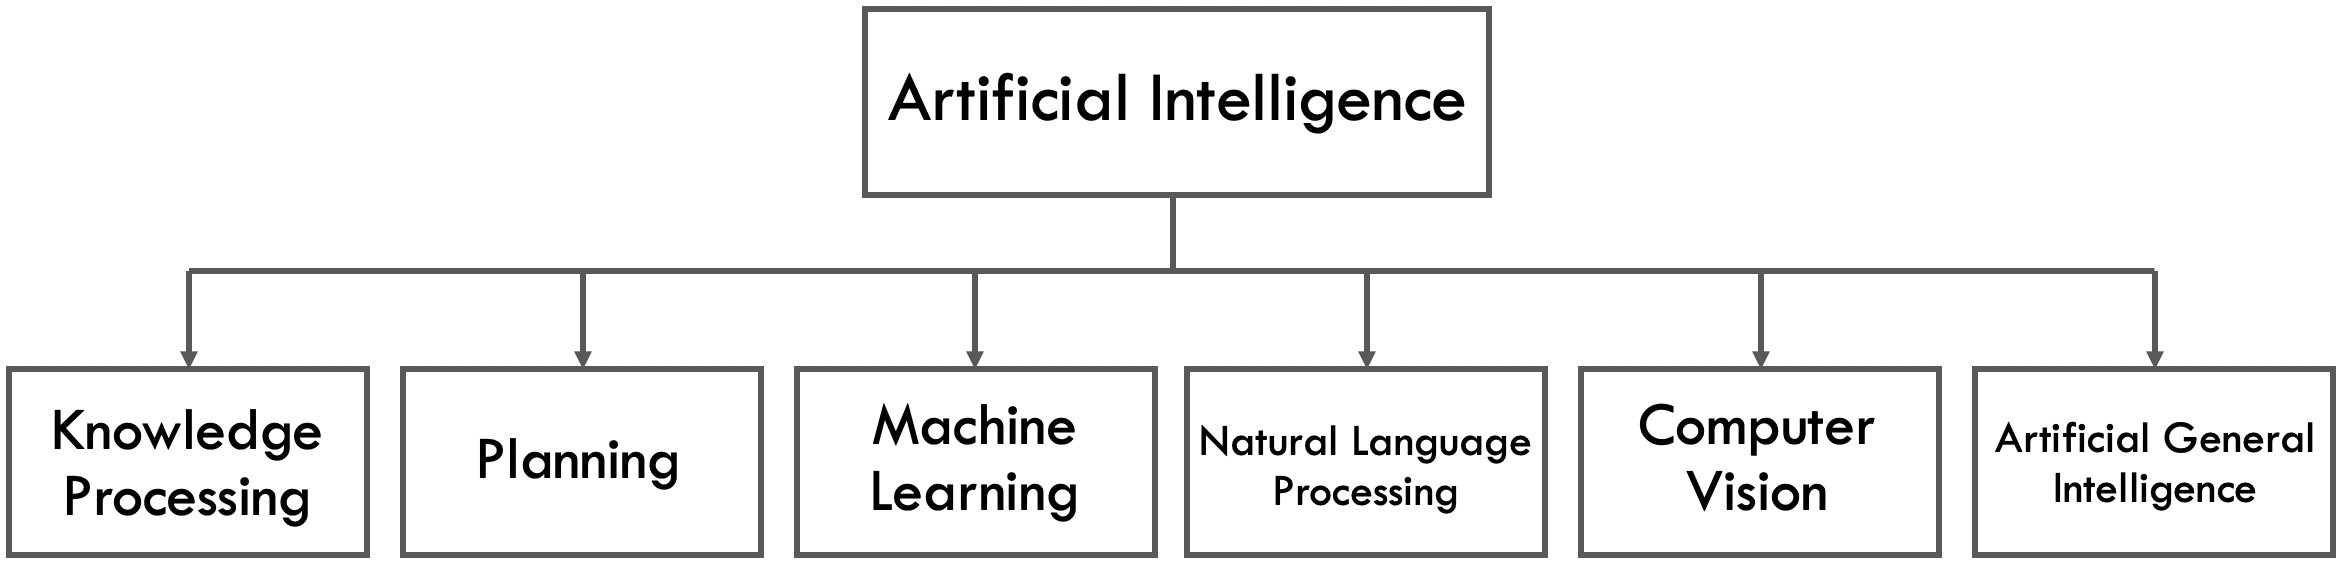
\includegraphics[width=\textwidth]{images/ch1/AIGoals.jpeg}
    \caption{The major goals of artificial intelligence.}
    \label{fig:AIGoals}
\end{figure}   

The sub-fields of ML are shown in Figure \ref{fig:MLGoals}.  In supervised learning, the algorithm learns the optimal input-output mapping, called the model, from a training data set pre-labeled by an external supervisor \cite{sutton}.  Be aware that not all labels provided are guaranteed to be correct. In fact, it is not uncommon to  have mislabeled data caused by noise in the original data set. For example, imagine trying to transcribe an interview with the audio playback heavily corrupted by noise.  In the process industry, the supervisor is typically a sensor measuring the current condition of the process (pressure, temperature, flow rate, etc.) and are often times unreliable. In the end, the performance of the supervised learning model is \textit{upper bounded} by the quality of the labels provided by the supervisor.  In the ideal case, the model can exactly replicate the right \textit{and wrong} labels of the supervisor. In unsupervised learning, the algorithms are typically used to optimally segregate data based on their similarity or to identify the principal components within large data sets \cite{Hinton, sutton}.  Objectively, unsupervised learning identifies hidden patterns within data sets through feature extraction and dimensional reduction. Semi-supervised learning is a hybrid between supervised and unsupervised learning where the models are trained on a small data set of labeled data and refined using features extracted from the unlabeled data set. For example, in the process industry, tasking an engineer to manually label data sets is a costly but required endeavor.  In many applications such as fault detection or root cause analysis, a well labeled data set is required to materialize any useful applications.  Using semi-supervised learning in these scenarios, the model can learn from the small labeled data set and extract additional helpful insights from the remaining unlabeled data to fine tune performance.  In this case, the final algorithm is vastly superior compared to its supervised or unsupervised learning counterpart \cite{machine_learning}.  Unfortunately, all the above methods exhibit one critical flaw: \textit{the inability to transcend the supervisor in terms of performance}. Although these methods may provide great cost reductions and/or greatly speed up production through automating trivial tasks, the methods fail to expand the current capabilities of modern methods.

\begin{figure}[H]
    \centering
    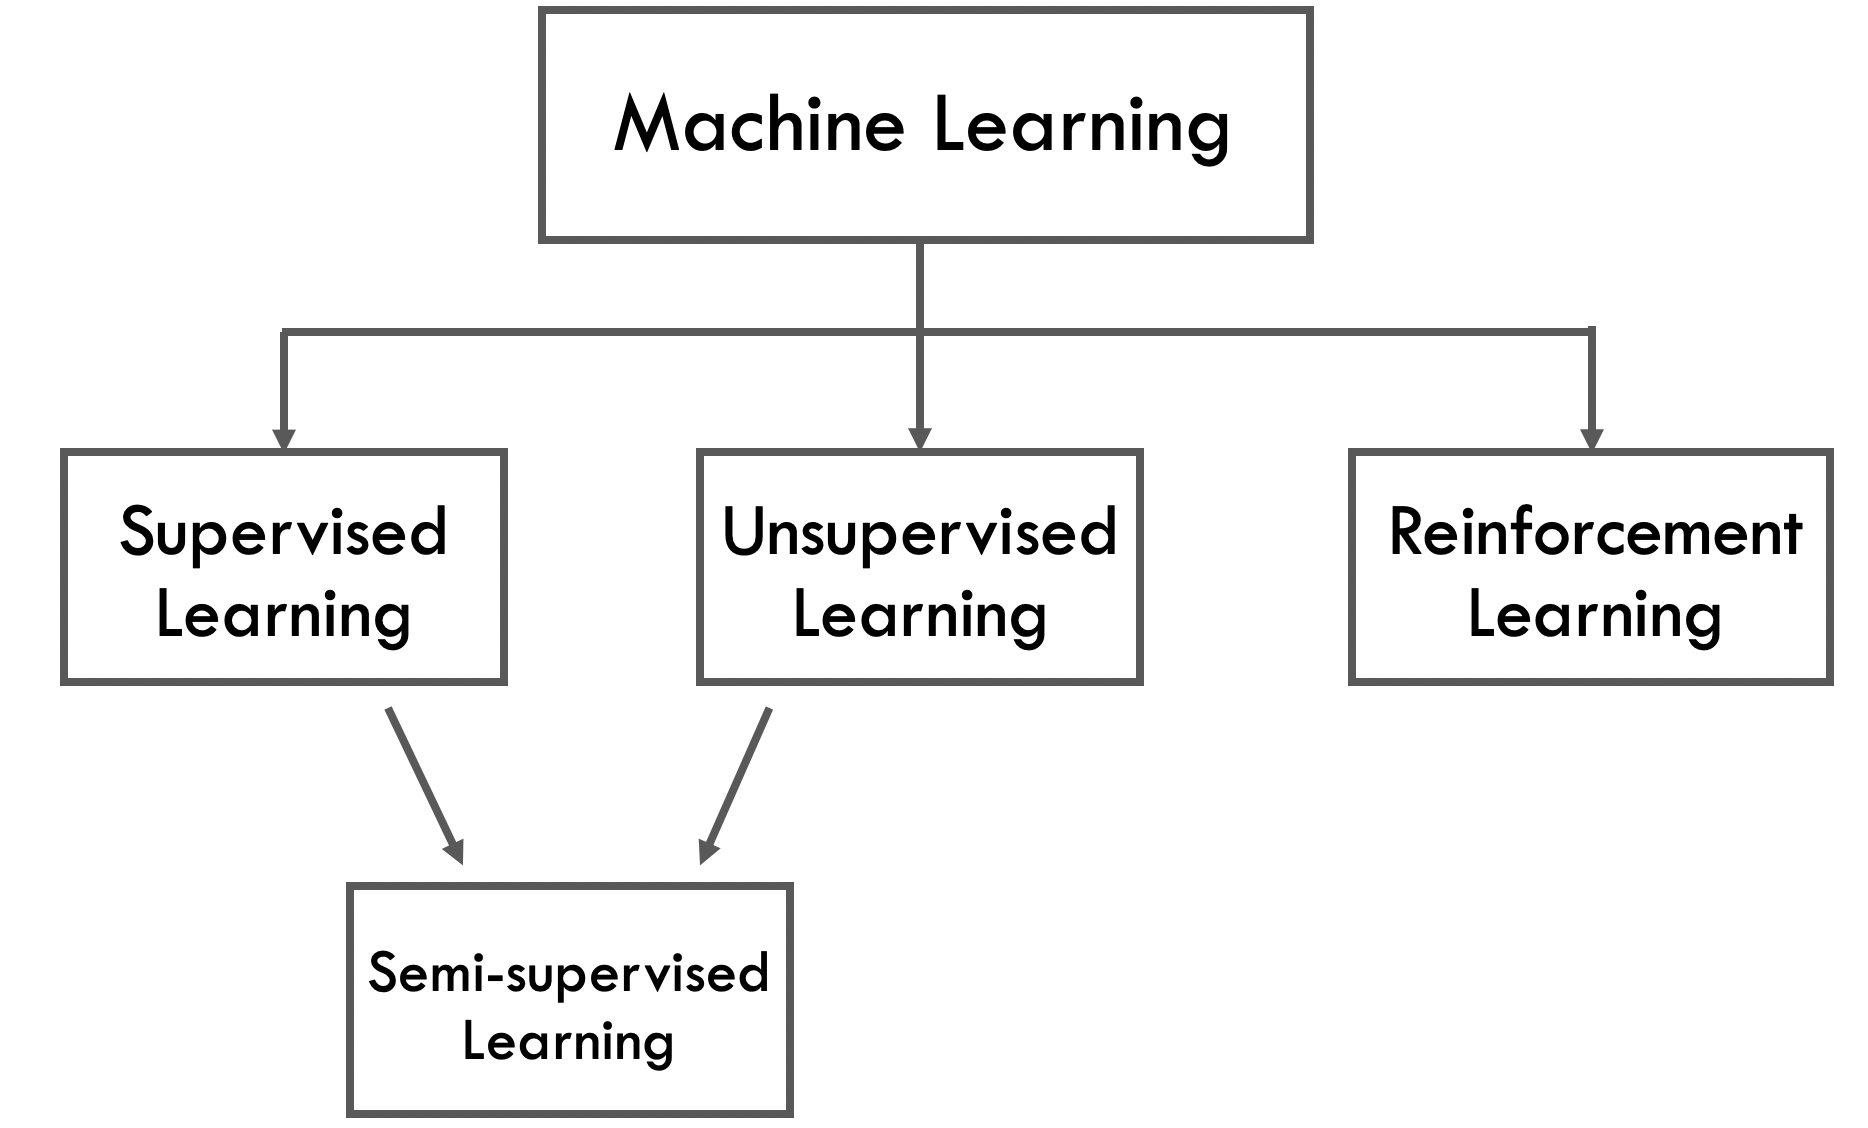
\includegraphics[width=0.6\textwidth]{images/ch1/MLGoals.jpeg}
    \caption{The sub-components of machine learning.}
    \label{fig:MLGoals}
\end{figure}   

Reinforcement learning (RL) aims to overcome this dilemma by providing machines the ability to \textit{surpass all known methods}.  More specifically, reinforcement learning \textit{agents} learns the optimal actions to perform in different situations (also called optimal policy) through self-interaction with the environment.  After each interaction, the agent is provided feedback via a scalar reward signal; large positive rewards follow good actions while negative rewards follow bad actions.  In challenging circumstances, actions affect both the immediate reward signal and the subsequent rewards there-forth. In an intuitively context, pursing an University degree may yield negative immediate rewards; however, rewards years down the line may become significantly more positive due to the newly equipped knowledge.  These two characteristics---delayed feedback and guided trial-and-error search---differentiate RL from all other types of algorithms and ultimately permit RL to push the existing boundaries of known science \cite{sutton}.


\section{Motivation and Challenges}
The non-existent price recovery of the Western Canadian Select crude index since its collapse in 2015 has forced many Canadian energy companies to shift their operating strategies from expansion to optimization \cite{oil_price}.  Typically, existing processes in the oil and gas sector are old and have been operating in a similar regime for many years.  In doing so, vast amounts of data have been collected for the current operating regime.  Through rapid advancements of computer hardware, this data can now be leveraged as a gold mine for modern data hungry machine learning algorithms.  Firstly, the data can be used for predictive applications such as forecasting, digital twinning, soft sensing, and even training purposes.  The data can also be leveraged to create "ML-assisted" safety applications similar to driver assistance in the automotive industry. For example, process monitoring and process forecasting ML models can be built to \textit{proactively} manage operational risk by identifying hazards well in advance of actual incidents. Modern optimal control methods (i.e., maximizing profits of a plant or minimizing operating cost) can also benefit greatly through the assistance of ML algorithms.  Currently, a common optimal control method is MPC; however, the method assumes the availability of an accurate process model.  In any industrial scale process, an accurate process model is nearly impossible to identify due to the vast amount of non-linear interaction effects.  Even after identification, the model would need re-tuning after several months due to process drifts and other changes. Furthermore, for large processes, the dimension of the states and actions may be too large for online optimization to be feasible. One field of study called distributed MPC aims to solve this computational hurdle by decomposing the system into smaller sub-systems; however, distributed MPC performance are typically subpar compared to its centralized counterpart due to communication issues \cite{distributed_mpc}. Through RL, such large problems may be computationally feasible as a centralized algorithm by pre-computing the optimal control policies offline. Moreover, process drifts can be naturally handled by RL through its direct adaptive optimal control nature \cite{direct_adaptive}.  For traditional optimal control, adaptive characteristics are typically indirect and require re-identification of the system models.  In the case of RL, the policy is  adapted directly through interactions with the environment. Although there exists numerous machine learning success stories in the technology sector, their applications in the process industry is still severely limited. One main reason for the absence of recent ML progress is the lack of a workforce skilled in both ML and process control.

Many technology companies and ML engineers specialized in the technology sector have attempted to fill the gap; however, process control data is exceedingly different compared to traditional image or transactional data.  The data in process control is typically unintuitive, time-series, and are often times unreliable or noisy.  There also exists many time delays in chemical processes and feature engineering is difficult without proper fundamentals of process engineering. Comparatively, the data in the technology sector is often very intuitive and easy to understand.  For example, building a classification algorithm for facial recognition is easier to understand compared to predicting when a pump will fail.  The former only requires an image of the individual or some 3D spatial data corresponding to the individual's facial features. In the latter, there may be thousands of interactions affecting the ultimate outcome of the pump, most of which are impossible to identify through intuition alone. Due to these differences, engineers not specialized in the process sector faced great challenges when attempting to create value in the process industry.

More recently, there has been a surge of ML innovations made by research scientists and AI start-up companies catered towards the process industry.  However, most were never commercialized because the mentality between industry and the engineers were vastly different.  In industry, the ultimate objective is to create shareholder value through risk-managed products; it may be traditional methods or it can be ML.  For the research scientists, the focus is more on the elegance and novelty of the algorithm, no matter the complexity. For industry, such algorithms are difficult to explain to a non-technical audience, have a high cost of ownership for the customer, and are difficult to understand without a team of subject matter experts (which themselves cost a significant amount of money).

Throughout this thesis, the main theme is to introduce easy, cost effective solutions that explicitly considers the following four customer focused values required for successful commercial products \cite{marketing}:
\begin{itemize}
    \item \textbf{Functional value:} Describes the overall usefulness of the product compared to other available products.  For example, a ML anomaly detection algorithm may be far superior compared to other methods if enough data is present.
    \item \textbf{Monetary value:} The cost savings generated from this product (e.g., amount of money saved through using an optimization algorithm or preventing a loss incident).  
    \item \textbf{Social value:} Ability for the product to enhance your brand or product awareness and is especially important for sales focused enterprises.  For example, after an individual goes to Disneyland, they may tell many people how great it was without any incentive from Disney.  In the process industry, operators and/or engineers will recommend great products that helped them in their jobs and/or become more productive without external incentives.
    \item \textbf{Psychological value:} Ability to make the company feel superior compared to the competition.  For example, a firm may believe they have better chances at winning contracts if their products contain state-of-the-art ML technology needed for big data applications.
\end{itemize}
Ultimately, the goal is to create organic growth for the local industry through new, innovative ways.  If an exceptionally complex solution is engineered, but there exists no customers, the solution didn't end up solving anything.

\section{Thesis Outline and Contributions}
The thesis is organized as follows: First, basic concepts of RL and MPC will be introduced.  In Chapter 2, applications of ML algorithms in prediction applications will be explored on an industrial pipeline.  Following that, ML for process safety applications will be shown in Chapter 3. Safety applications include topics such as anomaly detection, anomaly prediction, and alarm management. Up until Chapter 3, the projects will use exclusively traditional supervised, unsupervised, and semi-supervised learning methods because the applications are predictive in nature.  Towards the end of Chapter 3 until the end of the thesis, RL methods will be introduced because these applications are more control oriented. Chapter 4 contain various different RL applications in process control. Applications here include the optimal control of a waste water treatment plant, set point tracking control of small scale systems, and fault-tolerant control of an industrial distillation tower. Additionally, RL is also compared to MPC on simple small-scale systems in this chapter. Finally, this thesis is concluded in Chapter 5.  A comprehensive project report for the pipeline optimization project introduced throughout this thesis is shown in Appendix A.

The contributions of this thesis is as follows: In Chapter 2, methods for identifying representative process models in an industrial settings are introduced. Additionally, a new adaptive modelling method was formulated here to significantly reduce the cost of ownership of the machine learning models for the industrial partner. The adaptive method also overcomes catastrophic interference and can be retrofitted onto all model structures. Chapter 3 introduces novel data pre-processing approaches to anomaly detection and prediction in the process industry.  Additionally, a new RL-powered alarm management method is introduced for filtering of nuisance alarms, alarm reduction, and alarm prioritization.  Chapter 4 provide comparisons between traditional optimal control methods with RL on many different systems. Furthermore, a new easy-to-implement continuous non-linear RL method is also shown here.  The last contribution in Chapter 4 is the extension of RL into a fault-tolerant control where RL is used for both the fault detection algorithm and the fault tolerant controller. 


%%%%%%%%%%%%%%%%%%%%%%%%%%%%%%%%%%%%%%%%%%%%%%%%%%%%%%%%%%%%%%%%%%%%%%%%%%%%%%%%%%%%%
% Bandits
%%%%%%%%%%%%%%%%%%%%%%%%%%%%%%%%%%%%%%%%%%%%%%%%%%%%%%%%%%%%%%%%%%%%%%%%%%%%%%%%%%%%%

%%%%%%%%%%%%%%%%%%%%%%%%%%%%%%%%%%%%%%%%%%%%%%%%%%%%%%%%%%%%%%%%%%%%%%%%%%%%%%%%%%%%%
% Bandits
%%%%%%%%%%%%%%%%%%%%%%%%%%%%%%%%%%%%%%%%%%%%%%%%%%%%%%%%%%%%%%%%%%%%%%%%%%%%%%%%%%%%%

\section{Preliminaries to Reinforcement Learning}

Reinforcement learning is a goal-directed learning algorithm which continually improves its own performance through interactions with the environment \cite{sutton}. The main objectives of reinforcement learning are to identify hidden structures within the environment and to find the optimal policy (i.e., optimal state to control action mapping) through guidance from an internal scalar reward (feedback). Two distinct characteristics that deviate reinforcement learning from other methods are its trial \& error search to find the optimal policy, and its ability to identify delayed reward signals. Modern reinforcement learning methods combine principles of optimal control and learning methods together to solve for the optimal control trajectory in an environment.  In the remaining sections of this chapter, fundamental reinforcement learning concepts will be introduced.  Then, tabular based RL methods will be shown.  However, due to the "curse of dimensionality" of high dimensional problems, tabular based approaches struggle in large multi-variate scenarios.  To overcome these issues, deep neural networks will be leveraged for function approximation, and deep reinforcement learning will be introduced.

\subsection{A historical overview}
Reinforcement learning is a combination of two fields of research: \textbf{optimal control} through extremizing an objective function through dynamic programming and \textbf{animal psychology} inspiring trial-and-error search. Originally, the \textbf{optimal control} problem was proposed for designing controller to maximize or minimize the objective function of a dynamical system over time \cite{mpc}.  By the 1950s, Richard Bellman extended on the works of Hamilton and Jacobi to develop a novel approach to solve the optimal control problem.  This approach, known as dynamic programming, optimizes a system's input trajectory by using the functional equation (a function where the unknowns are also functions) generated from the system's state information together with a value function \cite{bellman1}.  The functional equation, now called the Bellman equation, is mathematically represented as:
% Will leave spaces during submission for reviewers
\begin{equation}
    V(x) = r(x) + \gamma \sum P(x' | x, u) \cdot V(x')
    \label{eq:bellman_eq}
\end{equation}
where $V(x)$ represents the value function of $x$. Here, $\gamma$ denotes the discount factor to incorporate future uncertainty. $r(x)$ is the reward signal obtained as a function of the system's desired performance. $P(x'|x, u)$ is the dynamics function describing the transitional probability of arriving at state, $x'$, given $x$ and $u$. $V(x')$ is the value function of $x'$. Intuitively, the value function describes how good or how bad being in particular state is, assuming optimal behaviour thereafter; high values represent good states and low values for bad.  True dynamic programming is "cursed by dimensionality" (i.e., computational cost increases exponentially with the dimensions of the states and actions); thus, approximate dynamic programming (ADP) methods were developed to bypass this hurdle \cite{adp}.  In reinforcement learning, many ADP methods are leveraged to solve for the optimal policy. The concept of a feedback oriented learning system in RL originated from \textbf{animal psychology}. More specifically, the original concept was introduced in the early $20^{th}$ century, named the "Law of Effect". The law stated that animals tend to repeat actions resulting in good outcomes, vice versa for actions with bad outcomes \cite{thorndike}. Initially, the agent explores the environment in which it exists to identify the outcomes corresponding to different actions, then only repeating the actions resulting in good outcomes thereafter. By unifying dynamic programming from optimal control and trial-and-error search from animal psychology, the modern field of RL was developed. For a more comprehensive overview of the history of RL, see \cite{sutton}.

The development of RL is shown in Table \ref{tab:RLevo}.  Reinforcement learning takes its roots from the \textit{k}-armed bandit problem that has been extensively studied in engineering, psychology, and statistics.  This problem disregards state information, and only worries about solving the optimal actions for \textit{one} specific situation \cite{thompson1, thompson2, robbins, bellman_bandit}.  As a natural extension, Barto, Sutton and Brouwer expanded the idea to multi-situation systems \cite{bartosuttonbrouwer} through associative search, also known as \textit{contextual bandits}. The main objective of this algorithm was to find an optimal policy, $\pi^*(x)$, for each situation.  However, it only concerns the immediate rewards and not the long term consequences. Reinforcement learning was then developed to find the optimal policy for different situations based on immediate reward and the onward trajectory there-forth.  

\begin{table}[H]
\caption{From left to right, the evolution of reinforcement learning.}
\centering
\begin{tabular}{c|c|c}
\textbf{$k$-armed bandits}	& \textbf{Contextual bandits}	& \textbf{Reinforcement learning}\\
\hline
Optimal action		  & Optimal action			& Optimal action \\
One situation		  & Many situations			& Many situations \\
Immediate consequence & Immediate consequence	& Long-term consequence \\
\end{tabular}
\label{tab:RLevo}
\end{table}

\subsubsection{\textit{k}-armed Bandit}

The \textit{k}-armed bandit problem provides the fundamentals to understanding modern reinforcement learning.  Here, an agent is present and must choose action $u$ from $\mathcal{U}$, where $\mathcal{U}$ has $k$ choices.  After each action, a scalar reward from a stationary distribution will be returned to the agent as feedback. Favorable actions yield positive rewards, while unfavorable actions return negative rewards. The objective of the agent is to ultimately maximize reward over $N$ steps.  For each action, there is an expected reward called \textit{value}, given by Equation \ref{eq:01value}.

\begin{equation}
    \centering
    q_*(u) = \mathbb{E}[R_t | U_t = u]
    \label{eq:01value}
\end{equation}
where $u$ is the action taken at time, $t$.  $R_t$ is a scalar reward returned to the agent after action $u$ was performed at time $t$. $R_t$ is drawn from a stationary distribution, $R_t \thicksim N(q_*(u), \sigma^2)$. Finally, $q_*(u)$ is the expected reward of taking action, $u$.

The real value is unknown, however, an estimation can be computed and is denoted as $Q_t(u)$.  Given all $Q_t(u)$ is maintained, at any time, one $Q_t(u)$ will be greater than all others. Picking the action that corresponds to the maximum $Q_t(u)$ is known as \textit{greedy}, and the agent is said to be \textit{exploiting}.  If a non-maximum action is picked, the agent is \textit{exploring} \cite{sutton}.

Action selection based on estimating the value of actions are called \textbf{Action-value methods} \cite{action_value_method}. At time $t$, the estimate of the value is given by Equation \ref{eq: value_est} \cite{sutton}.

\begin{equation}
    \centering
    Q_t(u) = \
    = \frac{\sum_{i=1}^{t - 1} R_i \mathbbm{1}_{U_i=u}}
    {\sum_{i = 1}^{t - 1} \mathbbm{1}_{U_i = u}}
    \label{eq: value_est}
\end{equation}
where $\mathbbm{1}$ equals 1 if the condition is true, else 0.  $R_i$ is the reward obtained at the $i^{th}$ episode through selecting action, $U_i$.  Intuitively, the numerator is the sum of rewards when action, $u$, was taken prior to $t$.  Likewise, the denominator is the number of times action, $u$, was taken prior to $t$. As $t \rightarrow \infty$, $Q_t(u) \rightarrow q_*(u)$.  Action selection is based on Equation \ref{eq: bandit_action_selection}.

\begin{equation}
    \centering
    U_t = \argmax_u Q_t(u)
    \label{eq: bandit_action_selection}
\end{equation}

However, initial successful episodes may cause the agent to be stuck at local minimums. To overcome this, a semi-stochastic action selection method called $\epsilon$-greedy can be introduced to promote exploration. In this method, the agent will perform a random action with $\epsilon$ probability (greedy action can be performed).  Higher $\epsilon$ results in more exploratory moves.  Consequently, all $u \in \mathcal{U}$ will be picked many times and by the law of large numbers, $Q_t(a) \rightarrow q_*(a)$ \cite{large_numbers}. Figure \ref{fig: eps_figure} shows the effect of $\epsilon$ on the performance of the agent.

\begin{figure}[H]
    \centering
    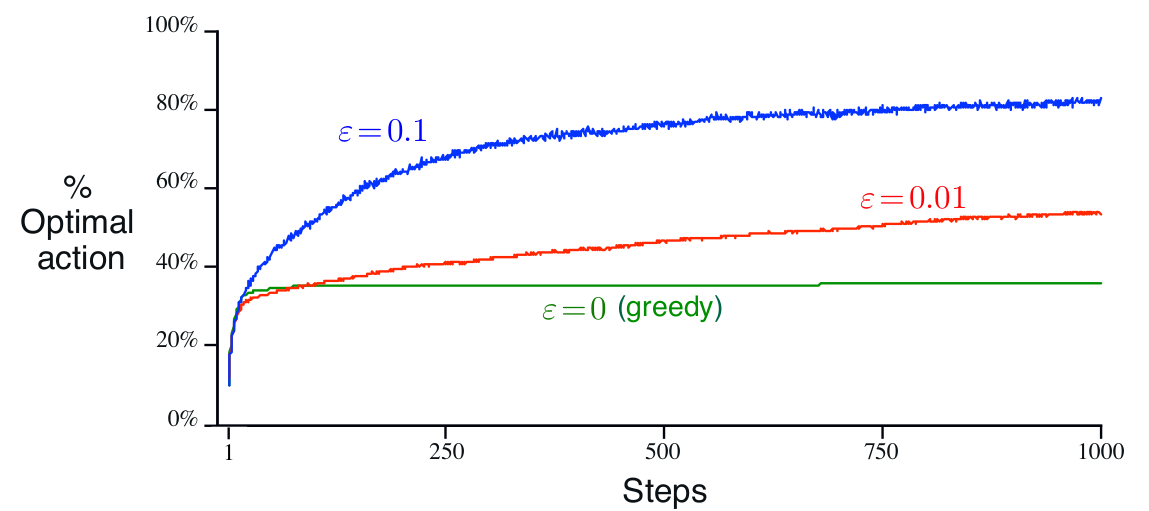
\includegraphics[scale=0.35]{images/eps_vs_optAction.png}
    \caption{Average performance of three agents using different $\epsilon$.  The data is averaged over 2000 runs.  Figure from \textit{Reinforcement Learning: An Introduction} by Sutton and Barto (2018).}
    \label{fig: eps_figure}
\end{figure}

During implementation, $\epsilon$ should decay out as $Q_t(a)$ approaches $q_*(a)$ to ensure knowledge of the agent is being adequately exploited. For non-stationary problems, $\epsilon > 0 \; \forall t$ to ensure other action values have not changed.

Algorithms to solve the \textit{k}-armed bandit problem are easily applied to situations where the concept of state is inert and only the actions are of concern;  a near impossibility in the real world.  

\subsubsection{Contextual Bandit}

A natural extension of the \textit{k}-armed bandit is associative search.  In associative search (sometimes called contextual bandit), different policies are associated with different situations \cite{bartosuttonbrouwer}.  Equation \ref{eq: state-action-value} is the extension of Equation \ref{eq:01value} in the associative search problem.

\begin{equation}
    \centering
    q_*(x, u) = \mathbb{E}[R_t | X_t = x, U_t = u]
    \label{eq: state-action-value}
\end{equation}

Associative search is known as the method between \textit{k}-armed bandits and reinforcement learning.  In associative search, the objective is to associate optimal policies to different situations, but only maximizing the \textit{immediate} reward.  Often times, near term sacrifices are required to initiate the trajectory to a large lump sum reward at the terminal state.  For example, heavy capital and time investment is required for University in the short term.  However, the long term gain is so great that it outweighs the short term losses, making going to University an optimal policy for many individuals.

In order to find the true optimal policy (i.e., policy that returns the greatest rewards over a long time period), the topic of reinforcement learning is developed.  In reinforcement learning, sequential decision making is explored to identify the delayed reward signals from different actions and to ultimately find the optimal policy, $\pi^*$.  

%%%%%%%%%%%%%%%%%%%%%%%%%%%%%%%%%%%%%%%%%%%%%%%%%%%%%%%%%%%%%%%%%%%%%%%%%%%%%%%%%%%%%
% MARKOV DECISION PROCESSES
%%%%%%%%%%%%%%%%%%%%%%%%%%%%%%%%%%%%%%%%%%%%%%%%%%%%%%%%%%%%%%%%%%%%%%%%%%%%%%%%%%%%%

%%%%%%%%%%%%%%%%%%%%%%%%%%%%%%%%%%%%%%%%%%%%%%%%%%%%%%%%%%%%%%%%%%%%%%%%%%%%%%%%%%%%%
% MARKOV DECISION PROCESSES
%
% Introduction to MDPs, finite MDPs, infinite MDPs
% Semi MDPs
% Partially Observable MDPs
%
%%%%%%%%%%%%%%%%%%%%%%%%%%%%%%%%%%%%%%%%%%%%%%%%%%%%%%%%%%%%%%%%%%%%%%%%%%%%%%%%%%%%%

\section{Markov Decision Processes}
In the face of uncertainty, the agent's \textit{sequential} decision making is formalized in the Markov decision process (MDP). The general MDP framework is shown in Figure \ref{fig:01mdp} and contains two components: the \textbf{agent} and the \textbf{system}. The \textbf{agent} is a continuously learning decision maker and is mathematically represented by the RL algorithm. Objectively, the agent will undergo numerous meaningful interactions with the system to ultimately learn the optimal policy, $\pi^*$ (i.e., the optimal decisions given different situations). Conversely, the \textbf{system} contains all elements the agent cannot arbitrarily control. In process control, the ambient temperature, actuators, and even the wires transporting the control signals are all part of the system because the agent cannot \textit{deterministically} manipulate them. 

\begin{figure}[H]
    \centering
    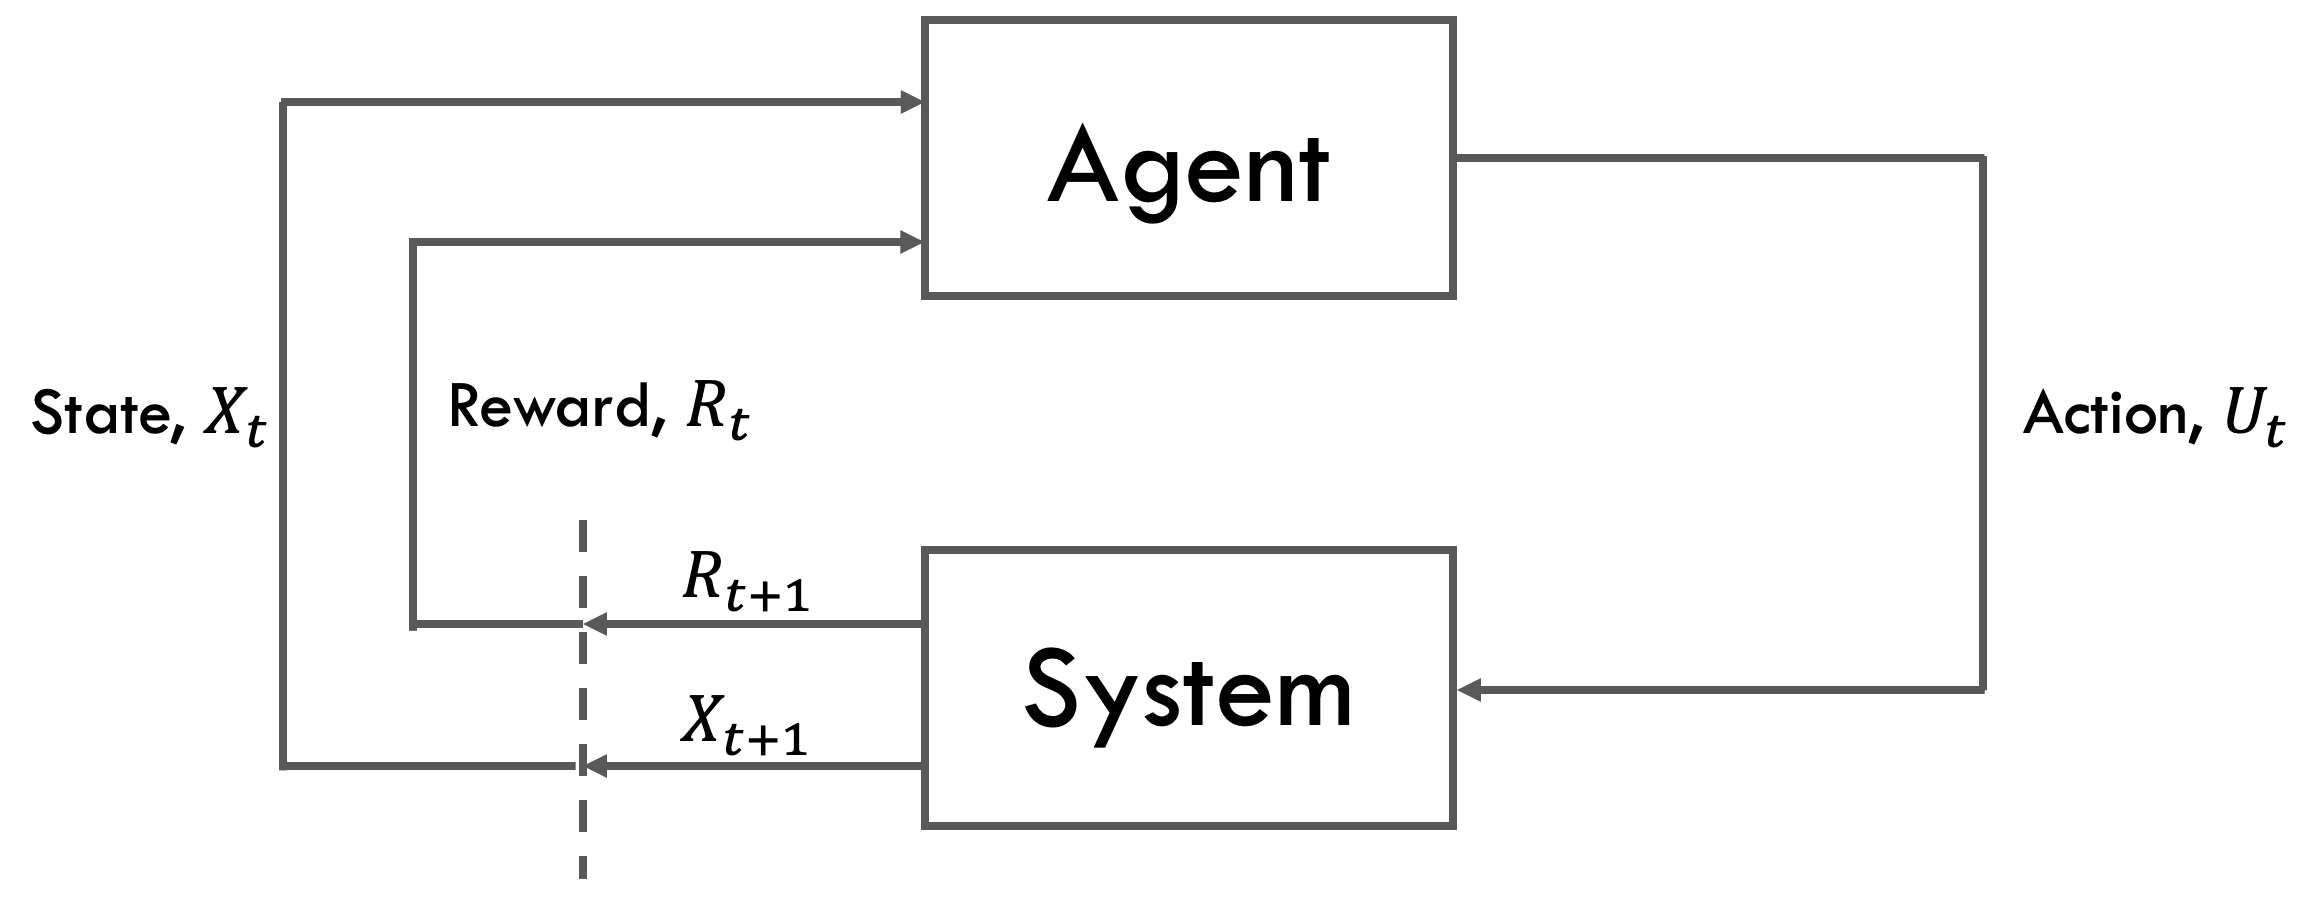
\includegraphics[width=0.56\textwidth]{images/ch1/MDP.jpeg}
    \caption{The general Markov decision process framework. Original image from \cite{sutton}.}
    \label{fig:01mdp}
\end{figure}   

Mathematically, the MDP is a discrete representation of the stochastic optimal problem and a classical formulation of \textit{sequential} decision making where both the immediate and long term consequences are explicitly considered \cite{bellman1, mdp_bellman}. Many definitions of the MDP exist and are equivalent up to small alterations of the process.  One comprehensive definition is that a MDP is a tuple $\mathcal{M}$, is a tuple $(\mathcal{X}, \mathcal{U}$, $P(x', r|x, u), \gamma, R)$ comprised of the following\cite{ng_ref12}:
\begin{itemize}
    \item $x \in \mathcal{X}$: \textbf{State} space of the system at each time step. Common states in industrial processes include temperatures, valve positions, pressures, flow rates, etc.
    \item $u \in \mathcal{U}$: Bounded \textbf{action} space of the agent, ($\mathcal{U}$ $ \geq 2 $). In traditional control, this is the \textbf{bounded input signals} sent to the actuators.
    \item $R \in \mathbb{R}$: Expected \textbf{reward} signal after performing action $u$ in state $x$. Reward functions are designed based on a desired performance metric.  In control theory, the reward function is known as the \textbf{objective function}.  Typically, $|R| \leq \mathcal{R}$ for convergence guarantees.
    \item $p(x', r|x, u)$: Systems \textbf{dynamics function}. Formally, it is the probability of transitioning to $x'$ and receiving $r$,  given states $x \in \mathcal{X}$ and performing action $u \in \mathcal{U}$. Mathematically, it is described by the following:
    \begin{equation}
        p(x', r | x, u) \dot{=} Pr\{X_t = x', R_t = r | X_{t - 1} = x, U_{t-1} = u\}
        \label{eq:transition_prob}
    \end{equation}
    where $p$ describes the system \textbf{dynamics} and $Pr$ denotes the probability operation \cite{sutton}. Additionally, $p$ satisfies the following equality:
    \begin{equation}
        \sum\limits_{x' \in \mathcal{X}} \sum\limits_{r \in \mathcal{R}} p(x', r | x, u) = 1, \forall x \in \mathcal{X}, u \in \mathcal{U}
        \label{eq:prob}
    \end{equation}
    Notice here that $p$ is only a function of the \textit{immediate past}, thus assuming that $x_{t - 1}$ and $u_{t-1}$ captures the complete history. This is known as the Markov property and its underlining assumptions are critical for successful process control applications using RL. Additionally, note that when the state and actions are formulated as augmented past information: $x_{t-1} = [s_{t-1}, s_{t-2}, ... s_{t-N}], u_{t-1} = [a_{t-1}, a_{t-2}, ..., a_{t-N}]$, where $s_{t-N}$ and $a_{t-N}$ denotes the past states and actions, the system is still Markov because decisions can be made exclusively using $x_{t-1}$ and $u_{t-1}$. 
    \item $\gamma$: \textbf{Discount factor} associated with uncertainty of the future, ($0 \leq \gamma \leq 1)$. $\gamma < 1$ is also a requirement for continuous processes to guarantee eventual convergence.
\end{itemize}

There exists three different MDPs: fully observable MDP (FOMDP), partially observable MDP (POMDP), and semi MDP (SMDP). Table \ref{tab:01mdps} shows a general guideline on the different MDPs.

\begin{table}[H]
\caption{A comparison of different Markov decision processes.}
\centering
\begin{tabular}{c|c|c}
\textbf{FO-MDPs}	& \textbf{S-MDPs}	& \textbf{PO-MDPs}\\
\hline
All states observable		  & All states observable			& Some states observable \\
Discrete time		          & Continuous time	             	& Discrete time \\
\end{tabular}
\label{tab:01mdps}
\end{table}

\subsection{Fully observable Markov decision processes}
Fully observable Markov decision processes are the simplest and serves as the foundational framework.  They are mainly applied to discrete systems with fixed sampling times where transition dynamics are unimportant and all states are observable (measurable in control literature). Here, the agent starts in some initial states, $x_0$. At each time $t$, the agent maps $x_t$ to some $u_t$ corresponding to its policy, $\pi_t$.  Given $x_t$ and $u_t$, the system will then transition to some new states $x_{t+1}$ dictated by Equation \ref{eq:transition_prob} while outputting reward signal $R_{t+1}$ based on the reward function. In regulation and set-point tracking problems, this reward function is typically the squared tracking error between $x_t$ and $x_{sp}$.  By repeating this cycle many times, the agent is able to traverse through some sequence, $x_t, u_t, R_{t+1}, x_{t+1}, u_{t+1}, R_{t+2}, x_{t+3}, ...$ and accumulate \cite{sutton}:
\begin{align}
G_t &= R_{t+1} + \gamma R_{t+2} + \gamma^2 R_{t+3} ... \\
    &= \sum\limits^{\infty}_{k = 0} \gamma^k R_{t+k+1}
\label{eq:return}
\end{align}
where $G_t$ denotes the cumulative discounted return at time $t$ and $\gamma$ is the discount factor to capture the future uncertainty. MDPs can represent both finite or infinite systems; the former describes episodic tasks with explicit terminal states while the latter describes tasks that continue forever.  Intuitively, most two-player board games such as Checkers, Chess, or Go are finite MDPs where the game is terminated after one player is defeated.  Contrarily, an infinite MDP system could be the control system in an industrial process. For infinite MDP systems, $\gamma < 1$ is a necessary condition to keep $G_t$ bounded. Ultimately, the agent is tasked with finding the optimal policy, $\pi^*$, that maximize $G_t$, and subsequently the value function, over $N$ steps. The value function for each state is given as \cite{sutton}:
\begin{align}
    v_\pi (x) &\dot{=} \mathbb{E}_\pi [G_t | X_t = x] \\
              &= \mathbb{E}_\pi \left[\sum\limits^\infty_{k=0} \gamma^k R_{t+k+1} | X_t = x \right] \\
              &= \mathbb{E}_\pi [R_{t+1} + \gamma G_{t+1} | X_t = x]
    \label{eq:value_func}
\end{align}
where $v_\pi (x)$ is the value function of $x$ under policy $\pi$. Theoretically, the existence and uniqueness of $v_{\pi}$ is guaranteed for continuous systems where $\gamma < 1$ or in systems with guaranteed termination.  Compared to Equation \ref{eq:01value}, Equation \ref{eq:value_func} takes the expectation of $G_t$; therefore, explicitly optimizing the long term returns rather than only the immediate rewards. The action-value formulation of Equation \ref{eq:value_func} is:
\begin{align}
    q_\pi (x, u) \; &\dot{=} \; \mathbb{E}_\pi [G_t | X_t = x, U_t = u] \\
                 &= \mathbb{E}_\pi \left[\sum\limits^\infty_{k=0} \gamma^k R_{t+k+1} | X_t = x, U_t = u \right], \forall x, u \in \mathcal{X, U}
    \label{eq:a_value_func}
\end{align}
FOMDPs work well for discrete systems where all states are observable.  However, system states in industrial processes are often unobservable (unmeasurable in control) due to limited hardware or engineering limitations. In such systems, the Markov property no longer holds resulting in sub-optimal decision making of the agent.





\subsection{Partially observable Markov decision processes}
Partially observable Markov decision processes (POMDPs) extend upon the concepts of FOMDPs and represent systems with unobservable states. In RL literature, observability is equivalent to measurability in control; thus, the two terms are used interchangeably here-forth. In FOMDPs, the current state $x_t$ at each time $t$ is fully observable. In the more general setting of POMDPs, the entire state vector describing the agent's current situation is no longer available. Instead, the agent only has access to a set of possible observations $\mathcal{O}$. At each time $t$, the agent sees observation $o_t$ which correspond to probability distributions over states.  Using $o_t$, the agent can infer the states it \textit{might} currently be in \cite{ng_ref12}. Relating to a process control setting, existing sensors typically only measure a subset of the current states; however, by using available measurements, one can infer the remaining unmeasurable states using probabilistic approaches.

Generally, finding $\pi^*$ in a POMDP setting is significantly harder compared to FOMDPs.  Even finding a near-optimal policy is at least NP-hard (non-deterministic polynomial time) \cite{pomdp_time}.  Furthermore, even agents with access to all the system's true value functions are unable to behave optimally in a POMDP setting because the current states are unknown \cite{ng_ref12}. 

Belief states is one method for agents to behave optimally in POMDPs. On a high level, belief states transform the POMDP setting into its FOMDP counterpart through a probabilistic approach. Specifically, belief states, $b$, are probability distributions over states deduced using previous observations and actions. The probability distributions represent what the agent thinks its current state is. Using these probabilities, the agent can compute scalar value functions of each state-action pair and use these to act "optimally".  Note here that the agent's behaviour is optimal given the available information, and not optimal with respect to the system. An quantitative example is provided below:
\begin{quote}
    Suppose an agent exists in a two-input two-output (TITO) POMDP setting with two unobservable states ($x_1$ and $x_2$) and two actions ($u_1$ and $u_2$) and suppose the problem is only concerned with the immediate consequences (for longer horizons, the agent must also consider the long term rewards, making the example less intuitive). In this system, there are four value functions, one for each state-action pair. Suppose $u_1$ earns a reward of 2 in $x_1$ and 0 in $x_2$.  Similarily, $u_2$ earns a reward of 0 in $x_1$ and 1 in $x_2$.  Given $b_t = [0.2, 0.8]$ (probabilities of being in $x_1$ and $x_2$, respectively), then $Q(b_t, u_1) = 0.2 \cdot 2 + 0.8 \cdot 0 = 0.4$ and $Q(b_t, u_2) = 0.2 \cdot 0 + 0.8 \cdot 1 = 0.8$, resulting in $u_2$ being the optimal action.
\end{quote}

In control theory, observers, such as soft sensors, are used to estimate unmeasurable states.  Observers are typically $1^{st}$ principles, data driven, or probabilistic models. The concept of belief states is very similar to observer design in control theory. Traditionally, Kalman filter is a widely used observer design. Conversely, recurrent neural networks (RNNs) are widely used for belief state estimation in RL. The performance of RNN was compared with Kalman filter in \cite{RNNvsKF}, drawing similarities of the two methods' objective, theory, and performance.

System representations using FOMDPs and POMDPs work well in discrete tasks where transition times are constant and transition dynamics are disregarded; however, both topics are paramount for continuous optimal control.  







\subsection{Semi Markov decision processes}
Typical MDPs are discrete representations of the optimal control problem and are sub-optimal in continuous tasks. Semi-Markov decision processes (SMDP) are an extension of MDPs to continuing tasks with unknown transition times and system dynamics. In SMDPs, the transition dynamics of the system are explicitly captured using reward function \cite{continuous_rl_ref14}:
\begin{equation}
R(x_t, x_{t+1}, u_t) = \int\limits^\infty_0 \int\limits^t_0 e^{-\beta s} \rho(x_t, \pi (x_t))dsdF_{x_t, x_{t+1}}(t | \pi (x_t))
\label{eq:reward_rate}    
\end{equation}
where $R(x_t, x_{t+1}, u_t)$ is the expected reward to be received when transitioning from $x_t$ to $x_{t+1}$ after action $u_t$. The rewards, $R$, are calculated at each time step in the transition period to explicitly capture transition information. Then, the average reward of the transition is used to update the agent. Here, $\rho(x_t, \pi(x_t))$ represents the average reward during the transition following policy, $\pi$. $F_{x, x_{t+1}}(t, u)$ denotes the probability distribution of the time required to transition from $x_t$ to $x_{t+1}$.  Finally, $\beta > 0$ denotes the \textit{constant} discount factor in SMDPs, where higher $\beta$ results in short-sighted agents. In SMDPs, the discount factor is corrected for transition time during each update step.  The corrected discount factor is given by:
\begin{equation}
    \gamma(x_t, x_{t+1}, u) = \int\limits^{\infty}_0 e^{-\beta t} dF_{x_t, x_{t+1}}(t | \pi_t)
\end{equation}
where $\gamma (x_t, x_{t+1}, u_t)$ is the expected discount factor that will be applied to the value of state $x_{t+1}$ during the update step shown in Equation \ref{eq:bellman_eq}. The value function for SMDPs is obtained from combining Equations \ref{eq:reward_rate} and \ref{eq:value_func}:
\begin{equation}
v_{\pi}(x_t) = \frac{1 - e^{-\beta \tau}}{\beta} R(x_t, x_{t+1}, \pi(x_t)) + e^{-\beta \tau}v_{\pi}(x_{t+1})
\end{equation}
where $\tau$ is the unknown transition time.  Similarily, the action-value form is given by:
\begin{equation}
    q_{\pi}(x_t, u_t) = \frac{1 - e^{-\beta \tau}}{\beta} R(x_t, x_{t+1}, \pi(x_t)) + e^{-\beta \tau}  q_{\pi}(x_{t+1}, u_{t+1})
\end{equation}
By representing control problems as SMDPs, control strategies resulting in large overshoot, inverse response, or any other undesirable dynamics behaviour can be minimized. Additionally, the system will be able to handle systems with unknown transition times.  An intuitive example illustrating the advantages of SMDPs in process control is as follows:

\begin{quote}
    Suppose a refinery company is operating a continuously stirred tank reactor (CSTR). Objectively, the CSTR must maintain 200$^{\circ}$ C for optimal performance.  The temperature is controlled through a heat exchanger using cold water.  A RL agent was built to optimally control the flow of cold water to maintain the temperature set point. Suppose the CSTR starts at 220$^{\circ}$ C.  Agents using MDP representations may be overly aggressive and send large input signals because the reward is only calculated \textit{right before} the next evaluation step. Therefore, input signals resulting in large overshoot or inverse response may not be reflected in the reward. Contrarily, SMDP representation uses the average reward accumulated along the trajectory to provide feedback to the agent, allowing the transition dynamics to be explicitly captured. This way, input signals resulting in undesirable behaviour can be captured and mitigated. Furthermore, SMDP representations can have flexible evaluation times (traditional representations evaluate after a set time period), enabling re-evaluation during the transitional period and adjusts the discount factor in accordance to the elapsed time from last evaluation.
\end{quote}









\subsection{Optimal solution of the Markov decision processes}
The optimal solution to the RL problem refers to identifying a policy that generates the highest long term returns. Such a policy may not be unique; there may exist many optimal policies, where $v_{\pi^*_1} = v_{\pi^*_2} = ... = v_{\pi^*_N}$.  Formally, the optimal policy must satisfy the \textbf{principle of optimality}: the optimal policy $\pi^*$ is optimal if and only if $v_{\pi^*}(x) \geq v_{\pi \neq \pi^*}(x)$ for all $x \in \mathcal{X}$ \cite{PO}. Mathematically, the optimal value function is:
\begin{equation}
    v^*(x) \dot{=} \argmax_{\pi} v_{\pi}(x), \forall x \in \mathcal{X}
\end{equation}
with its action-value variant being:
\begin{equation}
    q^*(x, u) \dot{=} \argmax_{\pi} q_{\pi}(x, u), \forall x, u \in \mathcal{X, U}
\end{equation}
In a more explicit form, the optimal value function and action-value function written in terms of Equations \ref{eq:value_func} and \ref{eq:a_value_func} are given, respectively, by \cite{sutton}:
\begin{equation}
    v^*(x) = \argmax_{u} \mathbb{E}[R_{t+1} + \gamma v^*(X_{t+1}) | X_t = x, U_t = u]
    \label{eq:01valuefunc}
\end{equation}
\begin{equation}
    q^*(x, u) = \mathbb{E}\left[R_{t+1} + \gamma \argmax_{u_{t+1}} q^*(X_{t+1}, u_{t+1}) | X_t = x, U_t = u \right]
\end{equation}
Here, the $max$ operation denotes that the optimal action will be taken for the remaining of the trajectory. Theoretically, all optimal value functions can be explicitly solved using Equation \ref{eq:01valuefunc}; however, such a task would require unreasonable amounts of computation power for even simple systems. In the following section, three popular methods will be introduced to estimate the value and action-value functions in reinforcement learning.


%%%%%%%%%%%%%%%%%%%%%%%%%%%%%%%%%%%%%%%%%%%%%%%%%%%%%%%%%%%%%%%%%%%%%%%%%%%%%%%%%%%%%
% Reinforcement Learning
%%%%%%%%%%%%%%%%%%%%%%%%%%%%%%%%%%%%%%%%%%%%%%%%%%%%%%%%%%%%%%%%%%%%%%%%%%%%%%%%%%%

%%%%%%%%%%%%%%%%%%%%%%%%%%%%%%%%%%%%%%%%%%%%%%%%%%%%%%%%%%%%%%%%%%%%%%%%%%%%%%%%%%%%%
% Reinforcement Learning
%
% Introduction to MDPs, finite MDPs, infinite MDPs
% Semi MDPs
% Partially Observable MDPs
%
%%%%%%%%%%%%%%%%%%%%%%%%%%%%%%%%%%%%%%%%%%%%%%%%%%%%%%%%%%%%%%%%%%%%%%%%%%%%%%%%%%%

\section{Introduction to Reinforcement Learning}

Reinforcement learning is a goal-directed learning algorithm which continually improves its own performance through interactions with the environment \cite{sutton}. The main objectives of reinforcement learning are to identify hidden structures within the environment and to find the optimal policy (i.e., optimal input trajectory) through guidance from an internal scalar reward (feedback). Two distinct characteristics that deviate reinforcement learning from other methods are its trial \& error search to find the optimal policy, and its ability to identify delayed reward signals. Modern reinforcement learning methods combine principles of optimal control and learning methods together to solve for the optimal control trajectory in an environment.  In this chapter, fundamental reinforcement learning concepts are first introduced.  Then, tabular based methods will be shown.  However, due to the "curse of dimensionality" of high dimensional problems, tabular based approaches fail to bear fruit.  To overcome these issues, deep neural networks will be used for function approximation, and deep reinforcement learning will be introduced.

Reinforcement learning takes its roots from the \textit{k}-armed bandit problem that has been extensively studied in engineering, psychology, and statistics.  This problem disregards state information, and only worries about solving the optimal actions for \textit{one} specific situation \cite{thompson1, thompson2, robbins, bellman_bandit}.  As a natural extension, Barto, Sutton and Brouwer expanded the idea to multi-situation systems \cite{bartosuttonbrouwer} through associative search, also known as \textit{contextual bandits}. The main objective of this algorithm was to find an optimal policy, $\pi^*(x)$, for each situation.  However, it only concerns the immediate rewards and not the long term consequences. Reinforcement learning was then developed to find the optimal policy for different situations based on immediate reward and the onward trajectory there-forth.  

\subsubsection{\textit{k}-armed Bandit}

The \textit{k}-armed bandit problem provides the fundamentals to understanding modern reinforcement learning.  Here, an agent is present and must choose action $u$ from $\mathcal{U}$, where $\mathcal{U}$ has $k$ choices.  After each action, a scalar reward from a stationary distribution will be returned to the agent as feedback. Favorable actions yield positive rewards, while unfavorable actions return negative rewards. The objective of the agent is to ultimately maximize reward over $N$ steps.  For each action, there is an expected reward called \textit{value}, given by Equation \ref{eq: value}.

\begin{equation}
    \centering
    q_*(u) = \mathbb{E}[R_t | U_t = u]
    \label{eq: value}
\end{equation}
where $u$ is the action taken at time, $t$.  $R_t$ is a scalar reward returned to the agent after action $u$ was performed at time $t$. $R_t$ is drawn from a stationary distribution (typically Gaussian), $R_t \thicksim N(q_*(u), \sigma^2)$. Finally, $q_*(u)$ is the expected reward of taking action, $u$.

The real value is unknown, however, an estimation can be computed and is denoted as $Q_t(u)$.  Given all $Q_t(u)$ is maintained, at any time, one $Q_t(u)$ will be greater than all others. Picking the action that corresponds to the maximum $Q_t(u)$ is known as \textit{greedy}, and the agent is said to be \textit{exploiting}.  If a non-maximum action is picked, the agent is \textit{exploring} \cite{sutton}.

Action selection based on estimating the value of actions are called \textbf{Action-value methods} \cite{action_value_method}. At time $t$, the estimate of the value is given by Equation \ref{eq: value_est} \cite{sutton}.

\begin{equation}
    \centering
    Q_t(u) = \
    = \frac{\sum_{i=1}^{t - 1} R_i \mathbbm{1}_{U_i=u}}
    {\sum_{i = 1}^{t - 1} \mathbbm{1}_{U_i = u}}
    \label{eq: value_est}
\end{equation}
where $\mathbbm{1}$ equals 1 if the condition is true, else 0.  $R_i$ is the reward obtained at the $i^{th}$ episode through selecting action, $U_i$.  Intuitively, the numerator is the sum of rewards when action, $u$, was taken prior to $t$.  Likewise, the denominator is the number of times action, $u$, was taken prior to $t$. As $t \rightarrow \infty$, $Q_t(u) \rightarrow q_*(u)$.  Action selection is based on Equation \ref{eq: bandit_action_selection}.

\begin{equation}
    \centering
    A_t = \argmax_a Q_t(u)
    \label{eq: bandit_action_selection}
\end{equation}

However, initial successful episodes may cause the agent to be stuck at local minimums. To overcome this, a semi-stochastic action selection method called $\epsilon$-greedy can be introduced to promote exploration. In this method, the agent will perform a random action with $\epsilon$ probability (greedy action can be performed).  Higher $\epsilon$ results in more exploratory moves.  Consequently, all $u \in \mathcal{U}$ will be picked many times and by the law of large numbers, $Q_t(a) \rightarrow q_*(a)$ \cite{large_numbers}. Figure \ref{fig: eps_figure} shows the effect of $\epsilon$ on the performance of the agent.

\begin{figure}[h]
    \centering
    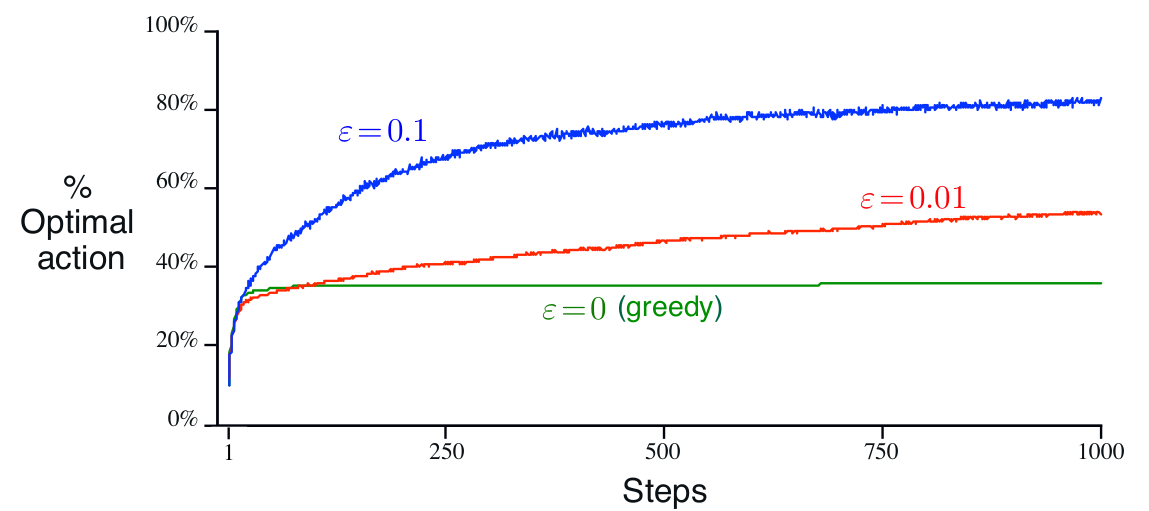
\includegraphics[scale=0.35]{images/eps_vs_optAction.png}
    \caption{Average performance of three agents using different $\epsilon$.  The data is averaged over 2000 runs.  Figure from \textit{Reinforcement Learning: An Introduction} by Sutton and Barto (2018).}
    \label{fig: eps_figure}
\end{figure}

During implementation, $\epsilon$ should decay out as $Q_t(a)$ approaches $q_*(a)$ to ensure knowledge of the agent is being adequately exploited. For non-stationary problems, $\epsilon > 0 \; \forall t$ to ensure other action values have not changed.

Algorithms to solve the \textit{k}-armed bandit problem are easily applied to situations where the concept of state is inert and only the actions are of concern;  a near impossibility in the real world.  

\subsubsection{Contextual Bandit}

A natural extension of the \textit{k}-armed bandit is associative search.  In associative search (sometimes called contextual bandit), different policies are associated with different situations \cite{bartosuttonbrouwer}.  Equation \ref{eq: state-action-value} is the extension of Equation \ref{eq: value} in the associative search problem.

\begin{equation}
    \centering
    q_*(x, u) = \mathbb{E}[R_t | X_t = x, U_t = u]
    \label{eq: state-action-value}
\end{equation}

Associative search is known as the method between \textit{k}-armed bandits and reinforcement learning.  In associative search, the objective is to associate optimal policies to different situations, but only maximizing the \textit{immediate} reward.  Often times, near term sacrifices are required to initiate the trajectory to a large lump sum reward at the terminal state.  For example, heavy capital and time investment is required for University in the short term.  However, the long term gain is so great that it outweighs the short term losses, making going to University an optimal policy for many individuals.

\subsubsection{The Reinforcement Learning Problem}

In order to find the true optimal policy (i.e., policy that returns the greatest rewards over a long time period), the topic of reinforcement learning is developed.  In reinforcement learning, sequential decision making is explored to identify the delayed reward signals from different actions and to ultimately find the optimal policy, $\pi^*$.  

In general terms, reinforcement learning is simply the learning an agent experiences through interactions with the environment.  For added intuition, Figure \ref{fig: simple_rl} shows the generic information flow of reinforcement learning. First, the agent observes some states, $x_t \in \mathcal{X}$, from the environment (some states may be unobservable).  Given $x_t$, the agent performs some actions, $u_t \in \mathcal{U}$ and receives a scalar reward signal, $r_{t+1} \in \mathcal{R}$.  Finally, the environment will transition to a new state, $x_{t+1}$, given probability $P(x_{t+1}, r_{t+1} | x, u)$.

\begin{figure}[h]
    \centering
    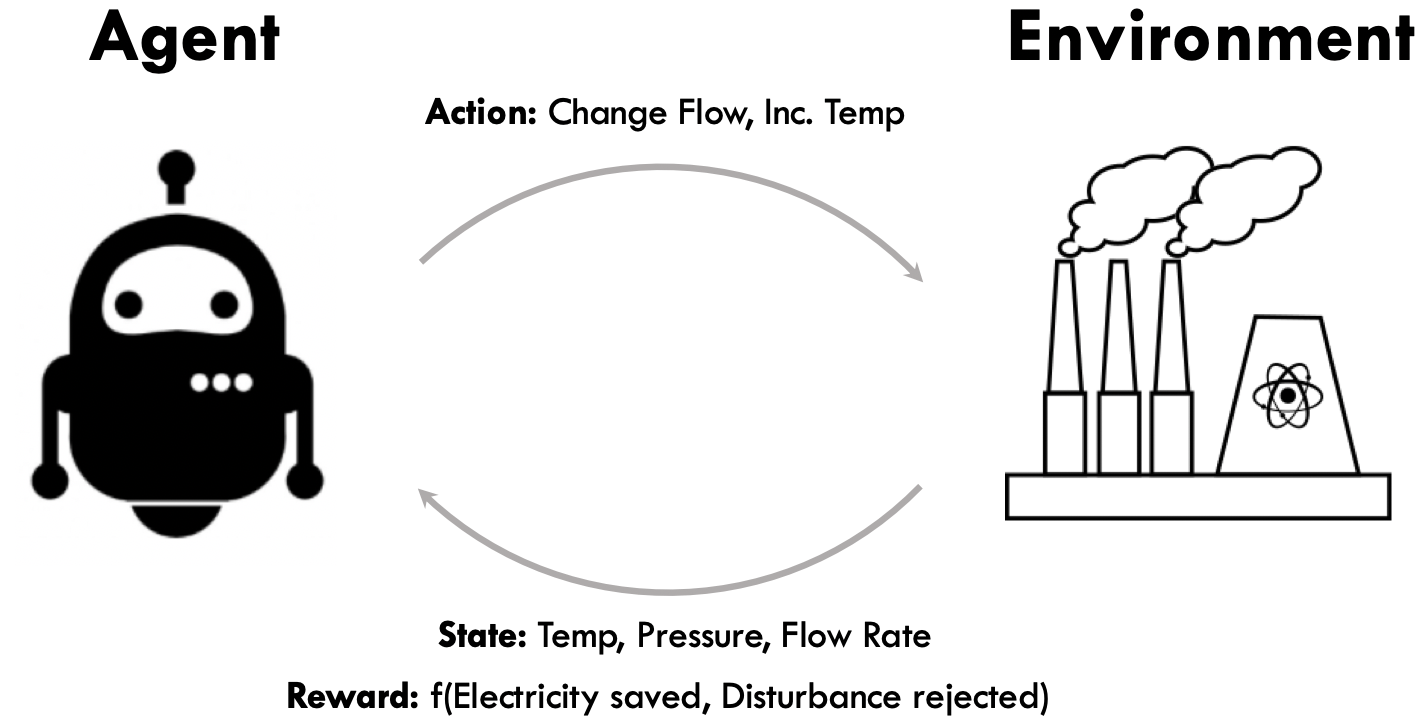
\includegraphics[scale=0.5]{images/RL.png}
    \caption{Basic setup of reinforcement learning where an agent interacts with the environment}
    \label{fig: simple_rl}

\end{figure}

Reinforcement learning consists of the following four elements:

\begin{itemize}
    \item Policy, $\pi$
    \item Reward, $R$
    \item Value Function, $V(s)$
    \item Model (optional), $\dot{x} = Ax + Bu$
\end{itemize}

The policy, $\pi$, of reinforcement learning is a direct mapping from $X \rightarrow U$.  To find the optimal policy, $\pi^*$, the agent is guided by an immediate scalar reward for each interaction (also called \textit{episode}). Policies resulting in higher rewards are more likely to be followed in the future, \textit{mutatis mutandis}.  However, reinforcement learning is concerned with the long term success rather than immediate pleasure. Often times, long term success require short term sacrifice.  Thus, the value function, $V^{\pi}(s)$, is used to describe the long term expected reward under each policy.  Initially, the value function for each state is initialized at zero.  After each episode, the value function will be updated to reflect the new knowledge obtained from the last episode through Equation \ref{eq: value_function}.

\begin{equation}
    \centering
    V(x_t) \leftarrow V(x_t) + \alpha [V(x_{t + 1}) - V(x_t)]
    \label{eq: value_function}
\end{equation}

In Equation \ref{eq: value_function}, $\alpha$ represents the step-size parameter.  That is, how big each update step should be.  Once convergence is achieved for $V(x_t)$, the optimal policy can be described by Equation \ref{eq: opt_policy}.  

\begin{equation}
    \centering
    \pi^*(x) = \argmax_u q_{\pi}(x, u), \; \forall x 
    \label{eq: opt_policy}
\end{equation}

Lastly, reinforcement learning \textit{can} consist of a model. Such cases are called \textit{model-based} reinforcement learning.  The model will be used for planning, and is a way for the agent to plan a control trajectory before they are experienced.  Contrarily, \textit{model-free} reinforcement learning learns \textit{explicitly} through interactions with the environment.

One key topic of reinforcement learning is: \textbf{exploration} vs. \textbf{exploitation}.  At first, the agent must explore to learn the state space, $\mathcal{X}$.  But the agent must know \textit{when} to stop exploring, and start exploiting (i.e., start taking advantage of what is known).  If the agent explores too much, lots of value is lost.  However, if the agent does not explore enough, the current policy may not be optimal and more value is lost long term.  Exploration vs. exploitation is one of the most important topics today in reinforcement learning, and the time to switch from exploration to exploitation will vary between problems.  In control theory, exploration vs. exploitation is known as the conflict between identification (or estimation) and control \cite{explorevexploitcontrol}.  

Another important distinction between different reinforcement learning algorithms is \textbf{on-policy} vs. \textbf{off-policy}.  On-policy methods select actions that maximizes reward given the current knowledge of the agent.  Subsequently, off-policy methods perform exploratory actions for a chance that the explored action offers superior returns to the current best known action.

In the next sub-sections, the three fundamental reinforcement learning methods (Dynamic Programming, Monte Carlo, Temporal-Difference) will be introduced.

\subsection{Dynamic Programming Methods}
\subsubsection{Value-Iteration}
\subsubsection{Policy-Iteration}
\subsection{Monte Carlo Methods}
\subsection{Temporal-Difference Methods}
\subsection{Reinforcement Learning vs. Other "Learnings"}

Machine learning consists of the following four classes: i) Supervised learning, ii) Unsupervised learning, iii) Semi-supervised learning, iv) Reinforcement learning.  Supervised learning is fitting a model to map input data to output data.  The model is initially trained on a set of labeled training data provided by a subject matter expert.  Subsequently, unsupervised learning is used on unlabeled data sets.  The objective of unsupervised learning is to explore the data and identify hidden features. Semi-supervised learning combines the strengths of supervised and unsupervised learning, and is especially useful \cite{machine_learning}.  Often times, industrial data will be partially labelled due to the time and cost associated with data labelling.  For supervised and unsupervised learning, only the labeled and unlabeled data can be used, respectively.  However, all data can be used in semi-supervised learning which allows for maximized data efficiency and increased model performance. Finally, reinforcement learning is a goal-directed learning from interactions with the environment \cite{sutton}.

Reinforcement learning is a unique class of machine learning.  An ideal supervised learning model can only be as good as the subject matter expert providing the labels to the data set, which may not be 100\%.  For example, in a complex control task, the control law is usually highly non-linear. Control experts can try to provide control strategies for such systems, but optimality may not be guaranteed for highly non-linear systems. Also, supervised learning is used to generalize responses for occurrences not present in the data \cite{sutton}.  Reinforcement learning works by directly interacting with the environment \textit{without labels}. Through adequate exploration, reinforcement learning will identify peculiar features to optimally control such problems [citation required].  Reinforcement learning is \textit{similar} to unsupervised learning in terms of identifying hidden structures within the environment.  However, reinforcement learning tries to maximize an internal scalar "reward" signal, rather than purely data mining.

Evolutionary methods, a family of optimization algorithms such as genetic algorithm, are most similar to reinforcement learning.  For a control problem, such methods can apply multiple static policies for different operating regimes \cite{sutton}.  Policy search is conducted by first initiating $k$ random input trajectories of length $N$, generating input matrix $\mathbb{U}_{[k, N]} \in \pi$.  Subsequently, the loss, $J_U$, of each $U$ is calculated based on the objective function.  Input trajectories with the lowest loss move onto the next generation and generates new pseudo-random input trajectories.  This process is repeated until optimal policy, $\pi^*$ is found for each operating regime \cite{ga_for_control}.

Evolutionary methods work well when the policy space is sufficiently small, easy to find, or a lot of time is available for optimization.  The biggest advantage of such methods compared to reinforcement learning is that the whole state does not need to be known.  However, such methods does not capture the reinforcement learning fundamentals of mapping $X \rightarrow U$.  Unlike evolutionary methods, reinforcement learning keeps memory of each indvidual interaction making it a more data efficient approach \cite{sutton}.

%%%%%%%%%%%%%%%%%%%%%%%%%%%%% End Section Intro to RL %%%%%%%%%%%%%%%%%%%%%%%%%%%%%%%%%%%%%%%


%%%%%%%%%%%%%%%%%%%%%%%%%%%%% Begin Section Tabular RL %%%%%%%%%%%%%%%%%%%%%%%%%%%%%%%%%%%%%%

\section{Tabular Q-learning}
\subsection{Introduction to Q-learning}
\subsubsection{Adaptation to Non-Stationary Problems}
\subsubsection{Incremental Implementation}
\subsubsection{Action Selection}
\subsubsection{Exploration in Tabular Q-learning}
\subsubsection{Reward Functions}
\subsubsection{Expected Returns for Different MDPs}

\subsection{Overall Setup}

%%%%%%%%%%%%%%%%%%%%%%%%%%%%% End Section Tabular RL %%%%%%%%%%%%%%%%%%%%%%%%%%%%%%%%%%%%%%%

%%%%%%%%%%%%%%%%%%%%%%% Begin Section Function Approximation %%%%%%%%%%%%%%%%%%%%%%%%%%%%%%%

\section{Function Approximation}
\subsection{Introduction to Function Approximations}
- capture the data of large data set and condense it down into something smaller.
\subsection{Neural Network Basics}
\subsubsection{Neural Network Initialization}
\subsubsection{Gradient Descent Updating}
\subsubsection{Mini-batch Gradient Descent}
\subsubsection{Batch Normalization}
\subsubsection{Regularizations}

%%%%%%%%%%%%%%%%%%%%%%%%% End Section Function Approximation %%%%%%%%%%%%%%%%%%%%%%%%%%%%%%%


%%%%%%%%%%%%%%%%%%%%%%%%%%%%%%%%% Begin Section DDPG %%%%%%%%%%%%%%%%%%%%%%%%%%%%%%%%%%%%%%%

\section{Deep Deterministic Policy Gradient}
\subsection{Actor-Critic Intuition}
\subsection{Actor - Deterministic Policy Gradient}
\subsection{Critic - Deep Q-learning}

\newpage

\subsection{Exploration in DDPG}
\subsubsection{White Exploratory Noise}
\subsubsection{Ornstein-Uhlenbeck Exploratory Noise}
\subsection{Stabilization of Training}
\subsubsection{Experience Replay}
\subsubsection{Target Network}
\subsubsection{Adaptive Batch Gradient Descent}
\subsubsection{Reward Clipping}
\subsection{Input and State Constraints}
\subsection{Training Algorithm}

%%%%%%%%%%%%%%%%%%%%%%%%%%%%%%%%%% End Section DDPG %%%%%%%%%%%%%%%%%%%%%%%%%%%%%%%%%%%%%%%%



\section{Previous RL applications in process control}

%%%%%%%%%%%%%%%%%%%%%%%%%%%%%%%%%%%%%%%%%%%%%%%%%%%%%%%%%%%%%%%%%%%%%%%%%%%%%%%%%%%%%
% Model Predictive Control
%%%%%%%%%%%%%%%%%%%%%%%%%%%%%%%%%%%%%%%%%%%%%%%%%%%%%%%%%%%%%%%%%%%%%%%%%%%%%%%%%%%

%%%%%%%%%%%%%%%%%%%%%%%%%%%%%%%%%%%%%%%%%%%%%%%%%%%%%%%%%%%%%%%%%%%%%%%%%%%%%%%%%%%%%
% Model Predictive Control
%
%
%
%
%%%%%%%%%%%%%%%%%%%%%%%%%%%%%%%%%%%%%%%%%%%%%%%%%%%%%%%%%%%%%%%%%%%%%%%%%%%%%%%%%%%

\section{Model Predictive Control}

Compared to all topics in process control, the concepts of model predictive control (MPC) is perhaps the closest resemblance to modern RL.  MPC is a model-based control strategy (known as a planning method in RL literature) that optimizes the input trajectory of a system by using the functional equation (a function where the unknowns are also functions) generated from the system's state information together with a value function. The performance of MPCs heavily rely on the accuracy of system identification as the input trajectory is solved by extremizing an objective function using mathematical programming (MP) as a function of the process model \cite{mpc}. The objective function is typically given as:
\begin{equation}
    J = \sum\limits^{N}_{i = 1} x_i^TQx_i + \sum\limits^N_{i=1}u_i^TRu_i
    \label{eq:mpc_cost}
\end{equation}
where $N$, $Q$, and $R$ are the prediction horizon and tuning matrices, respectively. Superscript $T$ denotes the transpose operation. $Q$ and $R$ are diagonal matrices and are used to emphasize importance on different state and inputs, respectively. Here, $x$ and $u$ are given as:
\begin{equation}
    x_{sp} - x_i
\end{equation}
\begin{equation}
    u_{ss} - u_i
\end{equation}
where subscripts $sp$ and $ss$ denote the set-point and steady state, respectively. Often times in optimal control, $u_{ss}$ is unknown. In such scenarios, $u$ is given as $\Delta u$ instead, representing a cost in changing the inputs at each step.

Implementation-wise, MPC uses a receding horizon approach where the controller predicts and optimizes for a set amount of steps into the future.  However, only the first control action is implemented.  During the next sampling time, the trajectory is re-optimized and the cycle repeats. The length of the input trajectory and the number of steps the controller predicts into the future are known as the control and prediction horizon, respectively. During design, it is paramount to ensure that both the prediction and control horizons are adequate in length to ensure global optimal solutions.  Intuitively, the prediction and control horizon can be related to the everyday task of driving a car.  It would be very dangerous if we only consider events one second into the future because it would be difficult to react to curves and other road side disturbances; therefore, the prediction and control horizons must be sufficiently long to ensure safe and optimal driving practices. Typically, the control horizon is chosen to be shorter than the prediction horizon due to computational cost and the unimportance of unnecessarily long input trajectories \cite{prediction_horizon}.  One flaw with the receding horizon approach is its extremely expensive online computational cost, especially in large non-linear systems.  

Explicit MPC was developed to mitigate this computational burden by leveraging parametric programming to pre-compute solutions to the optimization problem offline \cite{explicit_MPC}.  During online evaluation, the controller simply looks up the optimal input from a dictionary of pre-computed solutions, making online evaluation extremely fast. This idea is exactly equivalent to RL, where the agent is trained offline (i.e., solves the optimal policies offline), allowing extremely fast online evaluations. 

Ultimately, MPCs provide many advantages compared to classical control strategies.  For example, MPC considers long term planning and identifies the optimal input trajectory rather than the best immediate action.  Furthermore, MPCs have predictive capabilities and can anticipate future events, allowing the controller to plan future control actions accordingly.  A third advantage is that the MP methods used in MPC have been widely demonstrated to handle both input and state constraints relatively successfully.  In modern times, MPCs are often implemented in the supervisory control layer.

The process control hierarchy is shown in Figure \ref{fig:rto_mpc_pid}. Starting from the bottom, the \textit{regulatory controllers} are typically used to ensure stability of the process and directly actuate the process instrumentation.  A common regulatory controller is the Proportional-Integral-Derivative controller (PID). The layers above are known as the \textit{supervisory controllers}. MPC is a common supervisory controller and is classically implemented for regulation or set-point tracking problems exclusively.  Economic objectives of the process were managed by the real time optimization (RTO) layer through steady state optimization \cite{rto}. More recently, control practitioners began to unify the ideas of RTO and MPC into a centralized algorithm called economic model predictive control (EMPC).  Here, the economic objective of the RTO is placed into the objective function of the MPC, allowing for the input trajectory to optimize the economic objective instead \cite{empc2, empc1}. 

\begin{figure}[H]
    \centering
    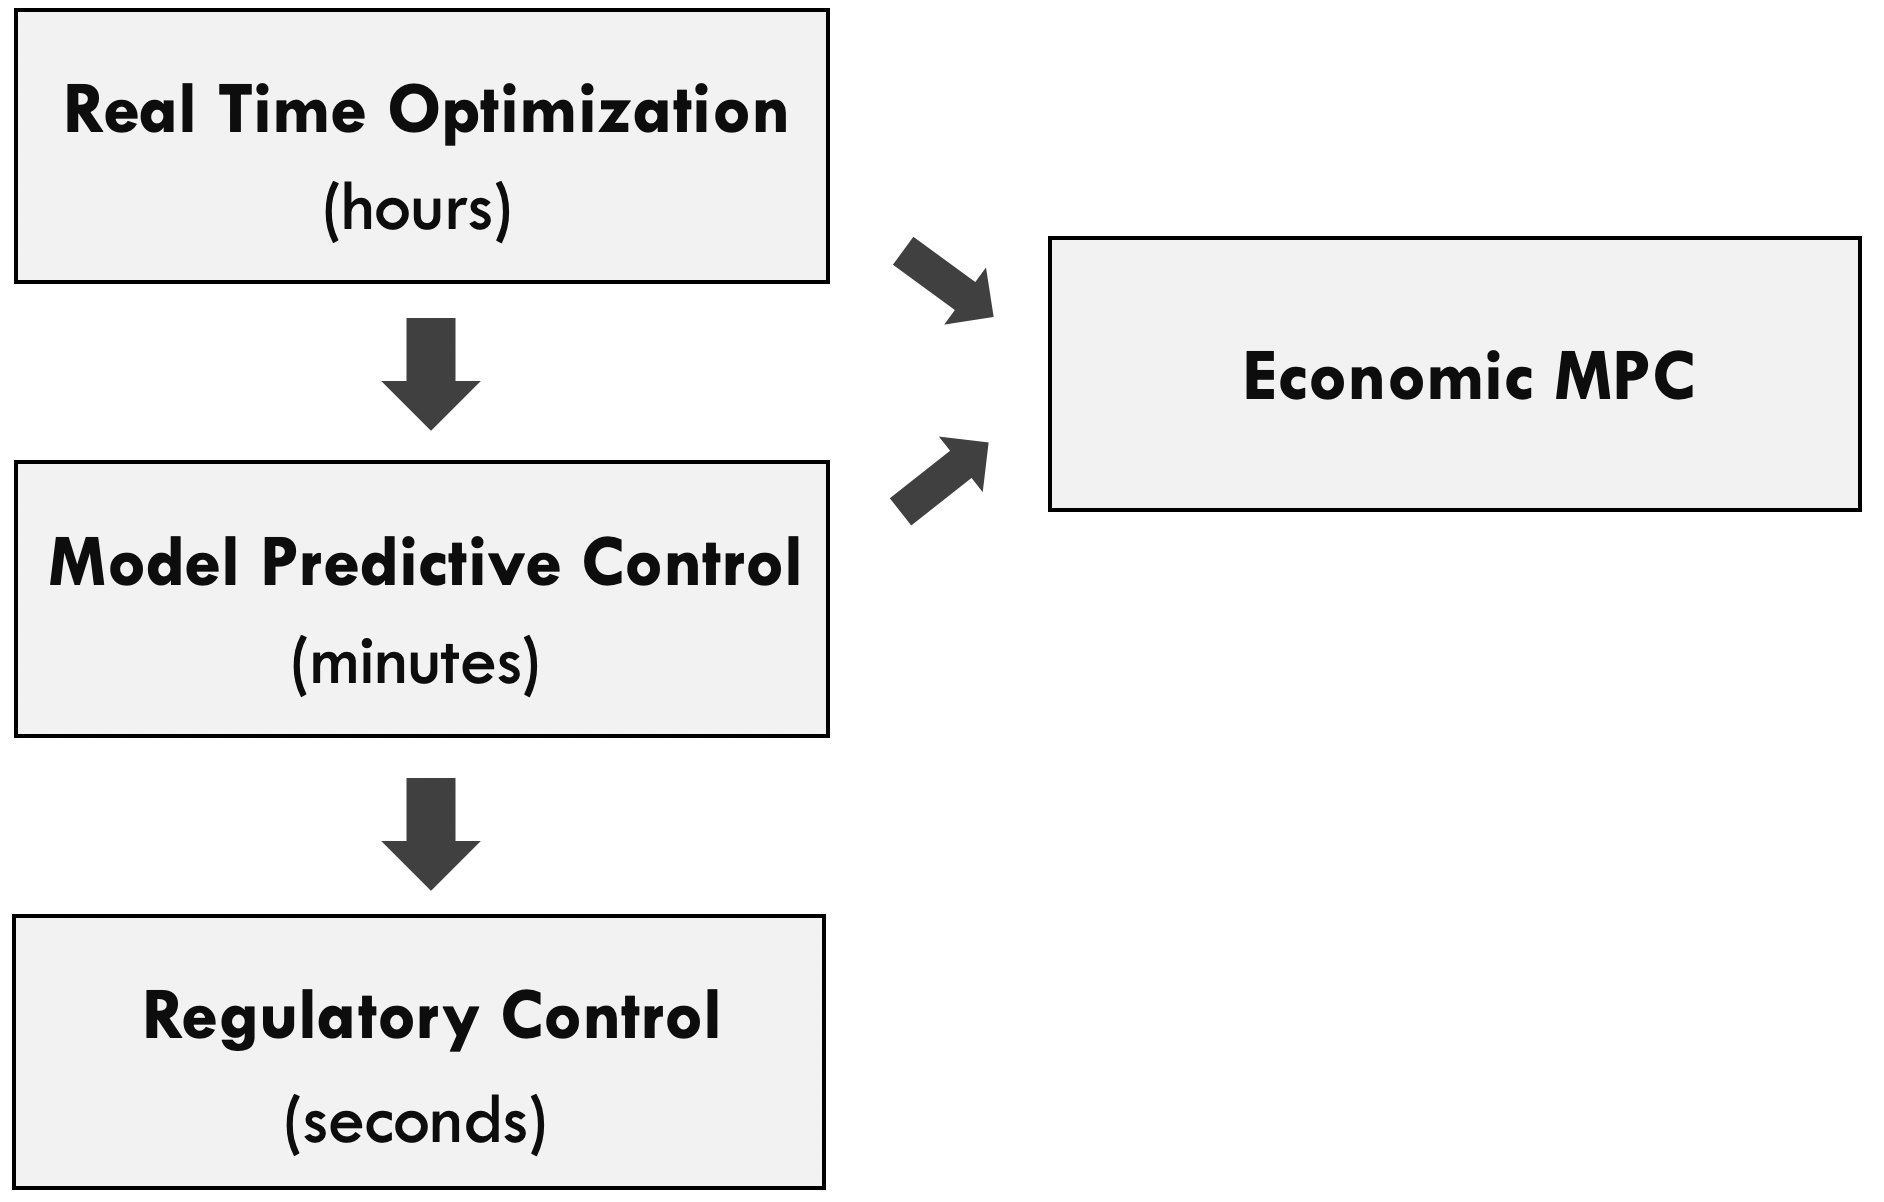
\includegraphics[width=0.5\textwidth]{images/ch1/rto_mpc_pid.jpeg}
    \caption{The traditional control architecture.}
    \label{fig:rto_mpc_pid}
\end{figure}

Comparatively, RL can be described as a general control algorithm and can be used to replace \textit{any} layer in Figure \ref{fig:rto_mpc_pid}. For example, a MPC or PID based RL would have its reward function to be identical as the negative of Equation \ref{eq:mpc_cost}.  In the EMPC case, the reward function of RL would instead be the economic objective.  In Chapter 4, the performance of RL based supervisory controls will be extensively compared to traditional methods on simple and complicated processes. Additionally, the pros and cons of each method will be summarized.


\chapter{Markov Decision Processes}
\section{Markov Decision Processes}
\subsection{Finite Markov Decision Processes}
\subsection{Infinite Markov Decision Processes}

\section{Semi Markov Decision Processes}
\subsection{Semi Markov Decision Processes}
\subsection{Semi Markov Decision Processes for Control}
Do not assume random system transitions and do not assume stationarity over jump.

\section{Partially Observable Markov Decision Processes}


\chapter{Reinforcement Learning}
Reinforcement learning is a goal-directed learning algorithm which continually improves its own performance through interactions with the environment \cite{sutton}. The main objectives of reinforcement learning are to identify hidden structures within the environment and to find the optimal policy (i.e., optimal input trajectory) through guidance from an internal scalar reward (feedback). Two distinct characteristics that deviate reinforcement learning from other methods are its trial \& error search to find the optimal policy, and its ability to identify delayed reward signals. Modern reinforcement learning methods combine principles of optimal control and learning methods together to solve for the optimal control trajectory in an environment.  In this chapter, fundamental reinforcement learning concepts are first introduced.  Then, tabular based methods will be shown.  However, due to the "curse of dimensionality" of high dimensional problems, tabular based approaches fail to bear fruit.  To overcome these issues, deep neural networks will be used for function approximation, and deep reinforcement learning will be introduced.


\section{Introduction to Reinforcement Learning}

Reinforcement learning takes its roots from the \textit{k}-armed bandit problem that has been extensively studied in engineering, psychology, and statistics.  This problem disregards state information, and only worries about solving the optimal actions for \textit{one} specific situation \cite{thompson1, thompson2, robbins, bellman_bandit}.  As a natural extension, Barto, Sutton and Brouwer expanded the idea to multi-situation systems \cite{bartosuttonbrouwer} through associative search, also known as \textit{contextual bandits}. The main objective of this algorithm was to find an optimal policy, $\pi^*(x)$, for each situation.  However, it only concerns the immediate rewards and not the long term consequences. Reinforcement learning was then developed to find the optimal policy for different situations based on immediate reward and the onward trajectory there-forth.  

\subsubsection{\textit{k}-armed Bandit}

The \textit{k}-armed bandit problem provides the fundamentals to understanding modern reinforcement learning.  Here, an agent is present and must choose action $u$ from $\mathcal{U}$, where $\mathcal{U}$ has $k$ choices.  After each action, a scalar reward from a stationary distribution will be returned to the agent as feedback. Favorable actions yield positive rewards, while unfavorable actions return negative rewards. The objective of the agent is to ultimately maximize reward over $N$ steps.  For each action, there is an expected reward called \textit{value}, given by Equation \ref{eq: value}.

\begin{equation}
    \centering
    q_*(u) = \mathbb{E}[R_t | U_t = u]
    \label{eq: value}
\end{equation}
where $u$ is the action taken at time, $t$.  $R_t$ is a scalar reward returned to the agent after action $u$ was performed at time $t$. $R_t$ is drawn from a stationary distribution (typically Gaussian), $R_t \thicksim N(q_*(u), \sigma^2)$. Finally, $q_*(u)$ is the expected reward of taking action, $u$.

The real value is unknown, however, an estimation can be computed and is denoted as $Q_t(a)$.  Given all $Q_t(a)$ is maintained, at any time, one $Q_t(a)$ will be greater than all others.  Picking the action that corresponds to the maximum $Q_t(a)$ is known as \textit{greedy}, and the agent is said to be \textit{exploiting}.  If a non-maximum action is picked, the agent is \textit{exploring} \cite{sutton}.

Action selection based on estimating the value of actions are called \textbf{Action-value methods} \cite{action_value_method}.  At time $t$, the estimate of the value is given by Equation \ref{eq: value_est} \cite{sutton}.

\begin{equation}
    \centering
    Q_t(a) = \
    = \frac{\sum_{i=1}^{t - 1} R_i \mathbbm{1}_{U_i=u}}
    {\sum_{i = 1}^{t - 1} \mathbbm{1}_{U_i = u}}
    \label{eq: value_est}
\end{equation}
where $\mathbbm{1}$ equals 1 if the condition is true, else 0.  $R_i$ is the reward obtained at the $i^{th}$ episode through selecting action, $U_i$.  Intuitively, the numerator is the sum of rewards when action, $u$, was taken prior to $t$.  Likewise, the denominator is the number of times action, $u$, was taken prior to $t$. As $t \rightarrow \infty$, $Q_t(a) \rightarrow q_*(a)$.  Action selection is based on Equation \ref{eq: bandit_action_selection}.

\begin{equation}
    \centering
    A_t = \argmax_a Q_t(a)
    \label{eq: bandit_action_selection}
\end{equation}

However, initial successful episodes may cause the agent to be stuck at local minimums. To overcome this, a semi-stochastic action selection method called $\epsilon$-greedy can be introduced to promote exploration. In this method, the agent will perform a random action with $\epsilon$ probability (greedy action can be performed).  Higher $\epsilon$ results in more exploratory moves.  Consequently, all $u \in \mathcal{U}$ will be picked many times and by the law of large numbers, $Q_t(a) \rightarrow q_*(a)$ \cite{large_numbers}. Figure \ref{fig: eps_figure} shows the effect of $\epsilon$ on the performance of the agent.

\begin{figure}[h]
    \centering
    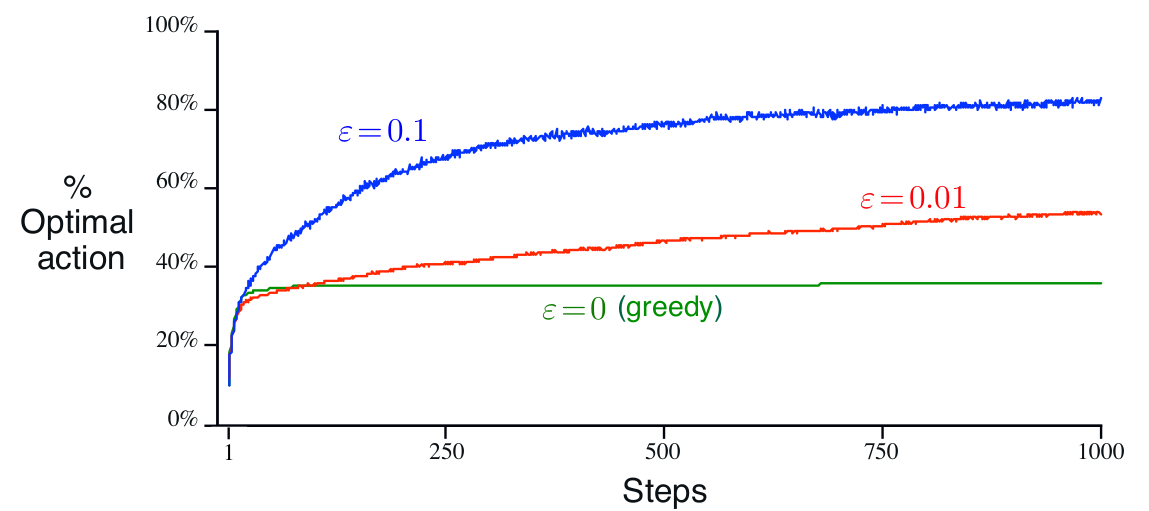
\includegraphics[scale=0.35]{images/eps_vs_optAction.png}
    \caption{Average performance of three agents using different $\epsilon$.  The data is averaged over 2000 runs.  Figure from \textit{Reinforcement Learning: An Introduction} by Sutton and Barto (2018).}
    \label{fig: eps_figure}
\end{figure}

During implementation, $\epsilon$ should decay out as $Q_t(a)$ approaches $q_*(a)$ to ensure knowledge of the agent is being adequately exploited. For non-stationary problems, $\epsilon > 0 \; \forall t$ to ensure other action values have not changed.

Algorithms to solve the \textit{k}-armed bandit problem are easily applied to situations where the concept of state is inert and only the actions are of concern;  a near impossibility in the real world.  

\subsubsection{Contextual Bandit}

A natural extension of the \textit{k}-armed bandit is associative search.  In associative search (sometimes called contextual bandit), different policies are associated with different situations \cite{bartosuttonbrouwer}.  Equation \ref{eq: state-action-value} is the extension of Equation \ref{eq: value} in the associative search problem.

\begin{equation}
    \centering
    q_*(x, u) = \mathbb{E}[R_t | X_t = x, U_t = u]
    \label{eq: state-action-value}
\end{equation}

Associative search is known as the method between \textit{k}-armed bandits and reinforcement learning.  In associative search, the objective is to associate optimal policies to different situations, but only maximizing the \textit{immediate} reward.  Often times, near term sacrifices are required to initiate the trajectory to a large lump sum reward at the terminal state.  For example, heavy capital and time investment is required for University in the short term.  However, the long term gain is so great that it outweighs the short term losses, making going to University an optimal policy for many individuals.

\subsubsection{The Reinforcement Learning Problem}

In order to find the true optimal policy (i.e., policy that returns the greatest rewards over a long time period), the topic of reinforcement learning is developed.  In reinforcement learning, sequential decision making is explored to identify the delayed reward signals from different actions and to ultimately find the optimal policy, $\pi^*$.  

In general terms, reinforcement learning is simply the learning an agent experiences through interactions with the environment.  For added intuition, Figure \ref{fig: simple_rl} shows the generic information flow of reinforcement learning. First, the agent observes some states, $x_t \in \mathcal{X}$, from the environment (some states may be unobservable).  Given $x_t$, the agent performs some actions, $u_t \in \mathcal{U}$ and receives a scalar reward signal, $r_{t+1} \in \mathcal{R}$.  Finally, the environment will transition to a new state, $x_{t+1}$, given probability $P(x_{t+1}, r_{t+1} | x, u)$.

\begin{figure}[h]
    \centering
    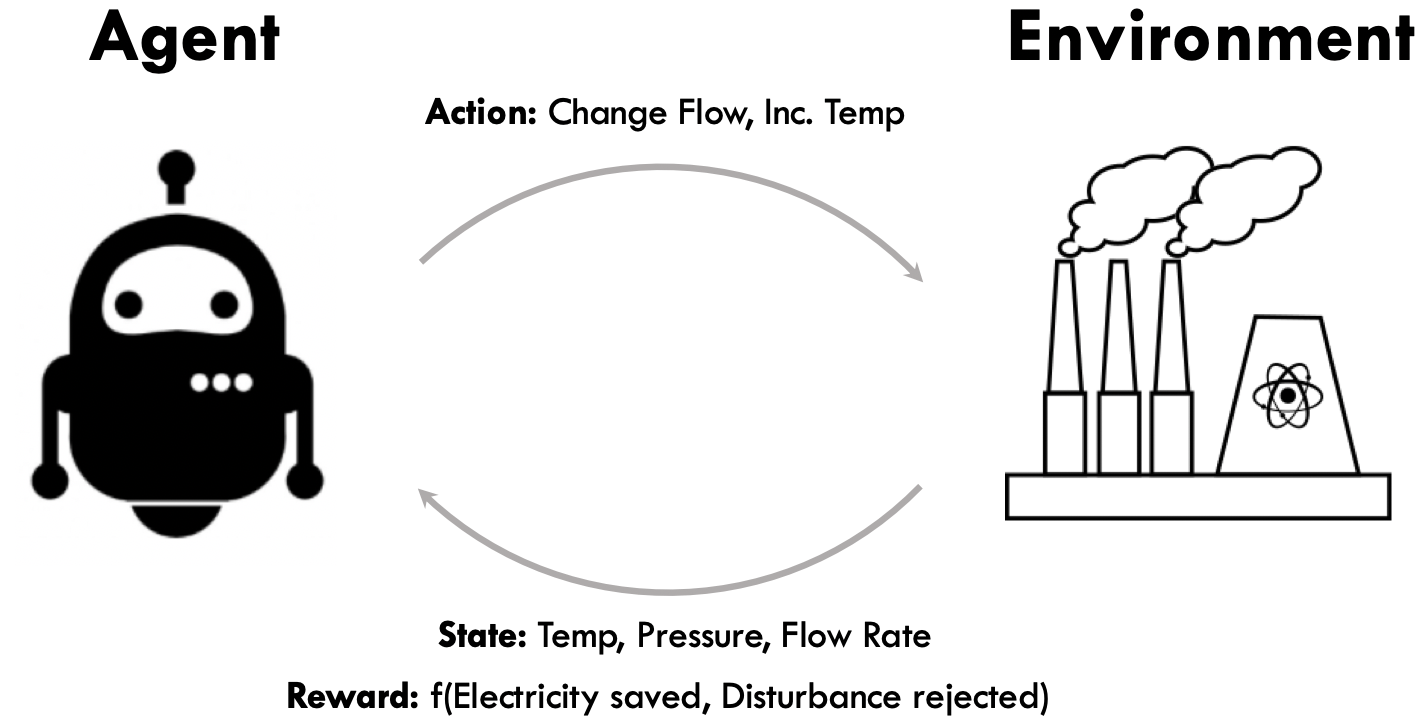
\includegraphics[scale=0.5]{images/RL.png}
    \caption{Basic setup of reinforcement learning where an agent interacts with the environment}
    \label{fig: simple_rl}

\end{figure}

Reinforcement learning consists of the following four elements:

\begin{itemize}
    \item Policy, $\pi$
    \item Reward, $R$
    \item Value Function, $V(s)$
    \item Model (optional), $\dot{x} = Ax + Bu$
\end{itemize}

The policy, $\pi$, of reinforcement learning is a direct mapping from $X \rightarrow U$.  To find the optimal policy, $\pi^*$, the agent is guided by an immediate scalar reward for each interaction (also called \textit{episode}). Policies resulting in higher rewards are more likely to be followed in the future, \textit{mutatis mutandis}.  However, reinforcement learning is concerned with the long term success rather than immediate pleasure. Often times, long term success require short term sacrifice.  Thus, the value function, $V^{\pi}(s)$, is used to describe the long term expected reward under each policy.  Initially, the value function for each state is initialized at zero.  After each episode, the value function will be updated to reflect the new knowledge obtained from the last episode through Equation \ref{eq: value_function}.

\begin{equation}
    \centering
    V(x_t) \leftarrow V(x_t) + \alpha [V(x_{t + 1}) - V(x_t)]
    \label{eq: value_function}
\end{equation}

In Equation \ref{eq: value_function}, $\alpha$ represents the step-size parameter.  That is, how big each update step should be.  Once convergence is achieved for $V(x_t)$, the optimal policy can be described by Equation \ref{eq: opt_policy}.  

\begin{equation}
    \centering
    \pi^*(x) = \argmax_u q_{\pi}(x, u), \; \forall x 
    \label{eq: opt_policy}
\end{equation}

Lastly, reinforcement learning \textit{can} consist of a model. Such cases are called \textit{model-based} reinforcement learning.  The model will be used for planning, and is a way for the agent to plan a control trajectory before they are experienced.  Contrarily, \textit{model-free} reinforcement learning learns \textit{explicitly} through interactions with the environment.

One key topic of reinforcement learning is: \textbf{exploration} vs. \textbf{exploitation}.  At first, the agent must explore to learn the state space, $\mathcal{X}$.  But the agent must know \textit{when} to stop exploring, and start exploiting (i.e., start taking advantage of what is known).  If the agent explores too much, lots of value is lost.  However, if the agent does not explore enough, the current policy may not be optimal and more value is lost long term.  Exploration vs. exploitation is one of the most important topics today in reinforcement learning, and the time to switch from exploration to exploitation will vary between problems.  In control theory, exploration vs. exploitation is known as the conflict between identification (or estimation) and control \cite{explorevexploitcontrol}.  

Another important distinction between different reinforcement learning algorithms is \textbf{on-policy} vs. \textbf{off-policy}.  On-policy methods select actions that maximizes reward given the current knowledge of the agent.  Subsequently, off-policy methods perform exploratory actions for a chance that the explored action offers superior returns to the current best known action.

In the next sub-sections, the three fundamental reinforcement learning methods (Dynamic Programming, Monte Carlo, Temporal-Difference) will be introduced.

\subsection{Dynamic Programming Methods}
\subsubsection{Value-Iteration}
\subsubsection{Policy-Iteration}
\subsection{Monte Carlo Methods}
\subsection{Temporal-Difference Methods}
\subsection{Reinforcement Learning vs. Other "Learnings"}

Machine learning consists of the following four classes: i) Supervised learning, ii) Unsupervised learning, iii) Semi-supervised learning, iv) Reinforcement learning.  Supervised learning is fitting a model to a set of labeled data provided by a subject matter expert.  Subsequently, unsupervised learning is used on unlabeled data sets.  The objective of unsupervised learning is to explore the data and identify hidden features. Semi-supervised learning combines the strengths of supervised and unsupervised learning, and is especially useful \cite{machine_learning}.  Often times, industrial data will be partially labelled due to the time and cost associated with data labelling.  For supervised and unsupervised learning, only the labeled and unlabeled data can be used, respectively.  However, all data can be used in semi-supervised learning which allows for maximized data efficiency and increased model performance. Finally, reinforcement learning is a goal-directed learning from interactions with the environment \cite{sutton}.

Reinforcement learning is a unique class of machine learning.  An ideal supervised learning model can only be as good as the subject matter expert providing the labels to the data set, which may not be 100\%.  For example, in a complex control task, the control law is usually highly non-linear. Control experts can try to provide control strategies for such systems, but optimality may not be guaranteed for highly non-linear systems. Also, supervised learning is used to generalize responses for occurrences not present in the data \cite{sutton}.  Reinforcement learning works by directly interacting with the environment \textit{without labels}. Through adequate exploration, reinforcement learning will identify peculiar features to optimally control such problems [citation required].  Reinforcement learning is \textit{similar} to unsupervised learning in terms of identifying hidden structures within the environment.  However, reinforcement learning tries to maximize an internal scalar "reward" signal, rather than purely data mining.

Evolutionary methods, a family of optimization algorithms such as genetic algorithm, are most similar to reinforcement learning.  For a control problem, such methods can apply multiple static policies for different operating regimes \cite{sutton}.  Policy search is conducted by first initiating $k$ random input trajectories of length $N$, generating input matrix $\mathbb{U}_{[k, N]} \in \pi$.  Subsequently, the loss, $J_U$, of each $U$ is calculated based on the objective function.  Input trajectories with the lowest loss move onto the next generation and generates new pseudo-random input trajectories.  This process is repeated until optimal policy, $\pi^*$ is found for each operating regime \cite{ga_for_control}.

Evolutionary methods work well when the policy space is sufficiently small, easy to find, or a lot of time is available for optimization.  The biggest advantage of such methods compared to reinforcement learning is that the whole state does not need to be known.  However, such methods does not capture the reinforcement learning fundamentals of mapping $X \rightarrow U$.  Unlike evolutionary methods, reinforcement learning keeps memory of each indvidual interaction making it a more data efficient approach \cite{sutton}.

%%%%%%%%%%%%%%%%%%%%%%%%%%%%% End Section Intro to RL %%%%%%%%%%%%%%%%%%%%%%%%%%%%%%%%%%%%%%%


%%%%%%%%%%%%%%%%%%%%%%%%%%%%% Begin Section Tabular RL %%%%%%%%%%%%%%%%%%%%%%%%%%%%%%%%%%%%%%

\section{Tabular Q-learning}
\subsection{Introduction to Q-learning}
\subsubsection{Adaptation to Non-Stationary Problems}
\subsubsection{Incremental Implementation}
\subsubsection{Action Selection}
\subsubsection{Exploration in Tabular Q-learning}
\subsubsection{Reward Functions}
\subsubsection{Expected Returns for Different MDPs}

\subsection{Overall Setup}

%%%%%%%%%%%%%%%%%%%%%%%%%%%%% End Section Tabular RL %%%%%%%%%%%%%%%%%%%%%%%%%%%%%%%%%%%%%%%

%%%%%%%%%%%%%%%%%%%%%%% Begin Section Function Approximation %%%%%%%%%%%%%%%%%%%%%%%%%%%%%%%

\section{Function Approximation}
\subsection{Introduction to Function Approximations}
\subsection{Neural Network Basics}
\subsubsection{Neural Network Initialization}
\subsubsection{Gradient Descent Updating}
\subsubsection{Mini-batch Gradient Descent}
\subsubsection{Batch Normalization}
\subsubsection{Regularizations}

%%%%%%%%%%%%%%%%%%%%%%%%% End Section Function Approximation %%%%%%%%%%%%%%%%%%%%%%%%%%%%%%%


%%%%%%%%%%%%%%%%%%%%%%%%%%%%%%%%% Begin Section DDPG %%%%%%%%%%%%%%%%%%%%%%%%%%%%%%%%%%%%%%%

\section{Deep Deterministic Policy Gradient}
\subsection{Actor-Critic Intuition}
\subsection{Actor - Deterministic Policy Gradient}
\subsection{Critic - Deep Q-learning}

\newpage

\subsection{Exploration in DDPG}
\subsubsection{White Exploratory Noise}
\subsubsection{Ornstein-Uhlenbeck Exploratory Noise}
\subsection{Stabilization of Training}
\subsubsection{Experience Replay}
\subsubsection{Target Network}
\subsubsection{Adaptive Batch Gradient Descent}
\subsubsection{Reward Clipping}
\subsection{Input and State Constraints}
\subsection{Training Algorithm}

%%%%%%%%%%%%%%%%%%%%%%%%%%%%%%%%%% End Section DDPG %%%%%%%%%%%%%%%%%%%%%%%%%%%%%%%%%%%%%%%%


\chapter{Model Predictive Control}
\input{chapters/Chapter04:ModelPredictiveControl.tex}

\chapter{Comparison of RL and MPC}
\input{chapters/Chapter05:ComparisonofRLandMPC.tex}

\chapter{RL for Production Optimization and Alarm Management}
Introduce the problem...

\subsection{Process Introduction}

\subsubsection{Process Description}
\subsubsection{Project Objectives}

\subsection{Supervisory Control using Reinforcement Learning}

\subsection{Alarm Management}

\subsubsection{Alarm Reduction}
\subsubsection{Alarm Prioritization}


\chapter{Imperial Oil: Distillation Flooding Fault-Tolerant Control using RL}
Distillation towers are integral units in industrial processes that require the separation of
mixtures of different components into products based on their relative volatility. Heavy oil
upgrading facilities utilize distillation towers to separate feed mixtures into various products based on their specific gravity.  For many chemical plants, the distillation tower can account up to 50\% of the total operating cost, making optimization of the distillation tower a low hanging fruit in terms of cost savings.  

Flooding is a common and costly problem in industrial distillation towers.  Flooding occurs when liquids are entrained in the vapour due to abnormally high vapour flow rates.  Moreover, the excess pressure also causes liquid holdup in the higher plates of the distillation tower. Ultimately, this leads to significant reduction in separation efficiency causing a loss in production, wasted energy, and off-spec products.

In this chapter, a reinforcement learning based fault tolerant controller will be introduced to mitigate damage caused by flooding events in distillation towers.  The process will first be introduced. Then, common faults will be introduced into the system.  Following that, PID, MPC and RL will all be used to try to guide the system out of the fault situation.  Finally, the performance of each controller will be compared.

\section{Process Introduction}
The Wood-Berry distillation tower, located in the University of Alberta, will be used for this study to compare the performance between PID, MPC, and RL controllers in a fault positive scenario.  

\subsection{Process Description}
Distillation is the process of separating a liquid or vapour mixture of two or more components into desirable purities through the addition or removal of heat. The fundamental theory of distillation is that low boiling point components are richer in the vapour of a boiling mixture, while the liquids would contain more of the less volatile components \cite{distillation_intro}.  Liquids exit the bottom of the distillation tower and is sent to a reboiler, where heat is added to vaporize any straggling high volatility product to ensure maximum separation. Similarly, vapour from the top of the tower is sent to a condenser, where heat is removed and additional low volatility components may be recovered. The condensed vapour is collected in the reflux drum, and will be recycled back into the distillation tower. Typically, distillation columns are large vertical drums with evenly spaced trays to enhance separation of the vapour and liquid components \cite{mpc_for_distillation_tower}.  The tower is separated into two sections.  The rectifying section is located between the feed tray and the top of the column and aims to concentrate light components in the vapour phase.  Moreover, the stripping section is located between the feed tray and the column bottom and is used to concentrate the heavier components in the liquid phase \cite{henry_distillation}.

A process flow diagram of the Wood-Berry tower is shown in Figure \ref{fig: woodberry}.  It contains one feed stream and two outlet streams.  Commonly, the feed stream is characterized by the inlet mol composition, $Z_f$.  The top product, also called distillate, is characterized by mass fraction, $X_D$.  The bottom product is characterized by mass fraction, $X_B$.  The process has two control inputs and two outputs. The control inputs of the system are the reflux and steam flow rates, $R$ and $S$.  The outputs are the distillate and bottoms product mass compositions, $X_D$ and $X_B$.

\begin{figure}[h]
    \centering
    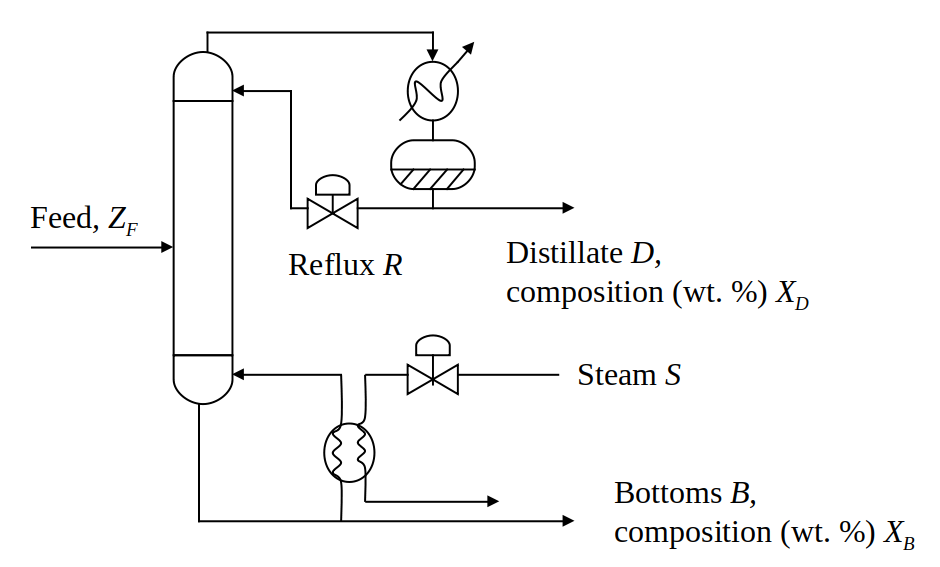
\includegraphics[scale=0.45]{images/woodberry.png}
    \caption{A schematic diagram of a binary distillation tower.}
    \label{fig: woodberry}
\end{figure}

In the Wood-Berry distillation tower, the goal is the complete separation of methanol and water.  Methanol has a boiling point of 64.7 \textdegree C whereas pure liquid water has a boiling point of 100 \textdegree C \cite{sonntag_thermo}. Thus, making methanol the distillate and water is the bottoms product. $X_D$ and $X_B$ are the distillate and bottoms $\%MeOH$, respectively. The two manipulated variables in the system are the reflux flow rate, $R \; (lb/min)$ and the steam flow rate, $S \; (lb/min)$.  The objective of the manipulated variables is to achieve 100\% $X_D$, while maintaining $X_B$ at 0\%. Additional detailed information about the operation and inner workings of distillation towers can be found in \cite{henry_distillation}.  

\subsection{Wood-Berry Models}
The transfer function realization of the Wood-Berry distillation tower is given in Equation \ref{eq: woodberry_tf} \cite{mpc_for_distillation_tower}.

\begin{equation}
    \centering
    \begin{bmatrix}
        Y_1(s) \\
        Y_2(s) 
    \end{bmatrix}
    =
    \begin{bmatrix}
        G_{11}  & G_{12} \\
        G_{21}  & G_{22}
    \end{bmatrix}
    \begin{bmatrix}
        u_1(s) \\
        u_2(s)
    \end{bmatrix}
    \label{eq: woodberry_tf}
\end{equation}
where: 
\begin{equation}
    \centering
        {\large
        \begin{matrix}
            G_{11} = \frac{12.8e^{-s}}{16.7s + 1}     &     G_{12} = \frac{-18.9e^{-3s}}{21s + 1} \\
            G_{21} = \frac{6.6e^{-7s}}{10.9s + 1}     &     G_{22} = \frac{-19.4e^{-3s}}{14.4s + 1}
        \end{matrix}}
    \label{eq: transfer_functions_woodberry}
\end{equation}

Due to the difficulty of transfer function simulations in Python, the model was converted into state space form.  After conversion, two control loops had to be developed to realize the system because of inconsistencies in the input time delay.  Equations \ref{eq: x_ss_eq1} and \ref{eq: x_ss_eq2} are the state space models for the distillate and bottoms compositions, respectively.  The initial states were assumed to be all zero.

\begin{equation}
    \centering
    x_0 = 
    \begin{matrix}
        [0 & 0 & 0 & 0]
    \end{matrix}
\end{equation}

\begin{equation}
    \centering
    \begin{bmatrix}
        \dot{x_1} \\
        \dot{x_2} \\
        \dot{x_3} \\
        \dot{x_4} 
    \end{bmatrix}
    =
    \begin{bmatrix}
        -0.0599     &     0     &     0     &     0 \\
        0           &  -0.0917  &     0     &     0 \\
        0           &     0     &   -0.0476 &     0 \\
        0           &     0     &     0     &  -0.0694
    \end{bmatrix}
    \begin{bmatrix}
        x_1 \\
        x_2 \\
        x_3 \\
        x_4 
    \end{bmatrix}
    +
    \begin{bmatrix}
        1     &     0  \\
        1     &     0  \\
        0     &     1  \\
        0     &     1
    \end{bmatrix}
    \begin{bmatrix}
        u_1(t - 1) \\
        u_2(t - 3)
    \end{bmatrix}
    \label{eq: x_ss_eq1}
\end{equation}

\begin{equation}
    \centering
    X_D(t) =  
    \begin{matrix}
        [0.7665 & 0 & -0.9 & 0]
    \end{matrix}
    \begin{matrix}
        [x_1 & x_2 & x_3 & x_4]^T
    \end{matrix}
    \label{eq: X_D_output}
\end{equation}

\begin{equation}
    \centering
    \begin{bmatrix}
        \dot{x_1} \\
        \dot{x_2} \\
        \dot{x_3} \\
        \dot{x_4} 
    \end{bmatrix}
    =
    \begin{bmatrix}
        -0.0599     &     0     &     0     &     0 \\
        0           &  -0.0917  &     0     &     0 \\
        0           &     0     &   -0.0476 &     0 \\
        0           &     0     &     0     &  -0.0694
    \end{bmatrix}
    \begin{bmatrix}
        x_1 \\
        x_2 \\
        x_3 \\
        x_4 
    \end{bmatrix}
    +
    \begin{bmatrix}
        1     &     0  \\
        1     &     0  \\
        0     &     1  \\
        0     &     1
    \end{bmatrix}
    \begin{bmatrix}
        u_1(t - 7) \\
        u_2(t - 3)
    \end{bmatrix}
    \label{eq: x_ss_eq2}
\end{equation}

\begin{equation}
    \centering
    X_B(t) =  
    \begin{matrix}
        [0 & 0.6055 & 0 & -1.3472]
    \end{matrix}
    \begin{matrix}
        [x_1 & x_2 & x_3 & x_4]^T
    \end{matrix}
    \label{eq: X_B_output}
\end{equation}

\subsection{Model Validation}

To ensure the state space model is equivalent to the original transfer function model, step tests were conducted on both systems.  The input for $u_1$ and $u_2$ were set to 1 for 150 time steps and the output trajectory is shown in Figure \ref{fig: step_test_plots} for both the transfer function and state space models. From Figure \ref{fig: step_test_plots}, it can be seen that both trajectories are identical. 

\begin{equation}
    \centering
    u_t = 
    \begin{bmatrix}
        1  &  1  &  ...  &  1 \\
        1  &  1  &  ...  &  1
    \end{bmatrix}_{2 \times N}
    \; where \; N = 150
    \label{eq: step_test_input}
\end{equation}

\begin{figure}[h]
    \centering
    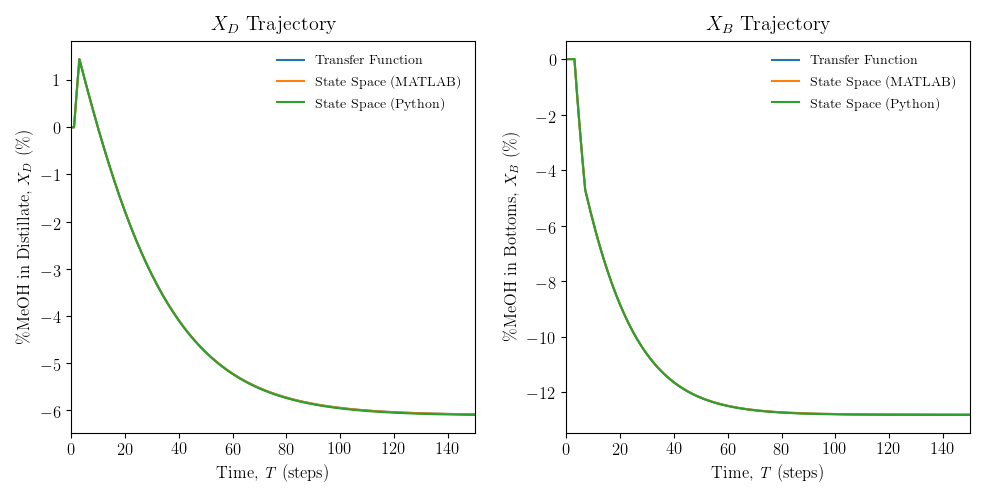
\includegraphics[scale=0.42]{images/step_test_plots.png}
    \caption{A comparison of the $X_D$ and $X_B$ trajectories for the transfer function and state space models}
    \label{fig: step_test_plots}
\end{figure}

To further confirm the validity of the results, the steady state problem was also calculated to ensure simulations were giving correct results. During steady state, the change in states, $\dot{x_i}$, are zero.

\begin{equation}
    \centering
    \dot{x_1}, \dot{x_2}, \dot{x_3}, \dot{x_4} = 0
\end{equation}

Given that $u_1$ and $u_2$ are one (from Equation \ref{eq: step_test_input}), all states can be analytically solved.  Delays will be omitted because the inputs are assumed to be identical for 150 time steps. Equations \ref{eq: x1_analytical} - \ref{eq: x4_analytical} shows the numerical solution to each state at steady state.

{\setstretch{0.5}
\begin{equation}
    \centering
    x_1 = 16.7
    \label{eq: x1_analytical}
\end{equation}

\begin{equation}
    \centering
    x_2 = 10.9
    \label{eq: x2_analytical}
\end{equation}

\begin{equation}
    \centering
    x_3 = 21.0
    \label{eq: x3_analytical}
\end{equation}

\begin{equation}
    \centering
    x_4 = 14.4
    \label{eq: x4_analytical}
\end{equation}
}

Combining Equations \ref{eq: X_D_output} and \ref{eq: X_B_output} with Equations \ref{eq: x1_analytical} - \ref{eq: x4_analytical}, the steady state values for $X_D$ and $X_B$ are given by Equations \ref{eq: final_xd} and \ref{eq: final_xb}, respectively. \\

{\setstretch{0.5}
\begin{equation}
    \centering
    X_D = 0.767x_1 - 0.900x_3
\end{equation}

\begin{equation}
    \centering
    X_D = 0.767(16.7) - 0.900(21.0) = -6.1
    \label{eq: final_xd}
\end{equation}

\begin{equation}
    \centering
    X_B = 0.606x_2 - 1.35x_4
\end{equation}

\begin{equation}
    \centering
    X_B = 0.606(10.9) - 1.35(14.4) = -12.8
    \label{eq: final_xb}
\end{equation}
}

Comparing the analytical steady state solutions found for $X_D$ and $X_B$ to the final steady state values reached in Figures \ref{fig: step_test_plots} it can be seen that the solutions are identical; further confirming the models validity.

\section{Finding the Optimal Solution}

The optimal solution for the Wood-Berry distillation column is given by Equations \ref{eq: xd_optimal} and \ref{eq: xb_optimal}, i.e., perfect separation of methanol from water. To obtain the ideal steady state inputs, $u_1^*$ and $u_2^*$, Equations \ref{eq: final_xd} and \ref{eq: final_xb} are solved with the conditions:

{\setstretch{0.5}
\begin{equation}
    \centering
    X_D^* = 100
    \label{eq: xd_optimal}
\end{equation}

\begin{equation}
    \centering
    X_B^* = 0
    \label{eq: xb_optimal}
\end{equation}
}

By solving Equations \ref{eq: X_D_output} and \ref{eq: X_B_output} for $x_1, x_2, x_3$ and $x_4$ when delays are omitted and $\dot{x}_i$ are zero, the following equations are obtained: \\

{\setstretch{0.5}
\begin{equation}
    \centering
    x_1 = 16.7u_1
    \label{eq: x_1_ss_opt}
\end{equation}

\begin{equation}
    \centering
    x_2 = 10.91u_1
\end{equation}

\begin{equation}
    \centering
    x_3 = 21.0u_2
\end{equation}

\begin{equation}
    \centering
    x_4 = 14.4u_2
    \label{eq: x_4_ss_opt}
\end{equation}
}

Combining Equations \ref{eq: x_1_ss_opt} - \ref{eq: x_4_ss_opt} with \ref{eq: final_xd} and \ref{eq: final_xb}, the optimal inputs are analytically solved and are given by: \\

{\setstretch{0.5}
\centering
$X_D^* = 0.767(16.7)u_1 - 0.900(21.0)u_2$

\begin{equation}
    \centering
    100 = 12.8u_1 - 18.9u_2
    \label{eq: opt_xd}
\end{equation}
}

{\setstretch{0.5}
\centering
$X_B^* = 0.606(10.9)u_1 - 1.347(14.4)u_2$

\begin{equation}
    \centering
    0 = 6.6u_1 - 19.5u_2
    \label{eq: opt_xb}
\end{equation}
}

Combining Equations \ref{eq: opt_xd} and \ref{eq: opt_xb}, the optimal steady state inputs are: \\

{\setstretch{0.5}
\begin{equation}
    \centering
    u_{1, ss}^* = 15.7
\end{equation}

\begin{equation}
    \centering
    u_{2, ss}^* = 5.3
\end{equation}
}

\subsubsection{Simulating the Optimal Solution}
Figures \ref{fig: optimal_ss_xd_xb} show the trajectories of $X_D$ and $X_B$ given the optimal control input.

\begin{figure}[h]
     \centering
      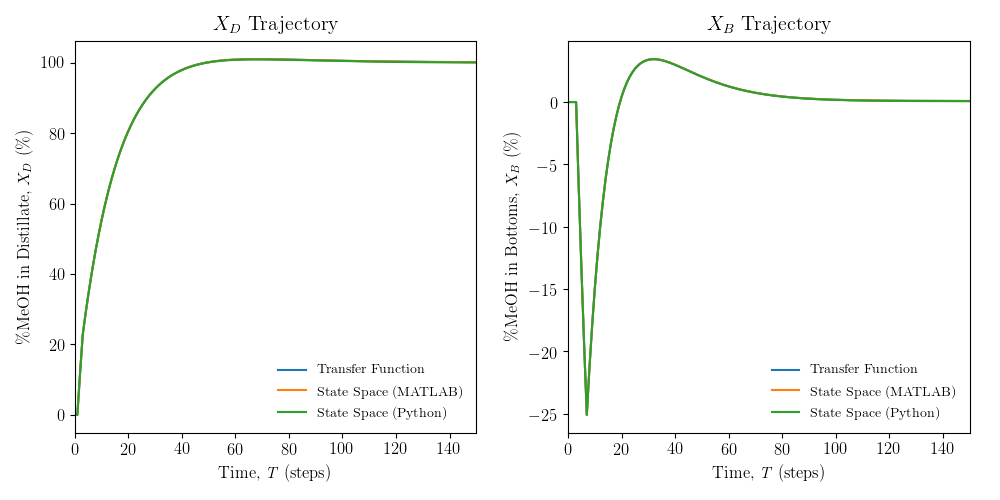
\includegraphics[scale=0.42]{images/optimal_input_plots.png}
     \caption{Trajectories of $X_D$ and $X_B$ using optimal steady state inputs, $u_{ss}^*.$}
     \label{fig: optimal_ss_xd_xb}
\end{figure}

\section{Design of the Control System}
Controllers must first be designed to control the system to desired set-points.  Given that the system has multiple inputs and multiple outputs (MIMO), two different control designs can be explored.  The first control design is building one multi-variate controller capable of controlling both inputs, given feedback from both outputs.  The second design decomposes the system into smaller sub-systems so multiple single-input single-output (SISO) controllers can be applied for control.  In this study, two SISO PID controllers will be designed for regulatory control.  Then, a model predictive controller (MPC) will be designed as a multi-variate supervisory controller.  

\subsection{Relative Gain Array}
Due to the MIMO system being coupled (i.e, the control signal sent to one actuator will indirectly affect the output signal of the second control loop), the relative interactions between the control actions needs to be explored. Exploration of the coupling effect is required to tune the control system appropriately and ensure instabilities do not exist. One simple way to investigate the degree of coupling is to compute the relative gain matrix, $\Lambda$. Using the relative gain matrix, the proper input output pairing can also be determined \cite{RGA}. A flaw in the relative gain array is the lack of consideration for time delays.  However, the PID controllers will be evaluated every 10 seconds, so the effect of delays are assumed to be negligible.  To solve for the relative gains, the process gain, $K_{process}$, for each transfer function in the system must first be identified.  The definition of $K_{process}$ is given in Equation \ref{eq: process_gain}:

\begin{equation}
    \centering
    K_{process} = \frac{\partial y_i}{\partial u_i} \approx \frac{\varDelta y_i}{\varDelta u_i}
    \label{eq: process_gain}
\end{equation}
where $\partial y_i$ and $\partial u_i$ are the partial derivative of the outputs and inputs, respectively. The function can be approximated by the change in $y_i$ and $u_i$, given the step sizes are sufficiently small.  Intuitively, $K_{process}$ describes the relative effect of $u_i$ on $y_i$.  

The standard form of a transfer function is given by:

\begin{equation}
    \centering
    G(s) = \frac{Y(s)}{U(s)} = \frac{K}{\tau s + 1}
\end{equation}
where $K$ and $\tau$ are the process gain and time constant, respectively.

Referring to Equation \ref{eq: transfer_functions_woodberry}, all the transfer functions are in standard form.  Therefore, their process gains are simply the coefficient of the numerators and are:

\begin{equation}
    \centering
    K_{ij} =
    \begin{bmatrix}
    12.8     &     -18.9 \\
    6.6      &     -19.4 
    \end{bmatrix}
    \label{eq: process_gains}
\end{equation}
where $i$ denotes the $i^{th}$ element in each row and $j$ denotes the $j^{th}$ element in each column (e.g. $K_{18}$ denotes the element in the first row and 8th column).

The general form of the system outputs is:

\begin{equation}
    \centering
    \begin{bmatrix}
        y_1 \\
        y_2
    \end{bmatrix}
    =
    \begin{bmatrix}
        K_{11}  &  K_{12} \\
        K_{21}  &  K_{22}
    \end{bmatrix}
    \begin{bmatrix}
        u_1 \\
        u_2
    \end{bmatrix}
    \label{eq: general_ss_form}
\end{equation}
where $y_1$ and $y_2$ are the system outputs.  Subsequently, $u_1$ and $u_2$ are the system inputs. \\

\noindent
The standard form of Equation \ref{eq: general_ss_form} is:
{\setstretch{0.5}
\begin{equation}
    \centering
    y_1 = K_{11}u_1 + K_{12}u_2
    \label{eq: y1_iol}
\end{equation}
\begin{equation}
    \centering
    y_2 = K_{21}u_1 + K_{22}u_2
    \label{eq: y2_iol}
\end{equation}}

\noindent
The relative gain between $y_i$ and $u_j$, $\lambda_{ij}$, is given by:

\begin{equation}
    \centering
    {\Large
    \lambda_{ij} = \frac{(\frac{\partial y_i}{\partial u_j})|_{U}}{(\frac{\partial y_i}{\partial u_j})|_{Y}}
    }
    \label{eq: relative_gain}
\end{equation}
where $U = \mathcal{U}, U \neq u_j$ and $Y = \mathcal{Y},Y \neq y_i$.  The numerator and denominator of the relative gain represents the open loop and closed loop gain between $y_i$ and $u_j$, respectively.

\noindent
Solving for the numerator of $\lambda_{11}$ yields:
\begin{equation}
    \centering
    \left.\frac{\partial y_1}{\partial u_1} \right \vert_{u_2} = \frac{\partial}{\partial u_1}[K_{11}u_1 + K_{12}u_2] = K_{11}
\end{equation}

\noindent
Similarly, solving for the denominator of Equation \ref{eq: relative_gain} gives:
\begin{equation}
    \centering
    \left.\frac{\partial y_1}{\partial u_1}\right\vert_{y_2} = \frac{\partial}{\partial u_1}[K_{11}u_1 + K_{12}u_2]
    \label{eq: y2_relative_gain}
\end{equation}
Since $y_2$ does not appear in Equation \ref{eq: y1_iol}, Equation \ref{eq: y2_iol} must be substituted into Equation \ref{eq: y1_iol}.  Because $y_2$ is a deviation variable, $y_2 = 0$ giving:

\begin{equation}
    \centering
    0 = K_{21}u_1 + K_{22}u_2
    \label{eq: u2_relative_gain1}
\end{equation}
solving for $u_2$:
\begin{equation}
    \centering
    u_2 = \frac{-K_{21}u_1}{K_{22}}
    \label{eq: u2_relative_gain2}
\end{equation}

\noindent
Substituting Equation \ref{eq: u2_relative_gain2} into Equation \ref{eq: y2_relative_gain} and solving the partial derivative yields:

\begin{equation}
    \centering
        (\frac{\partial y_1}{\partial u_1})_{y_2} = \frac{\partial}{\partial u_1}[K_{11}u_1 - \frac{K_{12}K_{21}u_1}{K_{22}}] = K_{11} - \frac{K_{12}K_{21}}{K_{22}}
\end{equation}
The relative gain array, $\Lambda$, is:

\begin{equation}
    \centering
    \Lambda = 
    \begin{bmatrix}
    \lambda_{11}   &   \lambda_{12}   \\
    \lambda_{21}   &   \lambda_{22}
    \end{bmatrix}
\end{equation}
and satisfies the following conditions given $\Lambda$ is a square matrix:
{\setstretch{0.5}
\begin{equation}
    \centering
    \sum_{j = 1}^N \lambda_{ij} = 1
\end{equation}
\begin{equation}
    \centering
    \sum_{i = 1}^M \lambda_{ij} = 1
\end{equation}
\begin{equation}
    \centering
    \lambda_{ij} = \lambda_{ji}
\end{equation}}
where N and M are the number of elements in the rows and columns, respectively.

\noindent
Using the above conditions, the relative gain matrix can be simplified to:
\begin{equation}
    \centering
    \begin{bmatrix}
     K_{11} - \frac{K_{12}K_{21}}{K_{22}}   &   1 - K_{11} - \frac{K_{12}K_{21}}{K_{22}}   \\
     1 - K_{11} - \frac{K_{12}K_{21}}{K_{22}}   &   K_{11} - \frac{K_{12}K_{21}}{K_{22}}
    \end{bmatrix}
    \label{eq: final_relative_gain_array}
\end{equation}
Substituting values from Equation \ref{eq: process_gains} into Equation \ref{eq: final_relative_gain_array} results in:
\begin{equation}
    \centering
    \Lambda = 
    \begin{bmatrix}
     2   &   -1   \\
     -1  &    2
    \end{bmatrix}
    \label{eq: relative_gain_array_w_values}
\end{equation}

The physical meaning of the relative gains are summarized in Table \ref{tab: relative_gains} \cite{process_control_design_sim}.
\begin{table}[h]
    \centering
    {\setstretch{1.5}
    \begin{tabular}{ c | p{12cm} }
        Magnitude of $\lambda_{ij}$  & Physical Meaning \\
        \hline
        $\lambda_{ij} = 1$ & Open and closed loop gains are identical; no interaction effects for pairing $y_i$ and $u_j$ \\
        $\lambda_{ij} = 0$ & Open loop gain is zero; $u_j$ has no effect on $y_i$ \\
        $ 0 < \lambda_{ij} < 1$ & Closed loop interactions increases gain \\
        $\lambda_{ij} > 1$ &  Closed loop interactions reduce gain \\
        $\lambda_{ij} < 0$ & Open and closed loop gains have opposing effects \\
    \end{tabular}}
    \caption{Description of relative gain values.}
    \label{tab: relative_gains}
\end{table}

From $\Lambda$, $\lambda_{12}$ is negative, meaning that pairing $y_1$ with $u_2$ results in opposing open and closed loop gains.  A similar outcome can be seen by pairing $y_2$ with $u_1$.  Both scenarios should be avoided to ensure stability in the system. From Table \ref{tab: relative_gains}, $\lambda_{11}, \lambda_{22} = 2$.  Although this is better than the relative gain being negative, it is still far from 1, so a decoupler should be implemented to achieve independent control of $y_1$ and $y_2$ using $u_1$ and $u_2$.

\subsection{Simple Decoupling using Equivalent Transfer Functions}
In literature, there are three popular decoupling methods: i) ideal, ii) simplified, and iii) inverted [Cite].  The ideal decoupling method requires inversing of the transfer functions, and leads to modelling errors [Cite].  The simplified method overcomes these shortcomings, however, the decoupled process cannot be directly used for controller design without the model reduction technique [Cite].  The inverted method combines all the advantages of the ideal and simplified methods, but high dimensional systems may be physically unrealizable, and it is also more prone to errors [cite].  Rajapandiyan et al. (2012) proposed a new method to perform decoupling of systems with time delays that improve upon the classical methods.  

First, the multi-loop system is decoupled into multiple single loop systems using the simplified decoupler matrix.  The decoupled process is then approximated using its effective open-loop transfer function (EOTF).  Subsequently, Rajapandiyan et al. (2012) showed that the EOTF was exactly equivalent to the equivalent transfer function (ETF) when the system is open-loop stable and there are no oscillatory characteristics.  From the EOTFs, the decentralized PID controllers can then be designed using the simplified internal model control (SIMC) method. 

Referring to Equation \ref{eq: woodberry_tf}, it can be seen that the Wood-Berry distillation system is open-loop stable because all poles are in the left-half plane.  From Figure \ref{fig: step_test_plots}, the system also has no oscillations during step tests. Thus, the system in this study satisfies the requirements posed by Rajapandiyan et al. (2012). 

\subsubsection{Decoupler Design}
Figure \ref{fig: control_loop_IOL} shows the simplified closed-loop control system for the Wood-Berry distillation tower \cite{decoupler_design}.  $G_c(s)$ and $G(s)$ are the distributed controller matrix and the process transfer functions, respectively, and are shown in Equations \ref{eq: transfer_functions_woodberry} and \ref{eq: controller_tf_iol}.  $y_{r_1}$ and ...

\begin{figure}
    \centering
    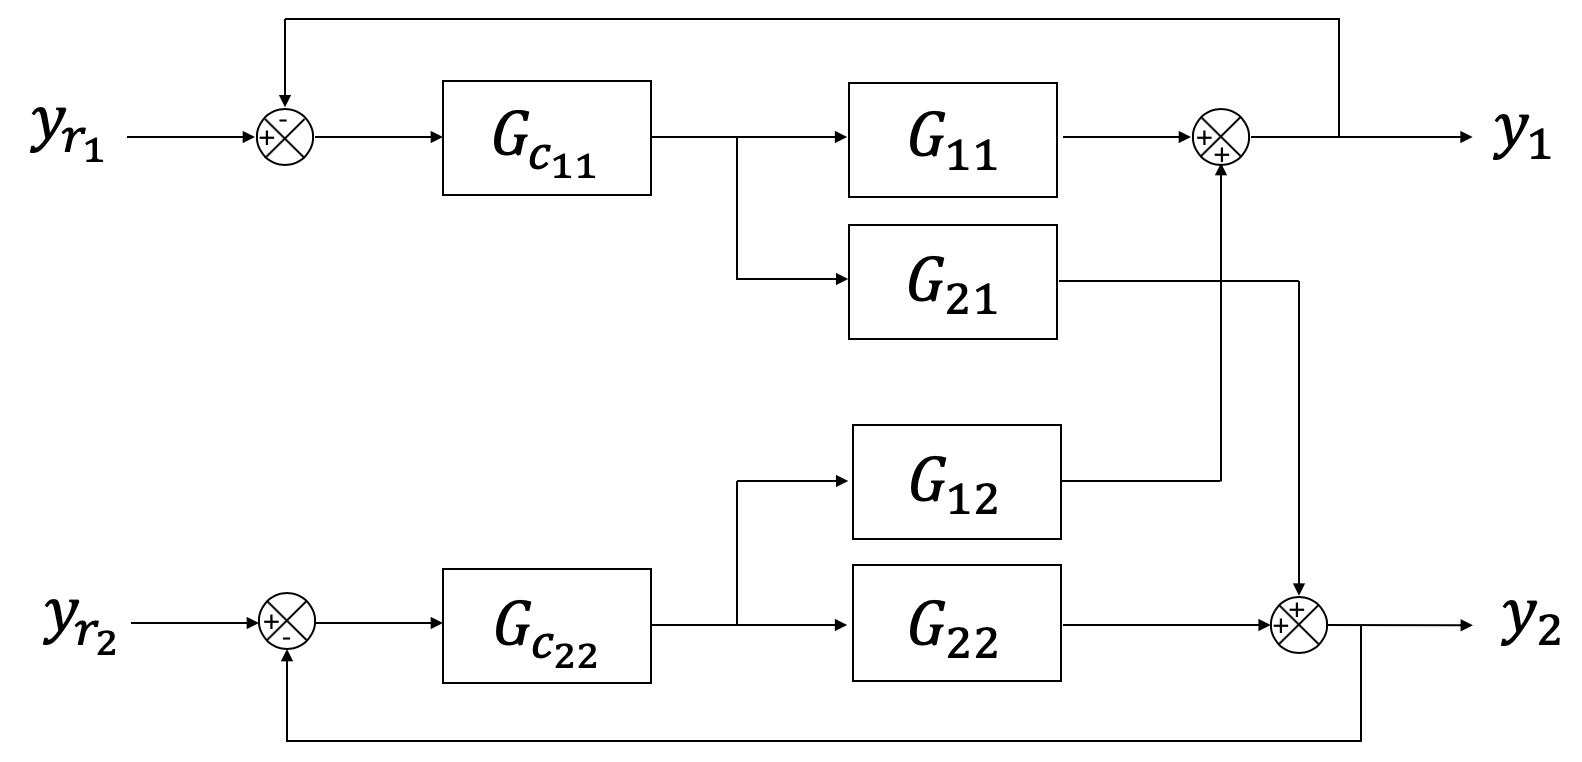
\includegraphics[scale=0.45]{images/pid_loop_iol.png}
    \caption{Simplified control system of the Wood-Berry distillation tower.}
    \label{fig: control_loop_IOL}
\end{figure}

\begin{equation}
    \centering
    G_{c}(s) = 
    \begin{bmatrix}
    g_{c_{11}}  &  0 \\ 
    0         &  g_{c_{22}}
    \end{bmatrix}
    \label{eq: controller_tf_iol}
\end{equation}

\begin{figure}[h]
    \centering
    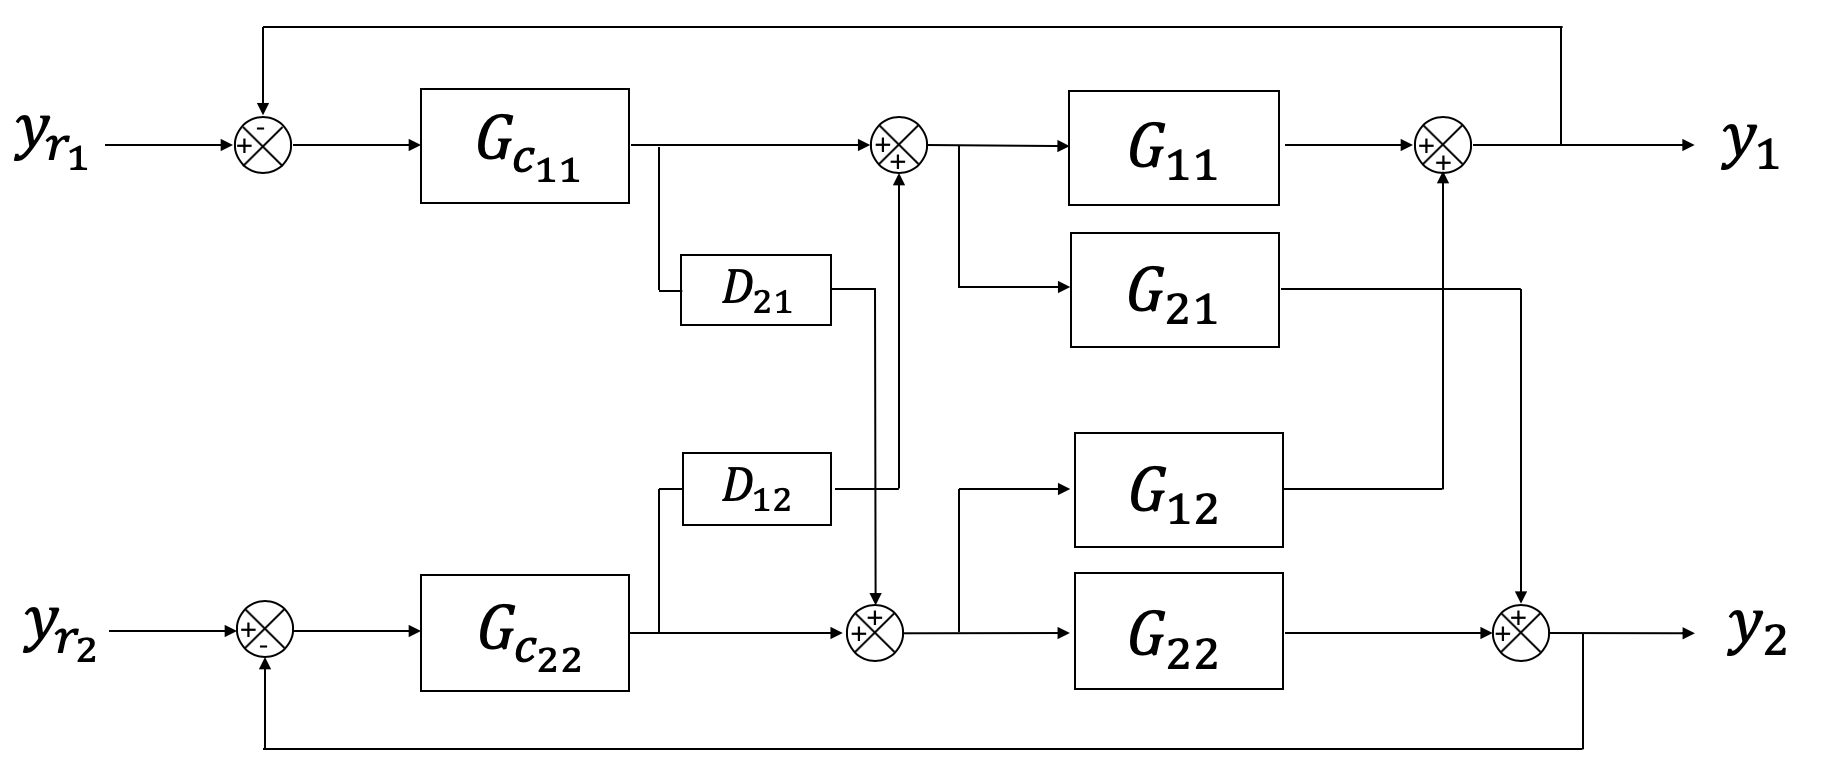
\includegraphics[scale=0.39]{images/decoupled_pid_loop_iol.png}
    \caption{Simplified decoupled control system of the Wood-Berry distillation tower.}
    \label{fig: decoupled_control_loop_IOL}
\end{figure}

\section{Introduction to Fault Tolerant Control}

Inevitably, all process equipment such as sensors, actuators, pumps, will malfunction or break down along their operational lifetime. Therefore, it is desirable to to have a fault tolerant control system (FTCS) in place to accommodate for these inevitable failures and ensure an acceptable level of performance during such events. The application of FTCS in the industrial environment results in increased operation robustness, production, and safety. The complete fault tolerant control system requires two algorithms: i) Fault prediction system to identify the location and type of fault. ii) Fault tolerant controller to "safe land" the process during a fault positive situation \cite{process_faults}.  This particular study is only concerned with the fault tolerant controller design, and assumes that the fault is appropriately identified using existing methods.

One area identified for potential reinforcement learning application is in the design of a fault tolerant controller.  Fault tolerant controllers activate when a process fault occurs, rendering normal controllers useless [citation required]. The objective of fault tolerant controllers are to guide the process out of the fault situation safely.  Subsequently, process engineers can diagnose the problem and re-activate the normal process controllers when deemed acceptable.  

Farivar and Ahmadabadi (2015) has designed fault tolerant controllers using reinforcement learning for a class of unknown linear systems \cite{ahmad}.  Zhang and Gao (2018) applied reinforcement learning fault tolerant controllers to flux cored wired systems \cite{zhang_gao}.  In this project, a reinforcement learning fault tolerant controller will be built for the mitigation of flooding in an industrial distillation tower. 

\section{Controlling using PID}
A PI controller was selected instead of a P or PID controller, because PI controllers are shown to achieve superior control performances compared to their counterparts \cite{PI_controller}.

\section{Controlling using MPC}
\section{Controlling using Reinforcement Learning}
\section{Comparison of Performance}

\chapter{Anomaly Detection and Cost Optimization of a Pipeline}
Pipelines are critical for safe and efficient transportation of fluids across long distances.  For example, pipelines are used by utility companies to transport clean water and natural gas to homes for heating and living purposes.  Furthermore, pipelines are also used in agriculture to transport irrigation water to hydrate crops.  Moreover, pipelines are used by energy companies for transporting energy-rich hydrocarbons to fuel the world's transportation and manufacturing needs. In the United States, over 70\% of petroleum products are shipped by pipeline.  In Canada, the number increases to 97\% \cite{pipeline_transport}.  Data in 2014 estimates that there are approximately 3,500,000 kms of operational pipelines across 120 countries \cite{CIA_pipeline}. Due to the world's dependency on pipelines for transporting their basic needs, ensuring its reliability and efficiency has a global-scale impact.

Typical pipelines have hundreds of digital measurements per minute and are hard to analyze; however, machine learning methods benefit greatly from large amounts of data. Thus, an opportunity was discovered where machine learning methods will be applied to pipelines used to transport petroleum products. The objectives of this project were to leverage machine learning to identify anomalous pipeline behaviour, and to build a real time optimization tool to automate, normalize and enhance pipeline operation.

In this chapter, a time-series neural network classifier will first be introduced to detect anomalous activity within any pipeline equipment. Then, a real time optimization tool based on a linear parameter-varying model will be introduced.  Due to confidentiality agreements, all data presented here-forth will be normalized, and all parties of this project will remain anomalous.

\section{Process Introduction}
Two separate pipelines, Line 11 and Line RM06A, were analyzed.  Line 11 is a simplistic pipeline with few operating variables. Due to the lack of operational flexibility, the data was only able to be leveraged for an anomaly detection tool.  Line RM06A was more complex and had many degrees of freedom. Due to the additional complexity, a real time optimization tool was built for this line.

\subsection{Line 11}
The schematic of Line 11 is shown in Figure \ref{fig:08Line11}. For Line 11, the objective was to build an anomaly detection tool to predict unexpected shut downs of its pumps.  

\begin{figure}[h]
    \centering
    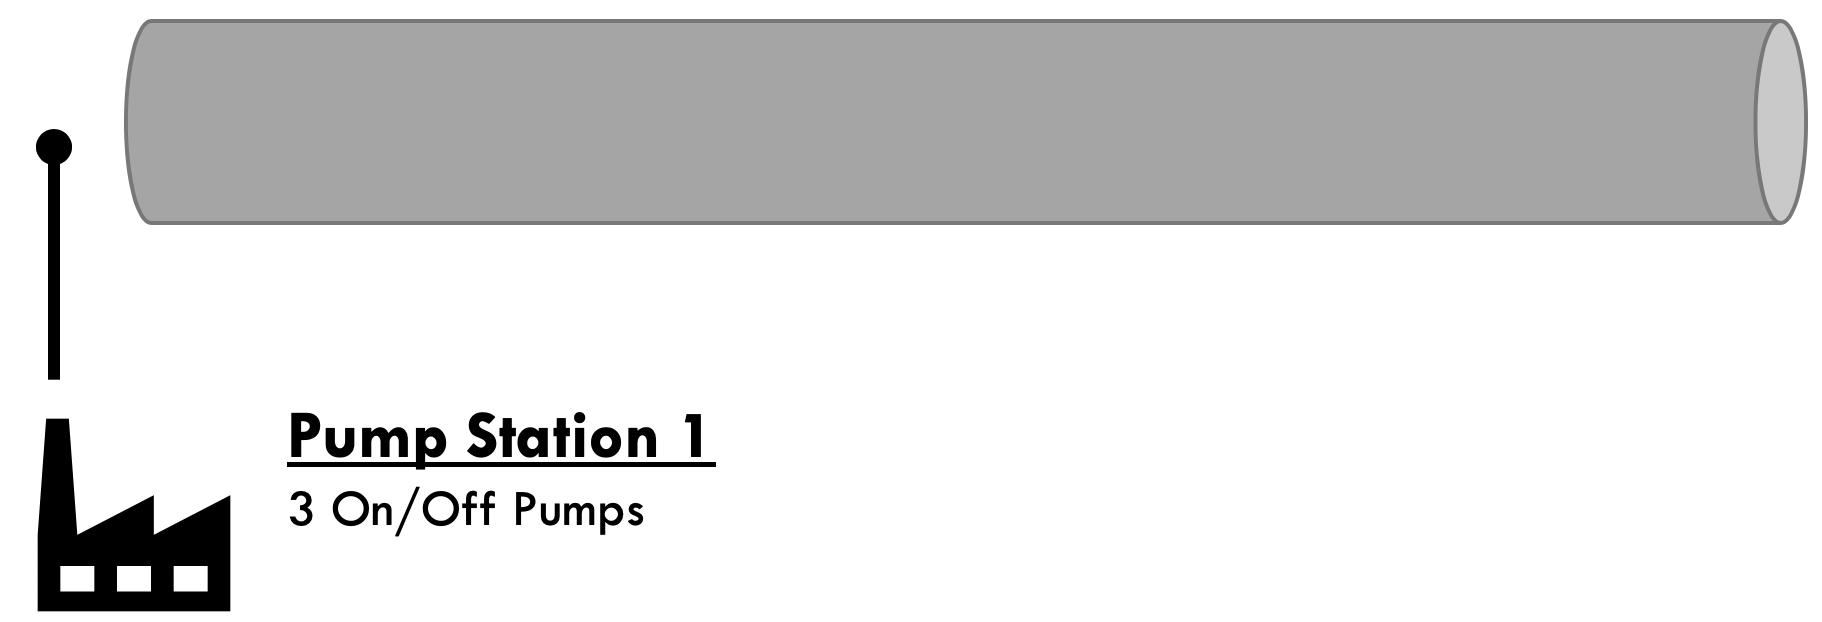
\includegraphics[scale=0.45]{images/08Line11.png}
    \caption{Schematic diagram of Line 11.}
    \label{fig:08Line11}
\end{figure}


\subsection{Line RM06A}
A schematic of line RM06A is shown in Figure \ref{fig:08RM06A}.  Line RM06A is a complex pipeline spanning 151 km and carries two products, a lighter sweet product and a heavier sour product. The two products are batched (i.e., rotate between sending each product) and each product is sent for approximately eight hours before switching to the other product. The American Petroleum Institute (API) gravity for the lighter and heavier products are roughly 40 and 20, respectively. For the rest of this chapter, the lighter and heavier product will be referred to as \textit{sweet crude} and \textit{sour crude}, respectively. The pipeline is typically operated between 1500 bbl/h to 3050 bbl/h. 

\begin{figure}[h]
    \centering
    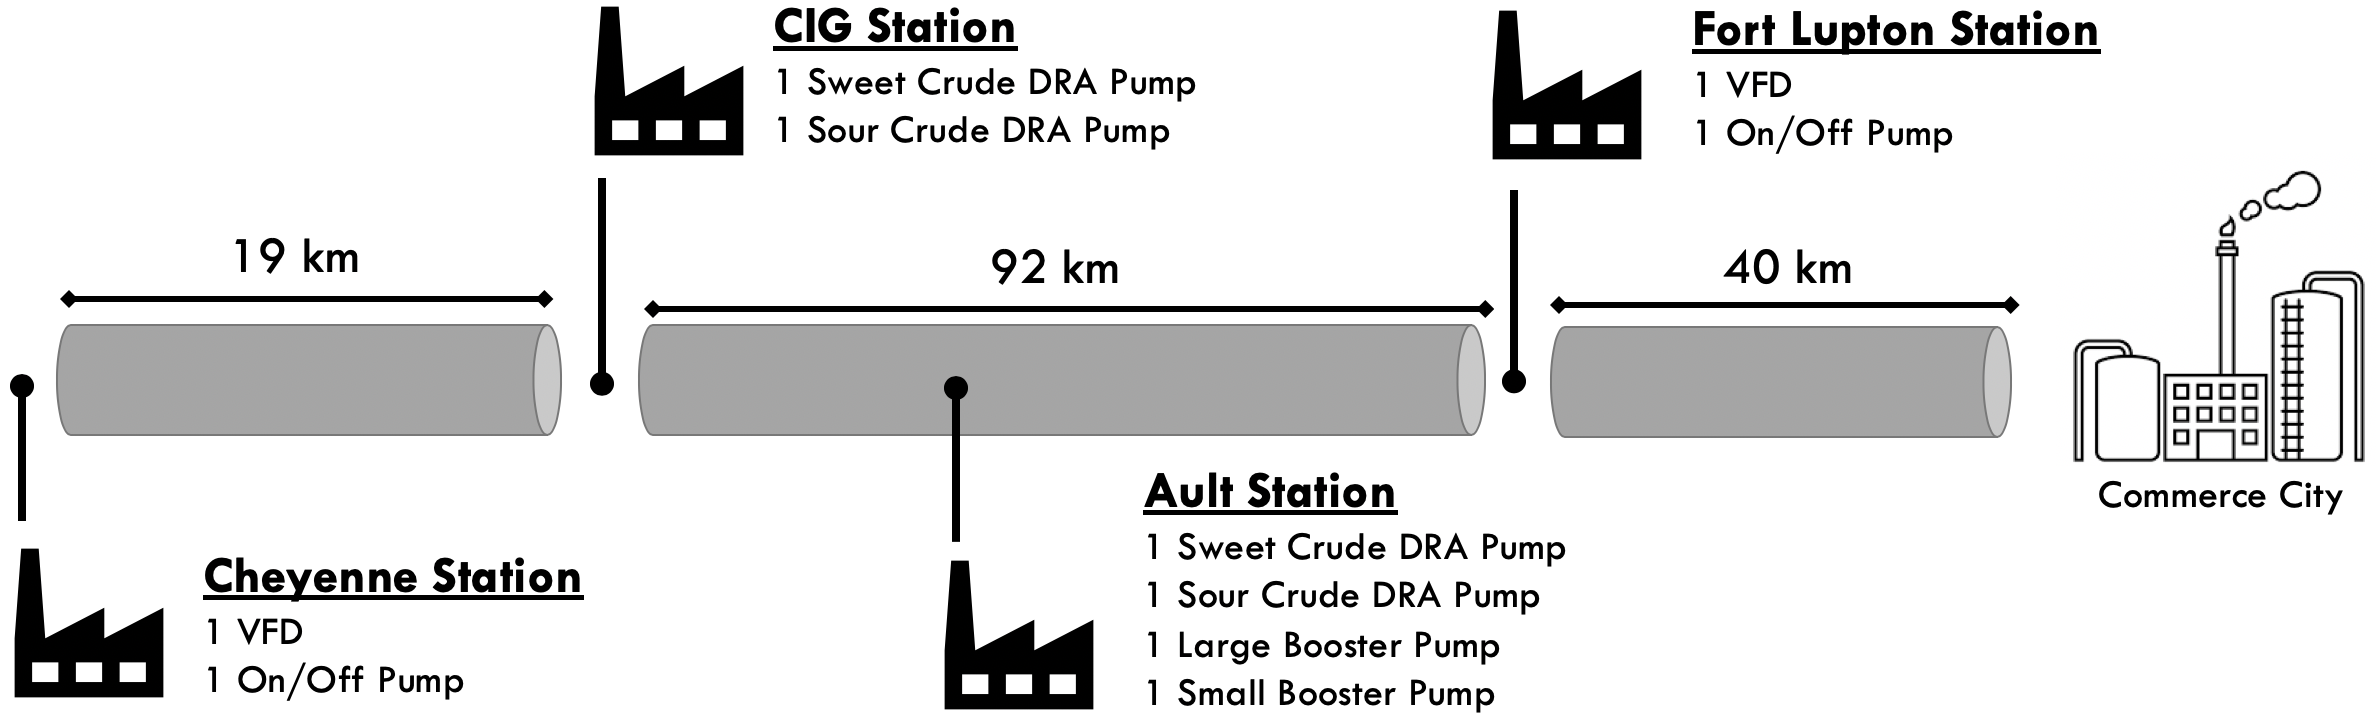
\includegraphics[scale=0.35]{images/08RM06A.png}
    \caption{Schematic diagram of Line RM06A.}
    \label{fig:08RM06A}
\end{figure}

Equipment wise, Line RM06A boasts eight pumps spread across four pump stations. Two pumps are variable frequency drives (VFD), while the rest are on/off pumps. Additionally, there are four drag reducing agent (DRA) injection pumps situated across the second and third pump stations. Each pump station contains a sour crude and sweet crude DRA pump. The sour and sweet crude uses different types of DRA.  The DRA is injected based on the product present at the pump station. 

\section{Anomaly Detection}
\subsection{Data Pre-processing}
\subsection{Data Set Creation}
\subsubsection{Generative Modelling}
\subsection{Model Identification}
\subsection{Conceptual Software Design}

\section{Real Time Optimization}
Modern control systems typically consists of three layers: real time optimization (RTO), supervisory control and regulatory control.  From the top, real time optimization is evaluated the least frequently, and performs a steady state optimization of the process.  The outputs of RTO are the ideal set points for all equipment given an operating objective.  Next, the supervisory control layer performs dynamic optimization to identify the most efficient input trajectory to achieve the set points from RTO. Supervisory control is evaluated faster than RTO, but slower than regulatory control. Model predictive control (MPC) and economic model predictive control (EMPC) are typical supervisory control frameworks. Finally, the regulatory controllers actuate physical equipment to achieve the input trajectory given by the supervisory control layer.  Common regulatory controllers are proportional-integral-derivative (PID) controllers.

The hierarchical structure of APC is shown in Figure \ref{fig:08APC}.

\begin{figure}[h]
    \centering
    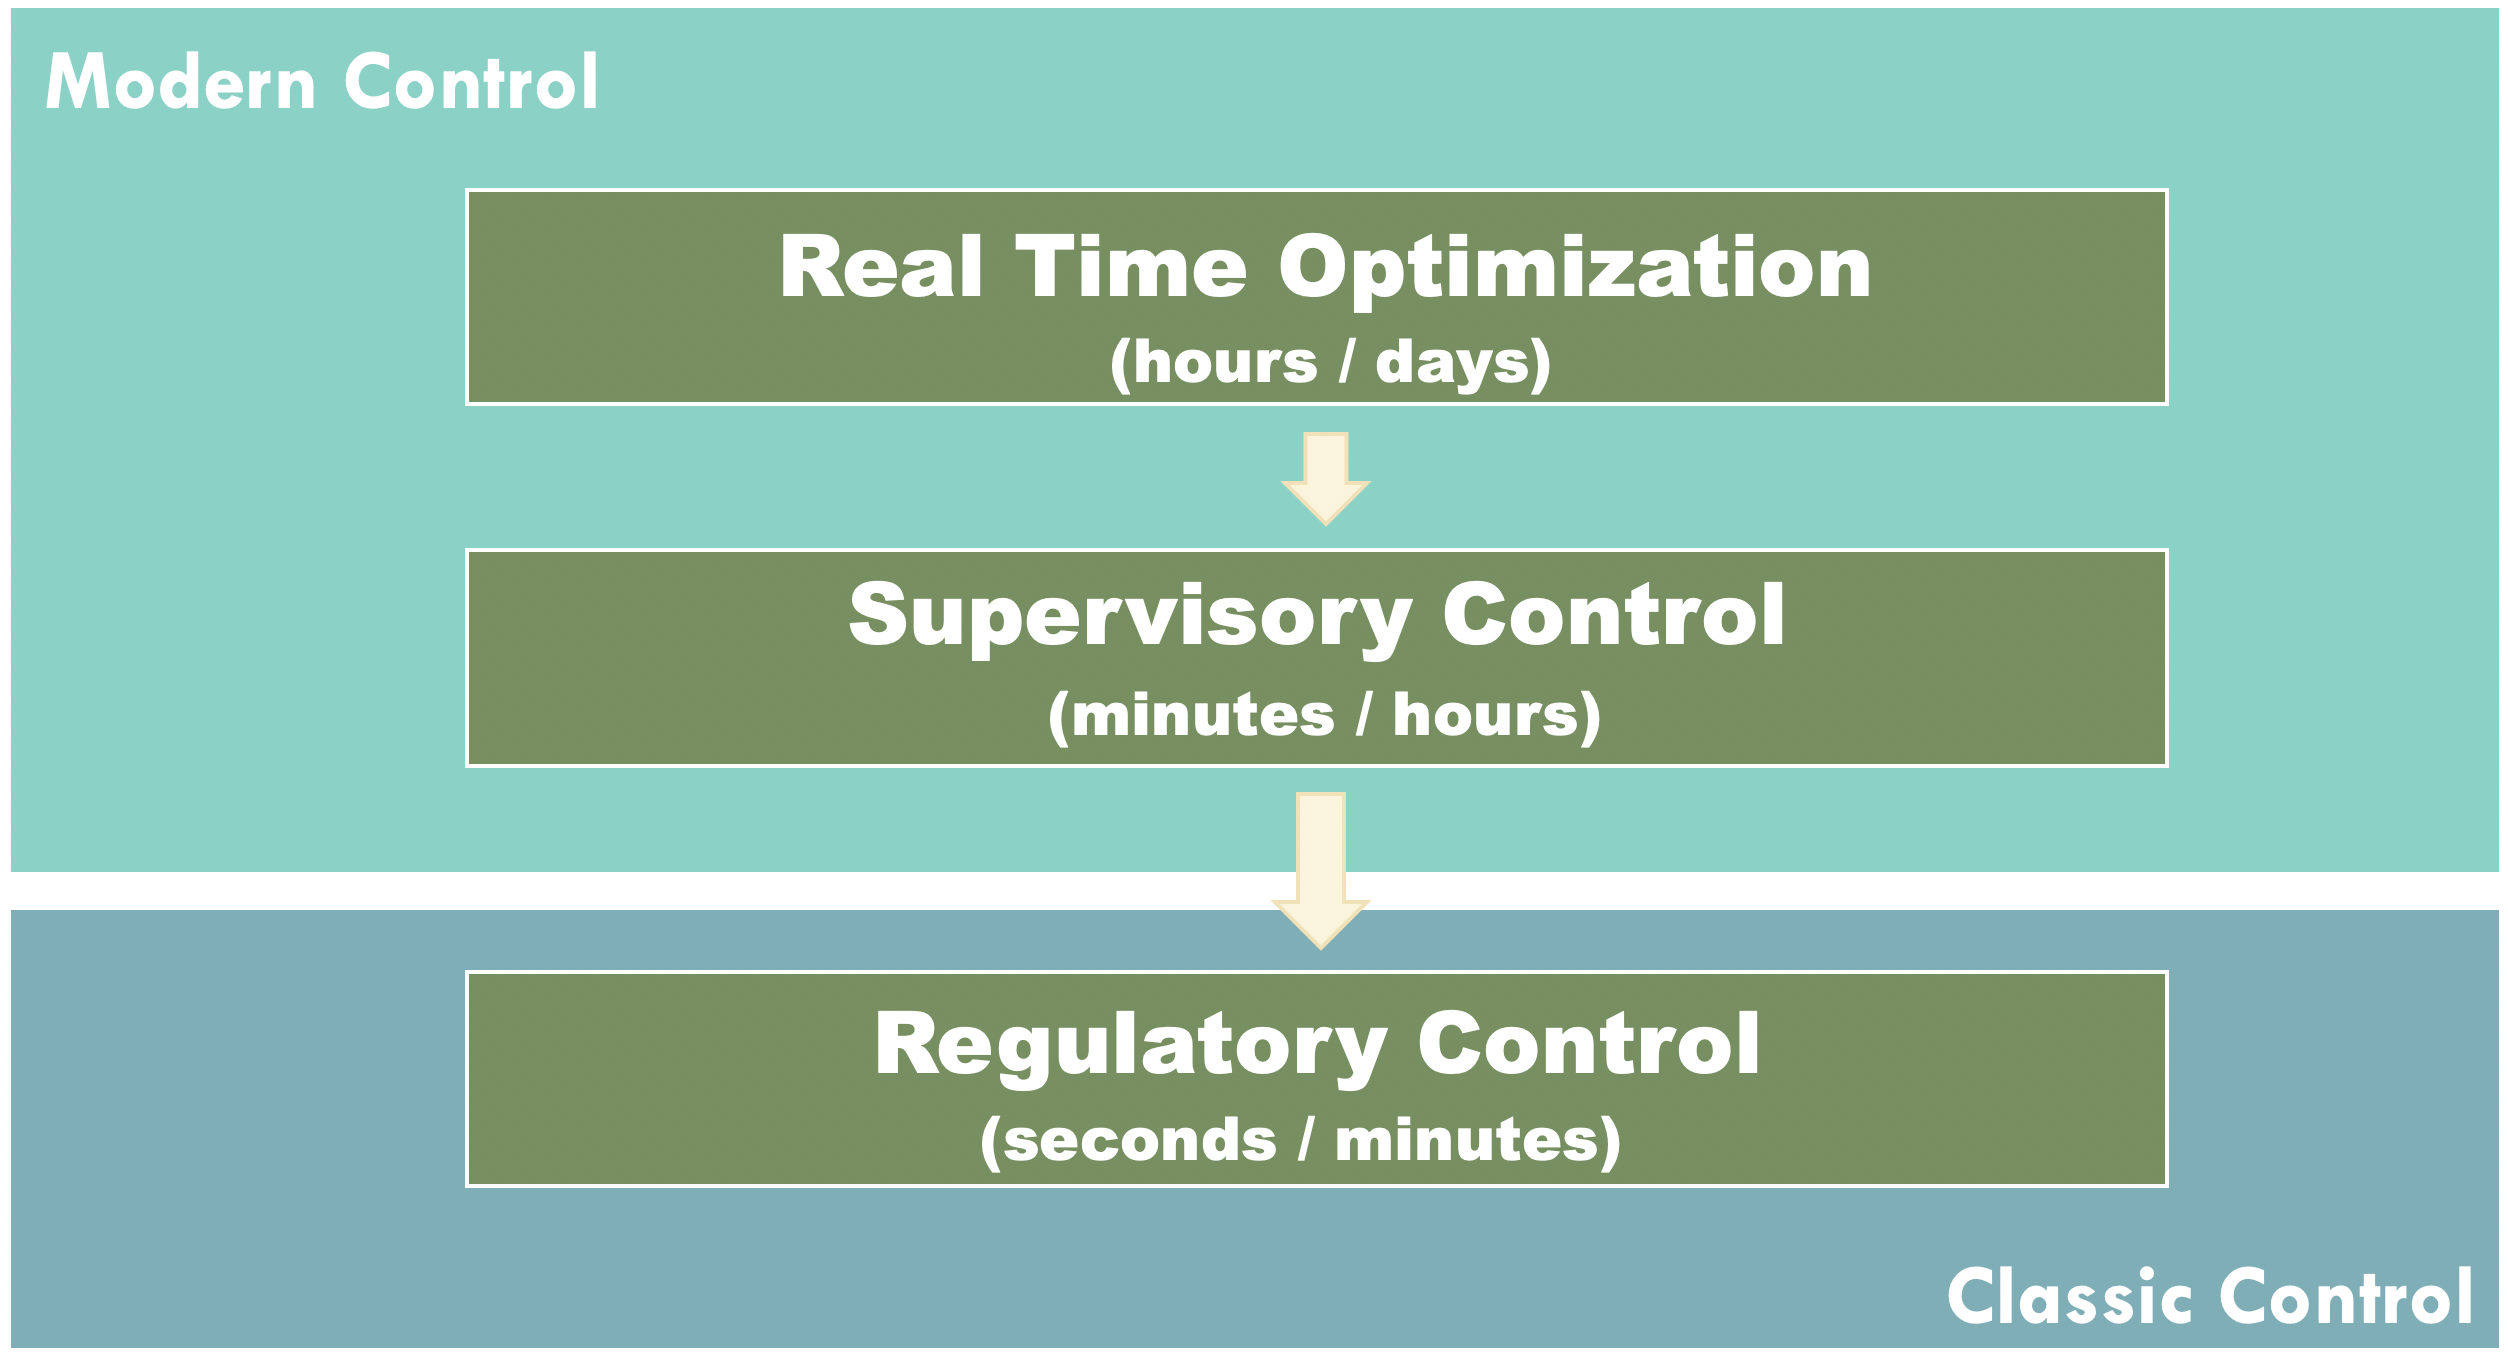
\includegraphics[scale=0.15]{images/08APC.png}
    \caption{Hierarchy of a typical control system.}
    \label{fig:08APC}
\end{figure}

\subsection{Problem Description}
Figure \ref{fig:08schedule} shows the communication framework of the pipeline operation. The goal of this pipeline is to meet the demands of the Commerce City refinery. To do so, a schedule with desired flow rates are sent to the operators from the scheduling team, and the operators are tasked to operate the pipeline at the given flow rate. Due to the complexity of this pipeline, different operators operate the pipeline differently depending on their own experience.  This difference introduces turbulence and unnecessary wear-and-tear onto the pipeline, increasing maintenance costs. Moreover, some operators are less experienced and operate the pipeline sub-optimally.

\begin{figure}[h]
    \centering
    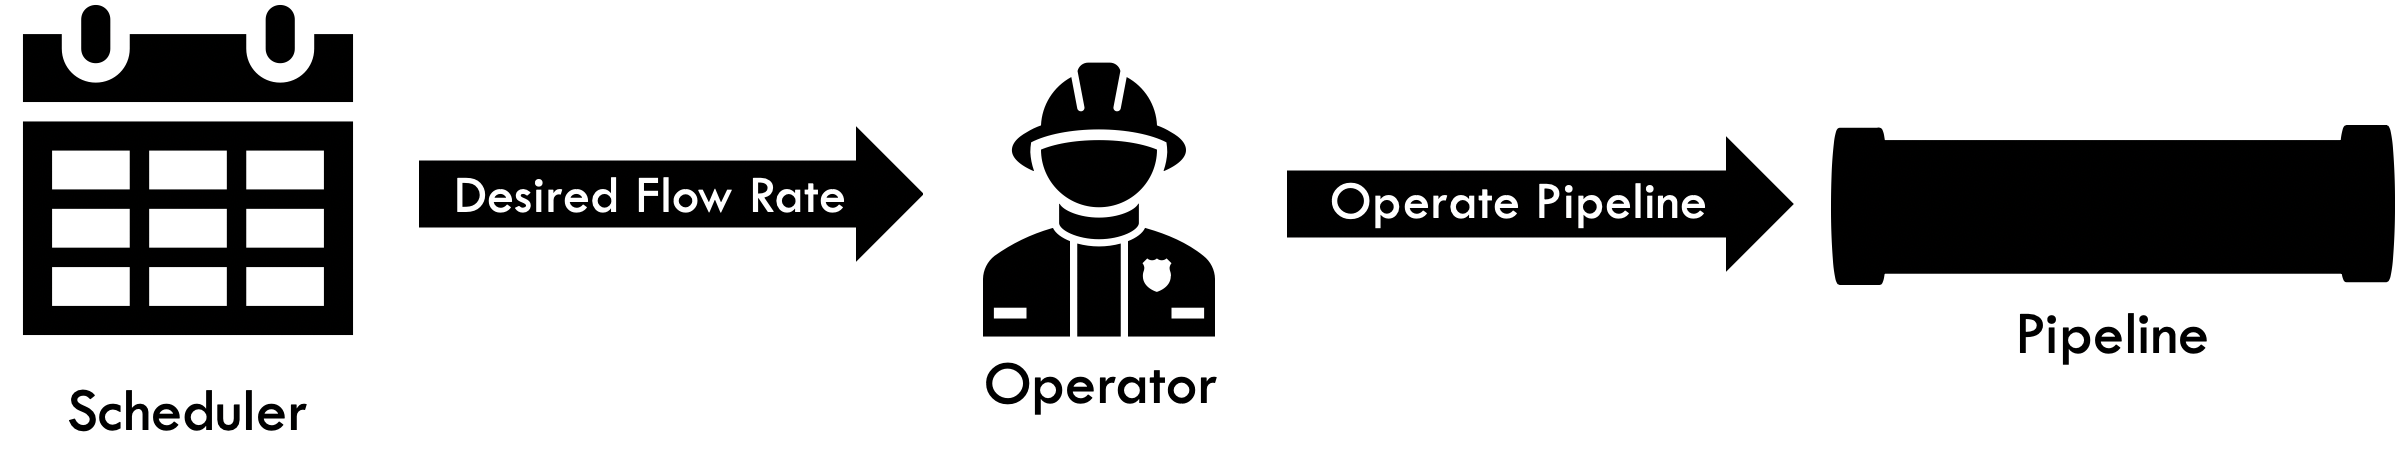
\includegraphics[scale=0.35]{images/08Schedule.png}
    \caption{Communication framework for operating line RM06A.}
    \label{fig:08schedule}
\end{figure}

To overcome this problem, machine learning was used to identify a model of the pipeline.  Then, a steady state optimization tool was built using mixed integer linear programming to give operators the \textbf{optimal} set-points for each equipment.  This system solves two problems: i) Introduces uniformity in operator behaviour for desired set-points. ii) Semi-automation of the pipeline, freeing up operators' time for other tasks.

The new communication framework for line RM06A is shown in Figure \ref{fig:08scheduleV2}.

\begin{figure}[h]
    \centering
    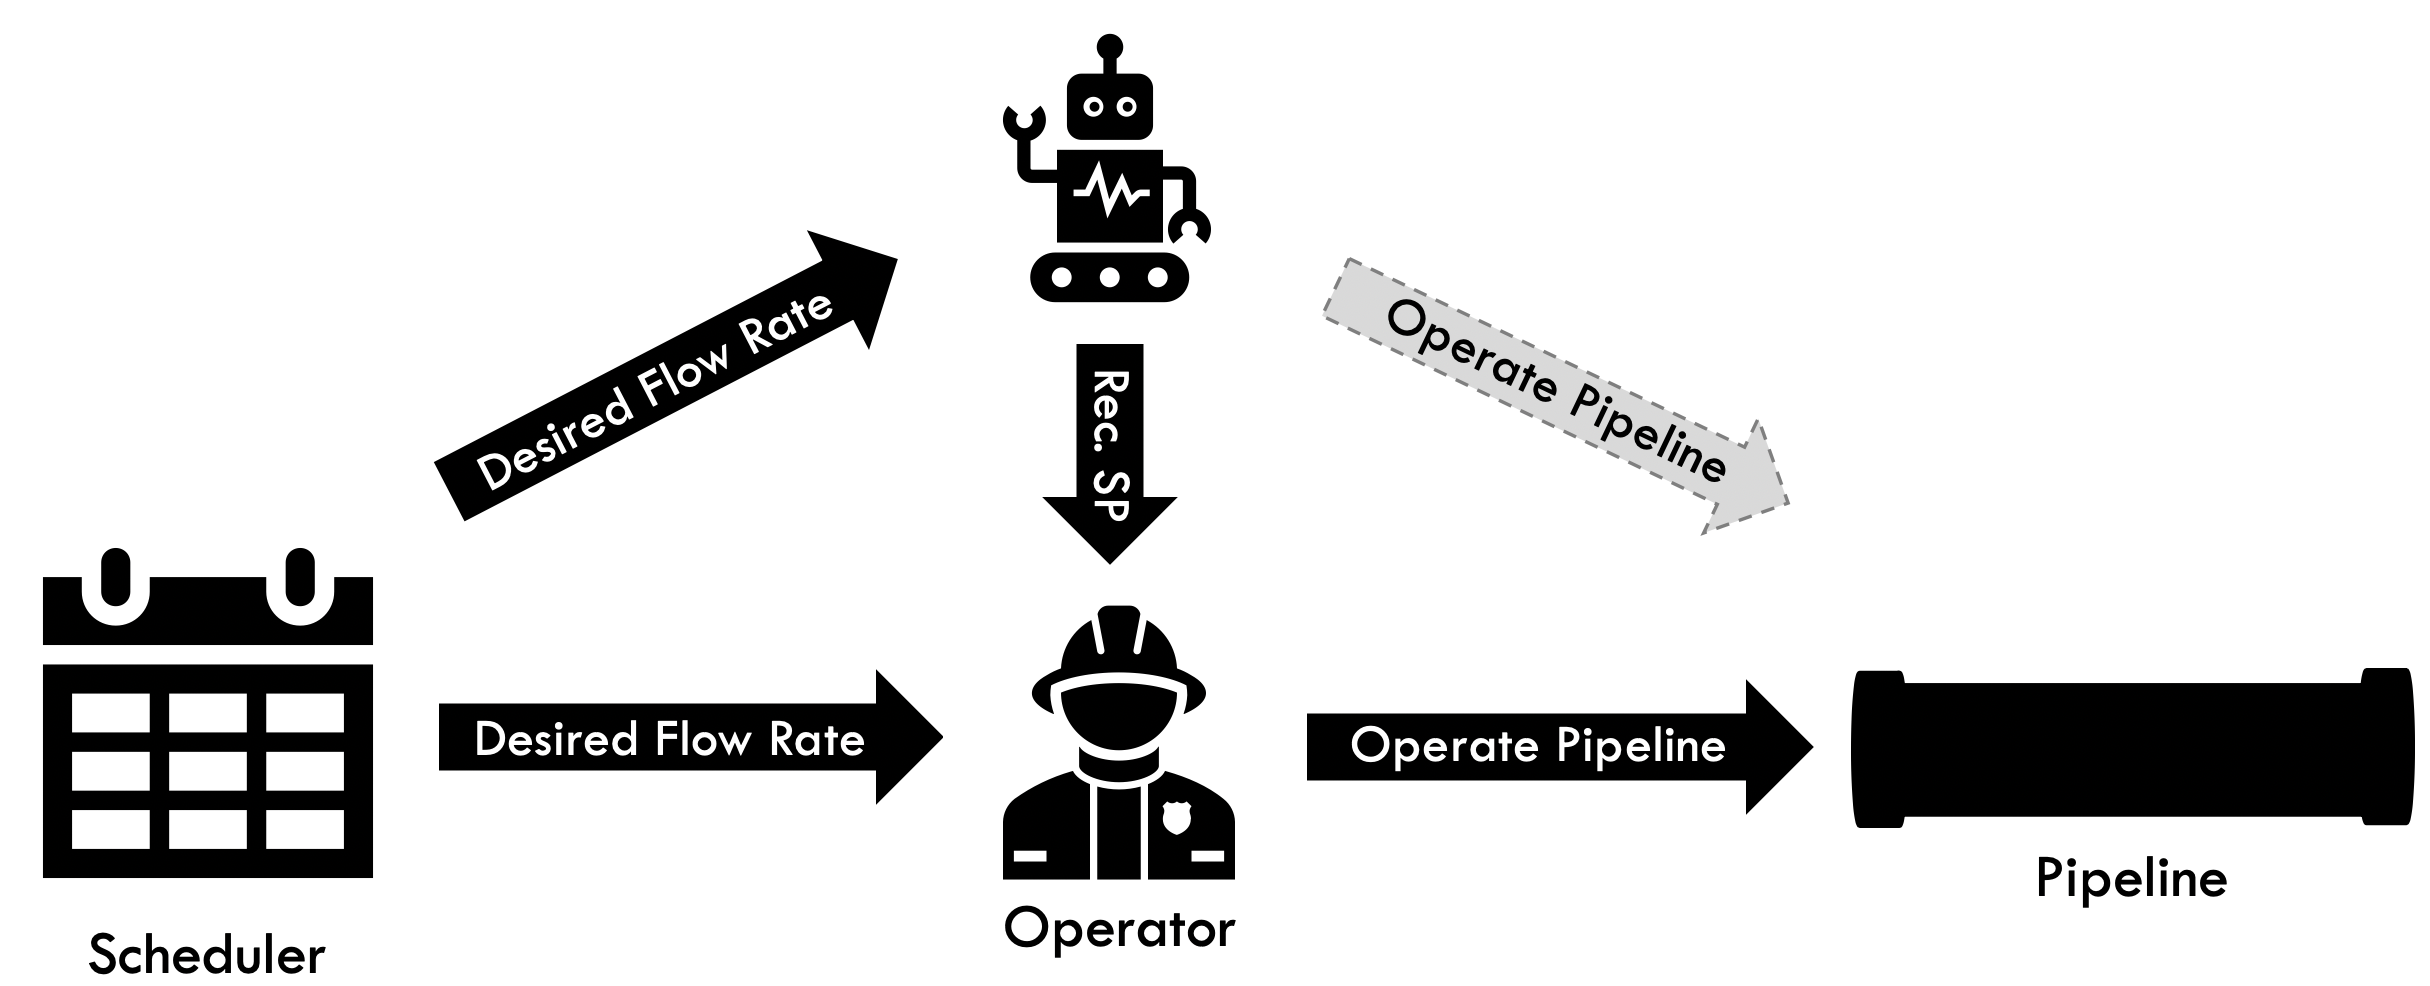
\includegraphics[scale=0.35]{images/08ScheduleV2.png}
    \caption{Proposed communication framework for operating line RM06A.}
    \label{fig:08scheduleV2}
\end{figure}

The rest of the section is organized as follows.  First, the data pre-processing step will be shown.  Then, the model identification phase will be introduced.  Following that, the optimization algorithm and all it's constraints for real-time optimization are presented.  Finally, the section is concluded with some conceptual software design regarding its implementation into a supervisory control and data acquisition (SCADA) system and the overall project impact will also be shown.

\subsection{Data Pre-processing}
Two data sets were initially provided by Suncor.  The details are shown in Table \ref{tab:08data}. Model identification and optimization evaluations were conducted for both datasets; however, the steps are very similar.  Because the 2019 algorithm will go into live production whereas the 2018 data was used primarily as a proof of concept, only the 2019 algorithm steps will be shown in detail.

\begin{table}[h]
    \centering
    {\setstretch{1.2}
    \begin{tabular}{ c | c }
        Date of Collection     &      Data Dimension      \\
        \hline
        June 2017 - June 2018  &    $525,601 \times 899$   \\
        Dec. 2018 - March 2019 &    $159,851 \times 738$   \\
    \end{tabular}}
    \caption{Suncor data details.}
    \label{tab:08data}
\end{table}

Data pre-processing can be broken down into three phases: Filtering by subject matter experts, automated data pre-processing, and manual data pre-processing.  An iterative procedure followed phase three where the subject matter experts worked alongside the machine learning scientists to give suggestions on which variables should be included/excluded in the final model.

\subsubsection{Filtering by Subject Matter Experts}
The first phase of data pre-processing was conducted by the subject matter experts at Suncor.  The original data set contained all data corresponding to the pipeline.  Variables such as alarm limits, fire detector status, monitor on/off status, etc., have low predictive power and were removed.  After this phase, the number of variables reduced from 738 to 124.  

The distribution of the remaining variables along the pipeline can be seen in Table \ref{tab:08Ph1Data}.

\begin{table}[h]
    \centering
    {\setstretch{1.2}
    \begin{tabular}{ c | c | c | c | c | c | c}
             &  Cheyenne & CIG & Ault & Fort Lupton & Comm. City & Other      \\
        \hline
        \# of Variables  &  24  &  21  &  21  &  33  &  22  &  3  \\
    \end{tabular}}
    \caption{Distribution of variables along line RM06A after phase 1 data pre-processing.}
    \label{tab:08Ph1Data}
\end{table}

\subsubsection{Automated Data Pre-processing}
Next, the data set was automatically filtered using the following methods:

\begin{itemize}
    \item \textbf{Missing data removal}: Remove \textit{rows} of data containing missing data.
    \item \textbf{Data imbalance analysis}: Remove boolean variables that contain 97\% or more of a single class.  Heavily imbalanced variables create model biases towards the majority class \cite{data_preprocessing}.
    \item \textbf{Collinear analysis}: Identify variables that are correlated over 90\%. Correlation, $r_{xy}$ is given in Equation \ref{eq:08correlation}. After corrlated variables are identified, one variable is kept while the rest are removed.  This is done to avoid redundant parameters \cite{data_preprocessing}.
    \begin{equation}
        r_{xy} = \frac{\sum(x_i - \bar{x})(y_i - \bar{y})}{\sqrt{\sum(x_i - \bar{x})^2\sum(y_i-\bar{y})^2}}
        \label{eq:08correlation}
    \end{equation}
    
\end{itemize}

After performing the above methods, the data set reduced from 124 to 65. The distribution of the new data set is shown in Table \ref{tab:08Ph2Data}.
\begin{table}[h]
    \centering
    {\setstretch{1.2}
    \begin{tabular}{ c | c | c | c | c | c | c}
             &  Cheyenne & CIG & Ault & Fort Lupton & Comm. City & Other      \\
        \hline
        \# of Variables  &  10  &  11  &  11  &  18  &  12  &  3  \\
    \end{tabular}}
    \caption{Distribution of variables along line RM06A after phase 2 data pre-processing.}
    \label{tab:08Ph2Data}
\end{table}

\subsubsection{Manual Data Pre-processing}
The data set is then manually pre-processed to remove or modify data from badly behaving sensors and irregular operating conditions.  In this phase, only the number of training examples are reduced.

For this pipeline, both sweet and sour crude are transported in a cyclical fashion due to the hydraulic dynamics of the pipeline. Otherwise, the sour crude is too heavy to be transported for sustainable periods. However, downstream demand for each product can disrupt this operating cycle.  From Figure \ref{fig:08API}, it can be seen that there were extended periods of time where only sweet or sour crude were being transported, and was caused by the lack of demand downstream.  Such scenarios deviate from normal operations and were removed from the data.

\begin{figure}[h]
     \centering
     \begin{subfigure}[b]{1.0\textwidth}
         \centering
         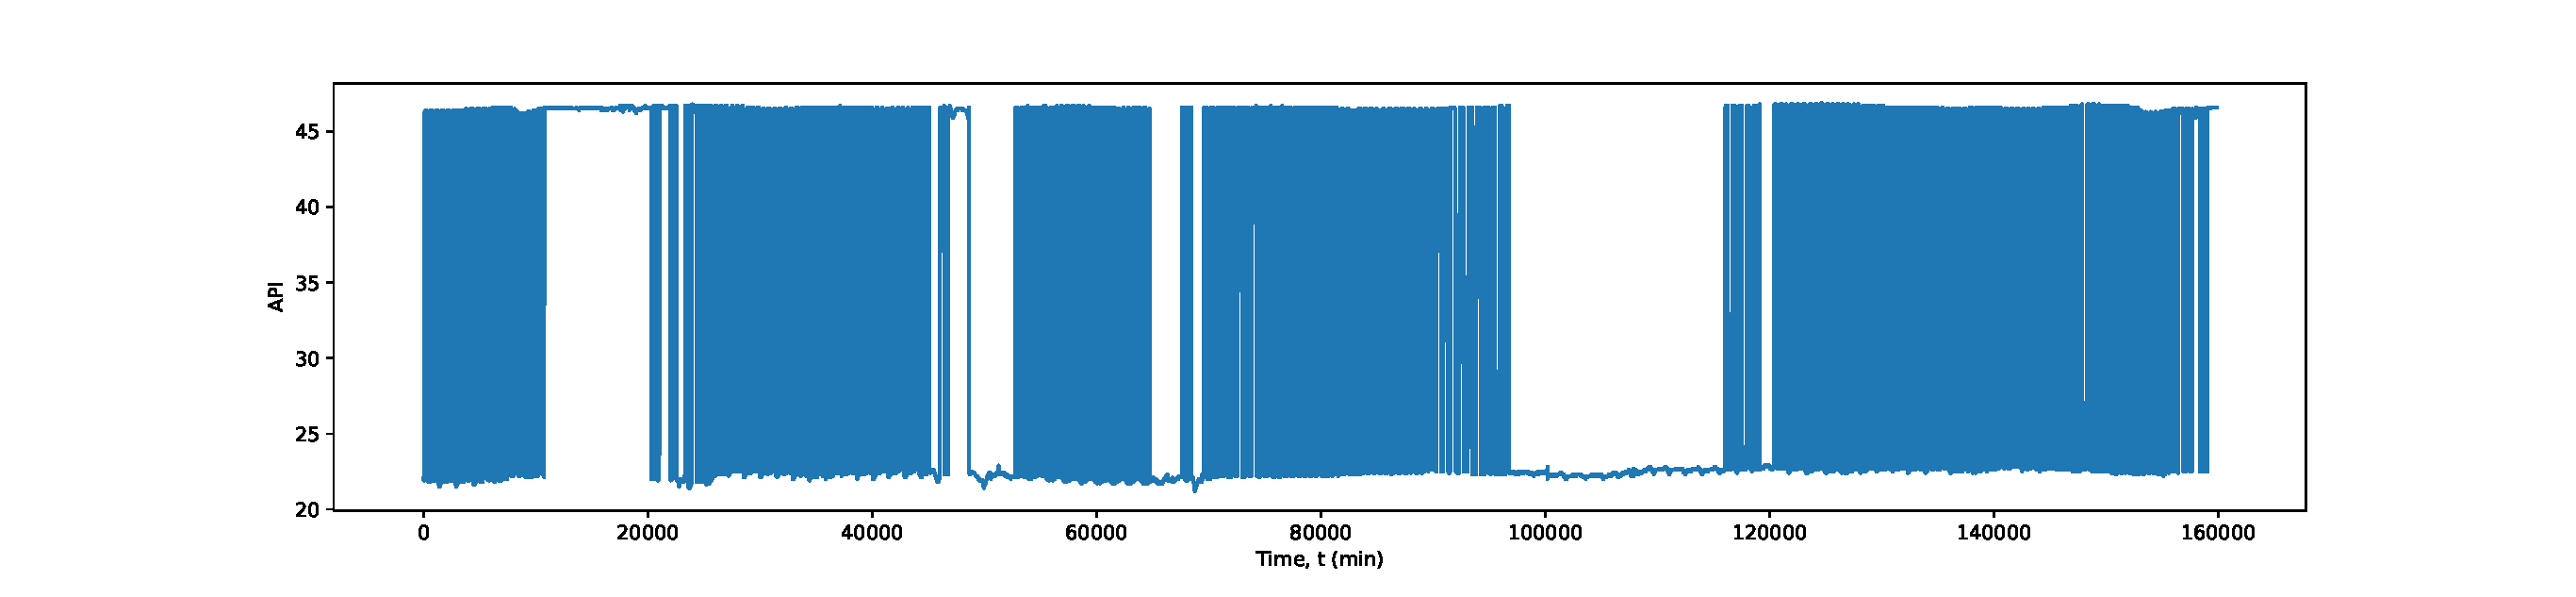
\includegraphics[width=\textwidth]{images/08NonFilteredDensity.eps}
         \caption{API data before abnormal condition removal.}
         \label{fig:08APIBefore}
     \end{subfigure}
     \hfill
     \begin{subfigure}[b]{1.0\textwidth}
         \centering
         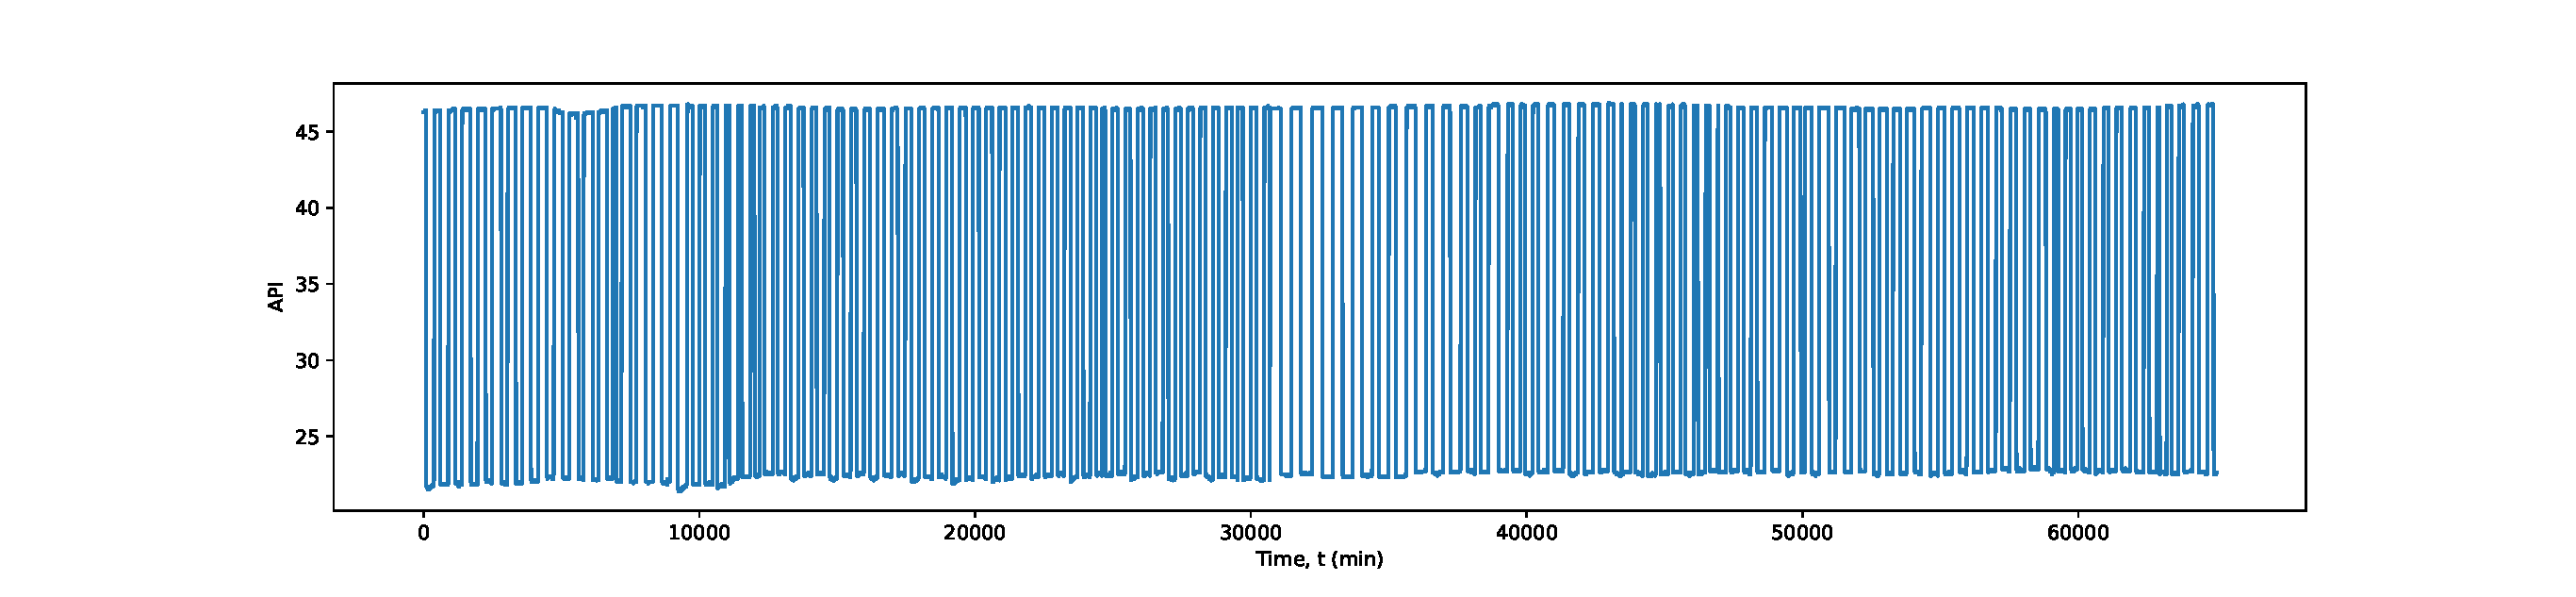
\includegraphics[width=\textwidth]{images/08FilteredDensity.eps}
         \caption{API data after abnormal condition removal.}
         \label{fig:08APIAfter}
     \end{subfigure}
        \caption{API data before and after removing abnormal operating conditions.}
        \label{fig:08API}
\end{figure}

Moreover, there is a time delay for the flow rate to react to a DRA set point change because the new DRA concentration must be transported throughout the line before its effect can be fully realized.  DRA is assumed to be catastrophically destroyed when passing through a pump; thus, DRA is only required to coat the pipeline between pump stations for its full effect to be exploited.  For CIG, it must coat the pipeline between CIG to Ault.  For Ault, the pipeline spanning between Ault and Fort Lupton must be coated.  Given the flow rate of the pipeline, it will take approximately ten hours to sufficiently coat the majority of the pipeline. Hence, data corresponding to transitional periods are removed. At times, transitional times may take longer; however, removing additional data will reduce the available data for model identification.  

Pre- and post-processed DRA parts per million (ppm) measurements are shown in Figure \ref{fig:08DRA}. DRA ppm is measured continuously for the control of the DRA injection pumps. However, the measurement is unreliable and corrupted with noise. Because DRA set points are rarely changed, an exponentially weighted moving average (EWMA) was applied to the DRA ppm readings for increased measurement reliability.  The EWMA formula and bias correction are given in Equations \ref{eq:08EWMA} and \ref{eq:08Bias_Correction}, respectively: 
\begin{equation}
    v_t = \beta v_{t - 1} + (1 - \beta) \theta_t, \; v_0 = 0
    \label{eq:08EWMA}
\end{equation}
\begin{equation}
    v_t \leftarrow \frac{v_t}{1 - \beta^t}, \forall v \in V
    \label{eq:08Bias_Correction}
\end{equation}
where $v_{t}$ is the exponentially weighted value at time $t$.  $\beta$ is the exponentially weighing factor.  Larger $\beta$ results in smoother results.  $\theta_t$ is the original value at time $t$. $V$ is a vector representing the exponentially weighted values before bias correction.

The objective of the machine learning model was to predict the flow rate at Commerce City.  However, there is a natural time delay between the time an equipment status changed and the corresponding impact on downstream flow rate.  Because the pipeline is fully loaded and the product is incompressible, pressure changes upstream will be propagated downstream at close to the speed of sound \cite{fluid_mechanics}.  Table \ref{tab:08TimeToCC} shows the time required for pressure to propagate down the pipeline starting from each pump station.  The pump data for each pump station was shifted accordingly to account for this time delay.  
\begin{table}[h]
    \centering
    {\setstretch{1.2}
    \begin{tabular}{ p{6cm} | c | c | c | c}
             &  Cheyenne & CIG & Ault & Fort Lupton \\
        \hline
        Time to Commerce City at speed of sound in liquids (1480 m/s) \cite{fluid_mechanics}
        &  1.7 min  &  1.5 min  &  1.0 min  &  0.45 min  \\
    \end{tabular}}
    \caption{Time required for pressure changes at each pump station to be realized at Commerce City.}
    \label{tab:08TimeToCC}
\end{table}
\begin{figure}
     \centering
     \begin{subfigure}[b]{0.9\textwidth}
         \centering
         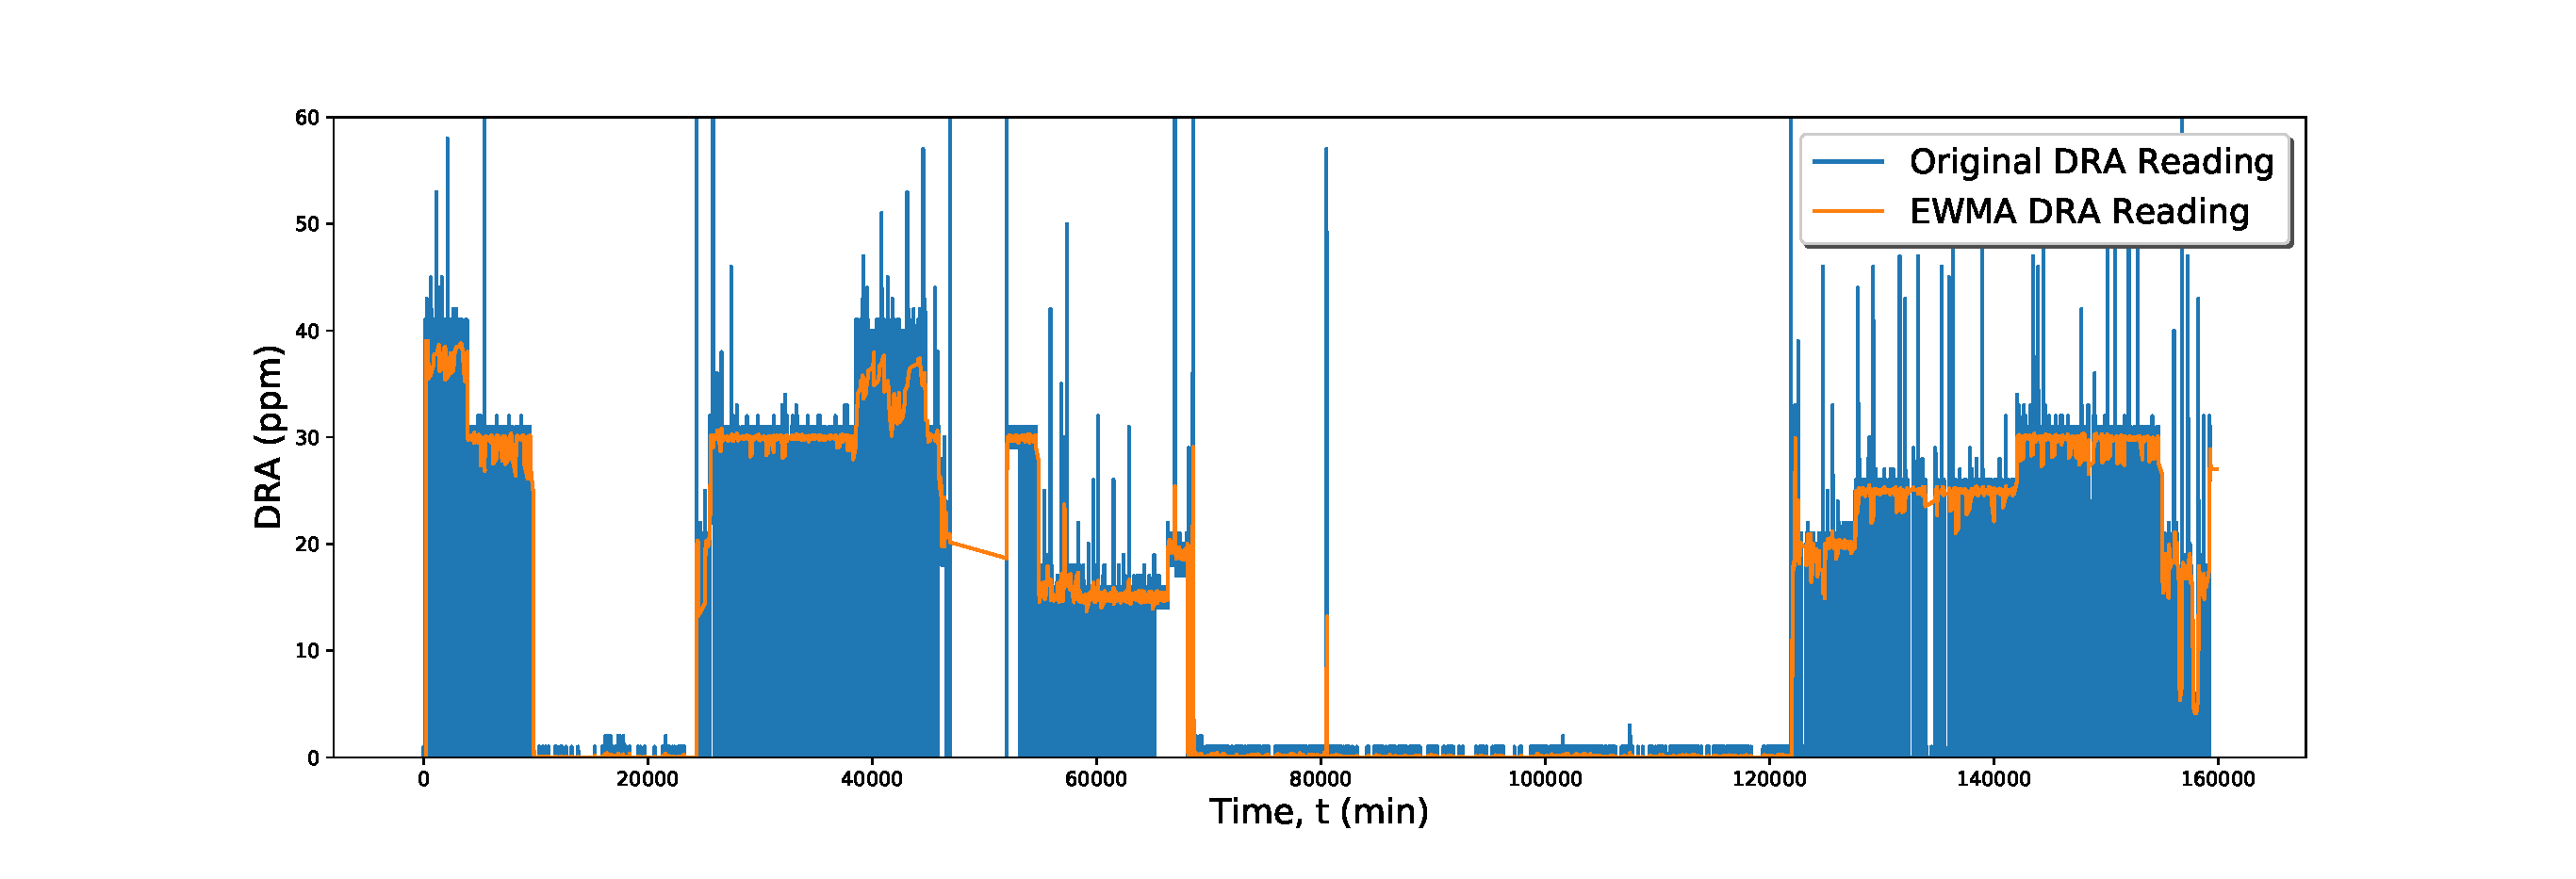
\includegraphics[width=\textwidth]{images/08CIGSour.eps}
         \caption{CIG sour DRA sensor reading.}
         \label{fig:08CIGSour}
     \end{subfigure}
     \begin{subfigure}[b]{0.9\textwidth}
         \centering
         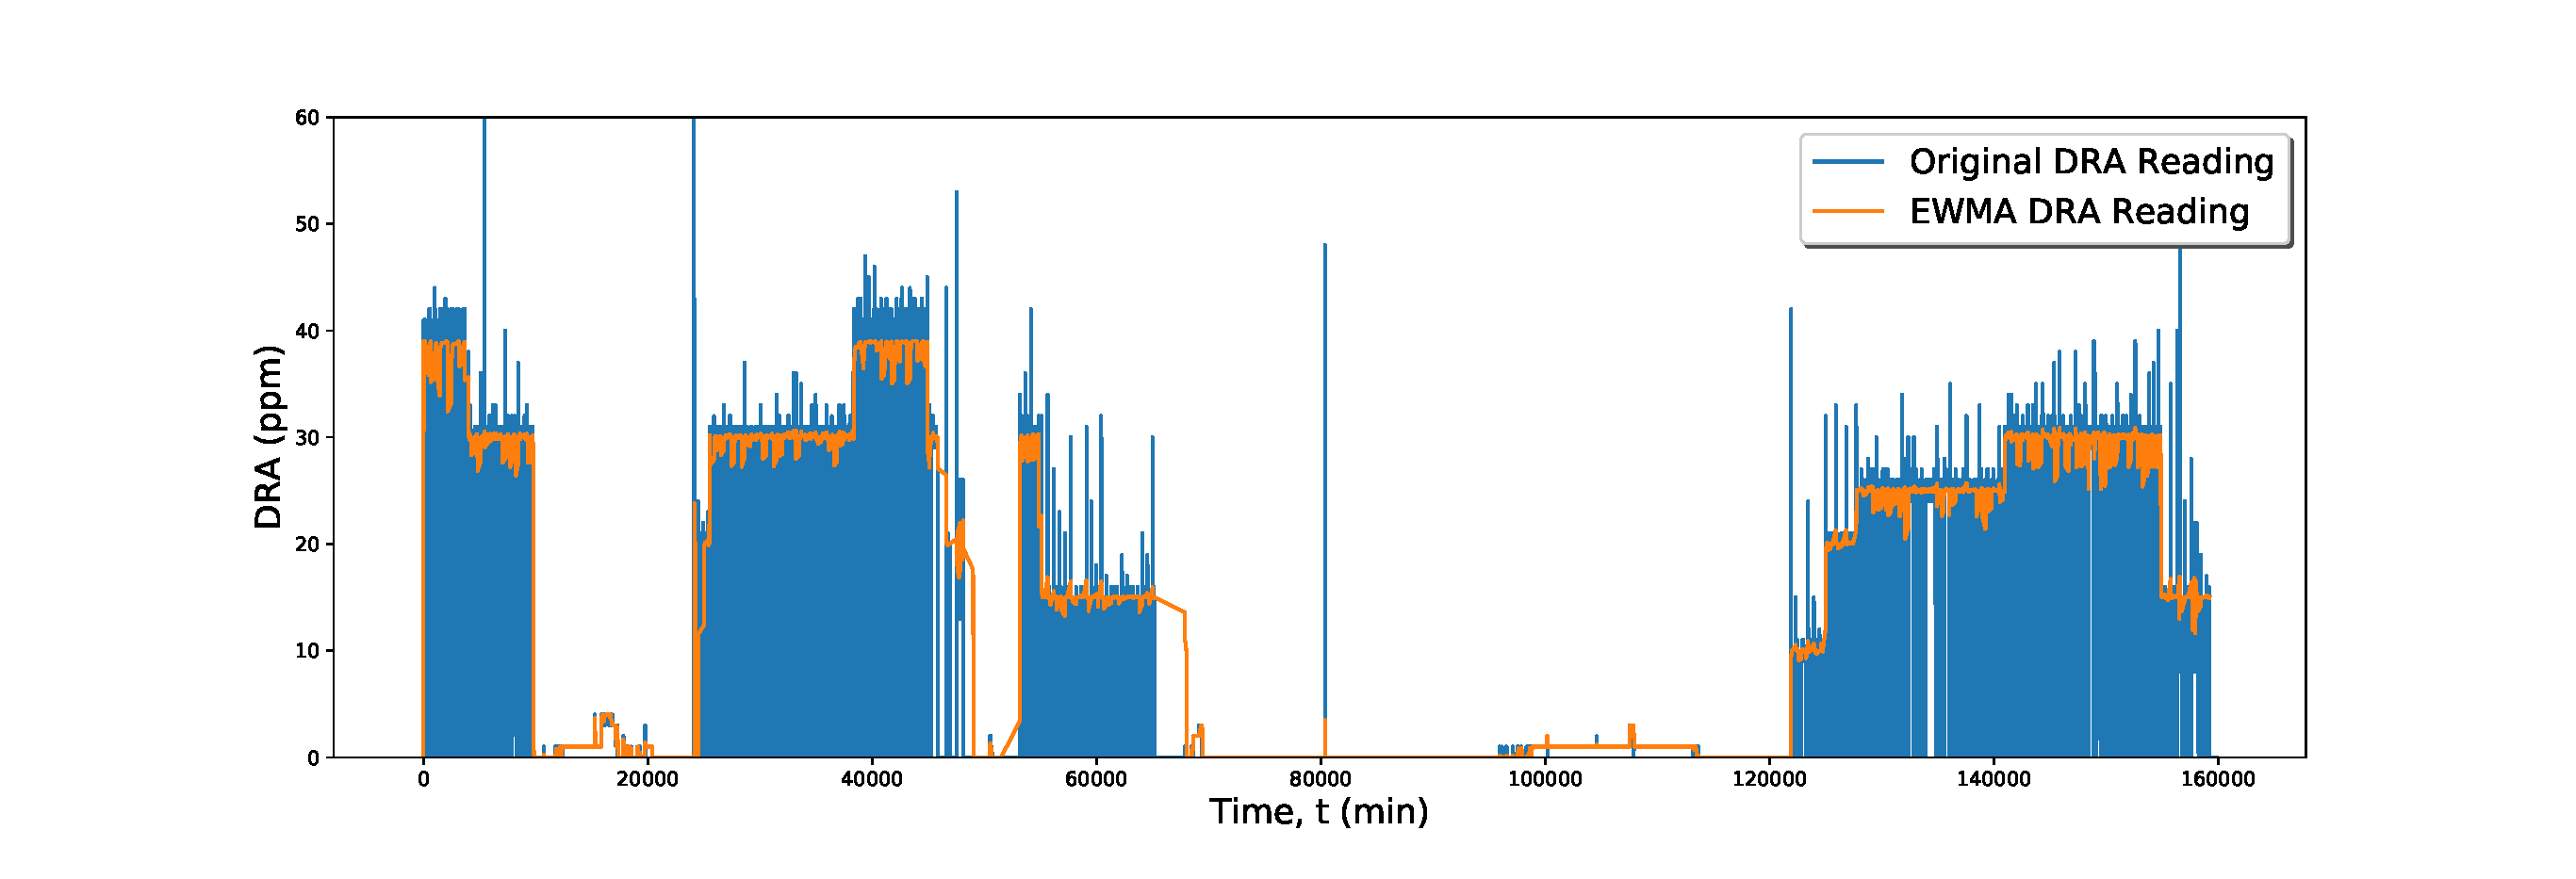
\includegraphics[width=\textwidth]{images/08CIGSweet.eps}
         \caption{CIG sweet DRA sensor reading.}
         \label{fig:08CIGSweet}
     \end{subfigure}
     \begin{subfigure}[b]{0.9\textwidth}
         \centering
         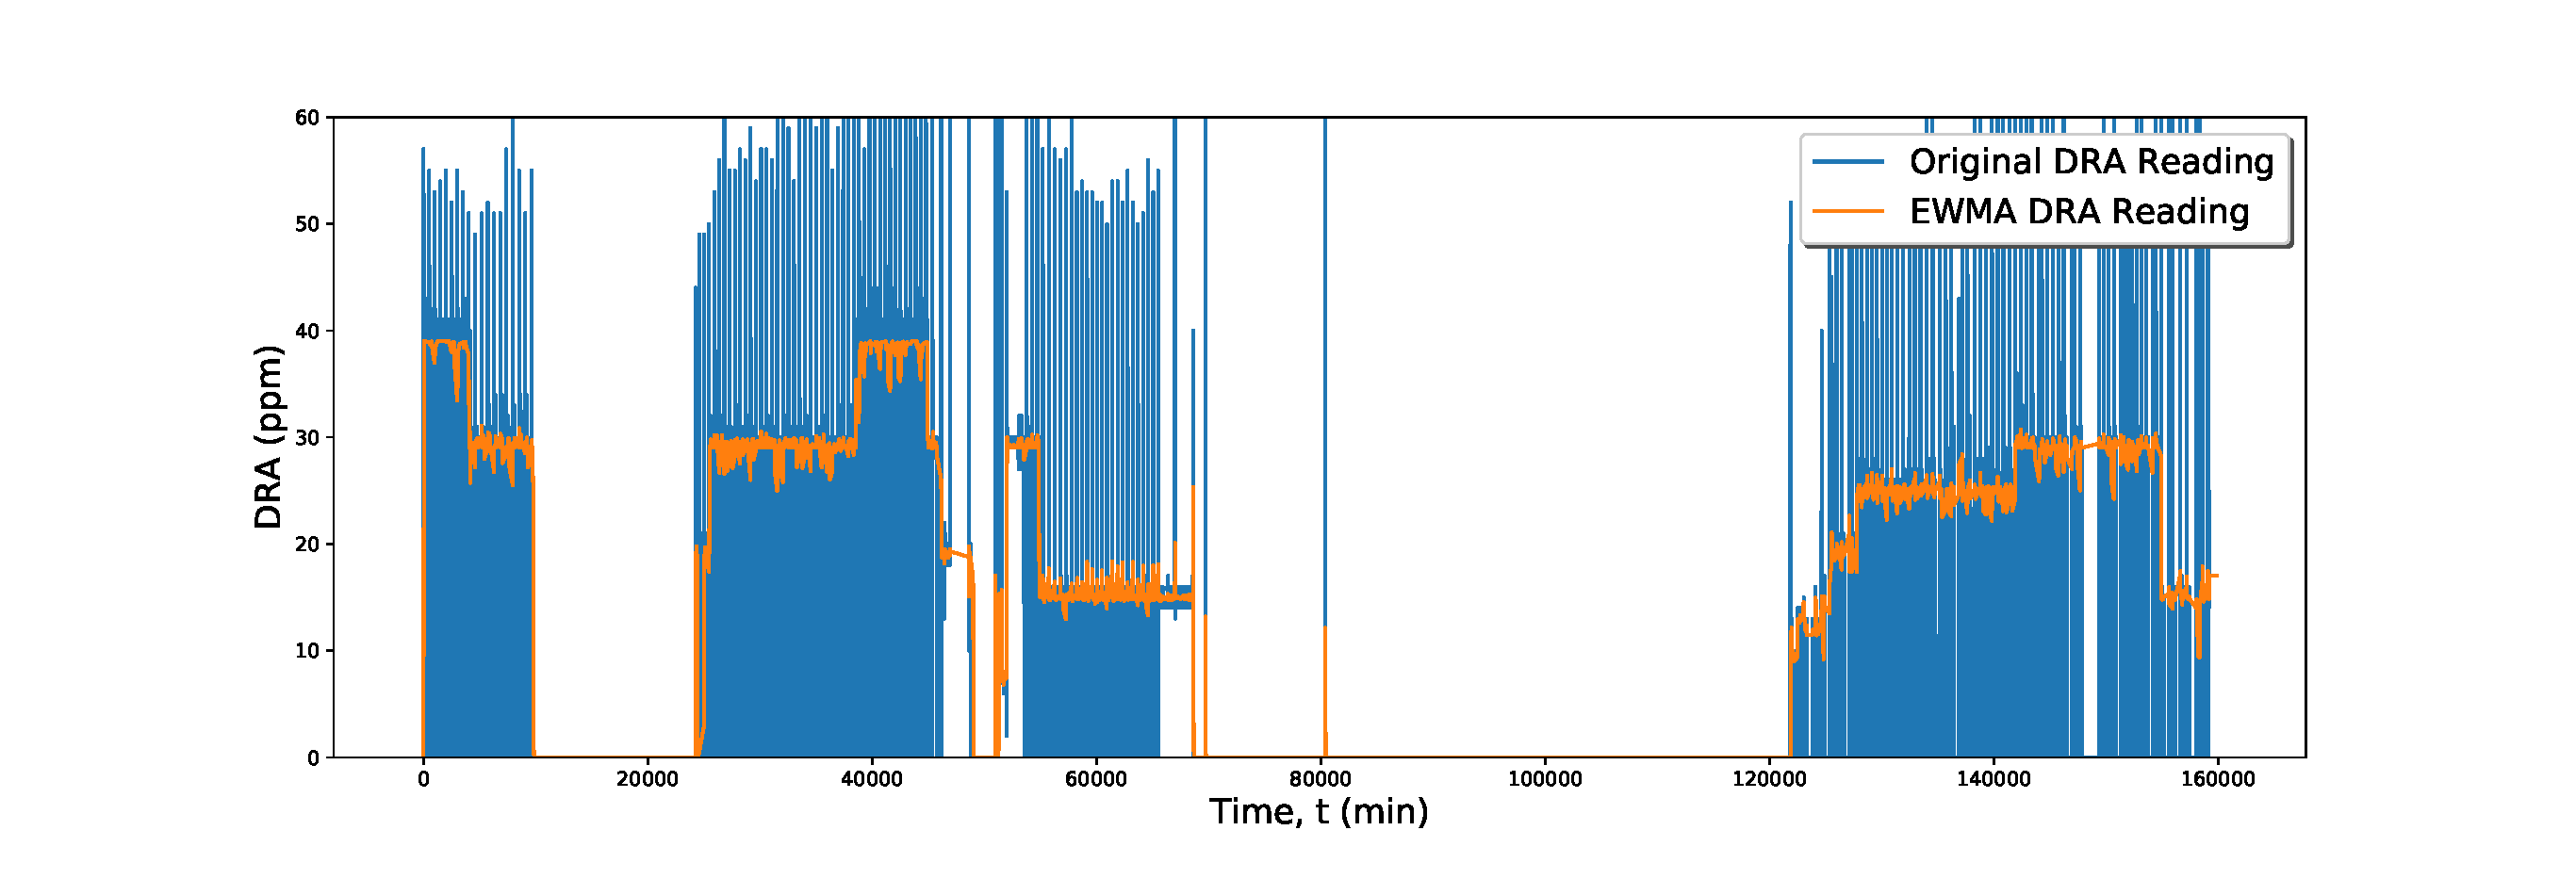
\includegraphics[width=\textwidth]{images/08AultSour.eps}
         \caption{Ault sour DRA sensor reading.}
         \label{fig:08AultSour}
     \end{subfigure}
     \begin{subfigure}[b]{0.9\textwidth}
         \centering
         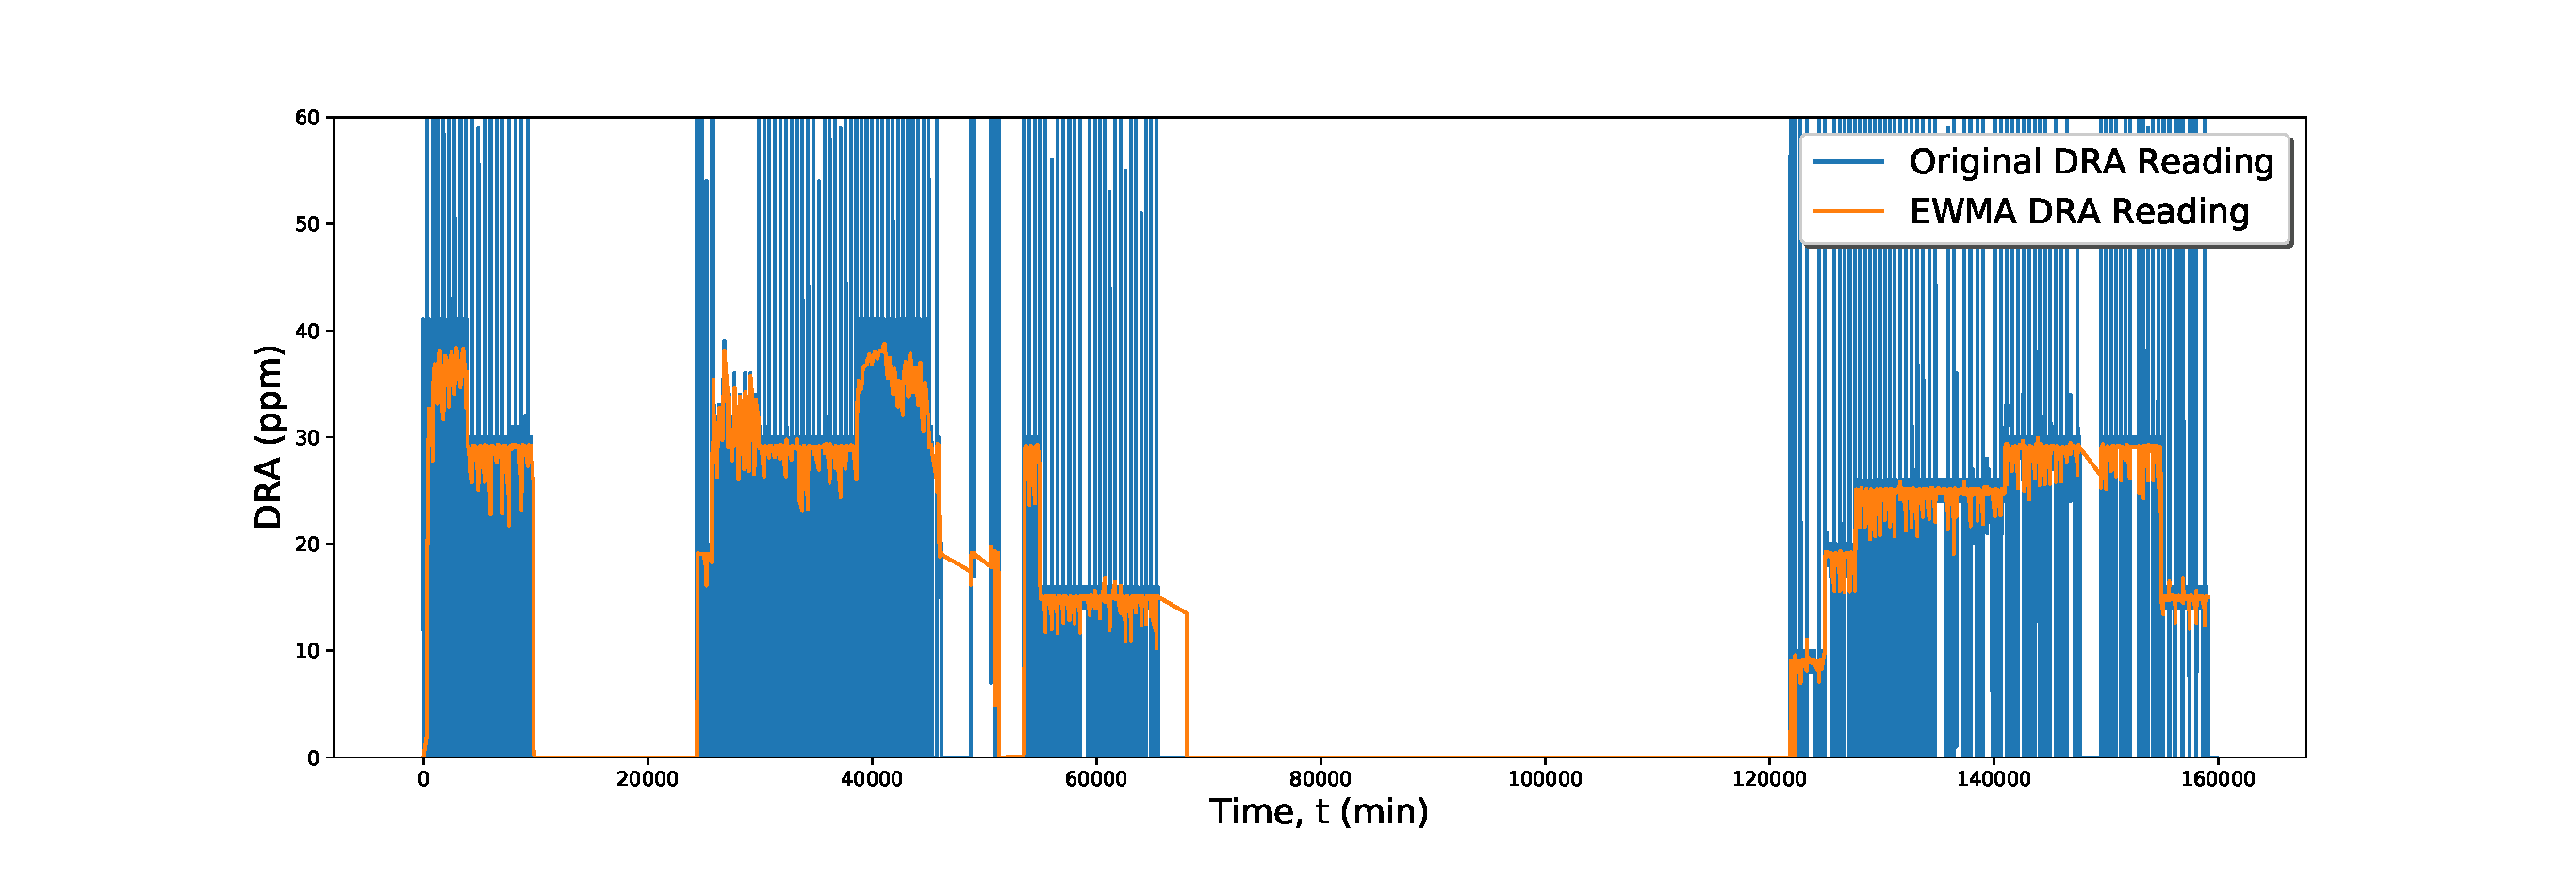
\includegraphics[width=\textwidth]{images/08AultSweet.eps}
         \caption{CIG sweet DRA sensor reading.}
         \label{fig:08AultSweet}
     \end{subfigure}
        \caption{Pre- and post-processed DRA sensor readings.}
        \label{fig:08DRA}
\end{figure}

A comprehensive list of the manual data pre-processing procedures is as follows:
\begin{enumerate}
    \item Shift data to accommodate the time delay at Commerce City.
    \item Smooth DRA data using exponentially weighted moving average given in Equation \ref{eq:08EWMA}.  
    \item Remove first 10 hours data corresponding to DRA set point changes.
    \item Remove data points where flow is under 800 bbl/hr.
    \item Remove data when only sweet or sour crude was sent through the pipeline.
\end{enumerate}

The final data set contained 65 variables and 97,470 data points.

\subsection{Model Identification}
\subsubsection{Feature Selection}
For each pump station, there was a variety of sensors measuring the same process variables.  For example, VFD pumps have four readings each: On/off status, RPM, HZ, and current. Many variables relating to one equipment is redundant; thus, only one variable was selected when redundancy existed. Additionally, some sensors were behaving abnormally.

In normal operations, the density fluctuates between 10 - 50 API, depending on the type of crude present in the pipeline.  After analysis, the Fort Lupton densitometer was behaving abnormally compared to other densitometer and is shown in Figure \ref{fig:08Density}.  After confirming with Suncor that the densitometer was behaving abnormally, the variable was removed.  
\begin{figure}[h]
     \centering
     \begin{subfigure}[b]{0.48\textwidth}
         \centering
         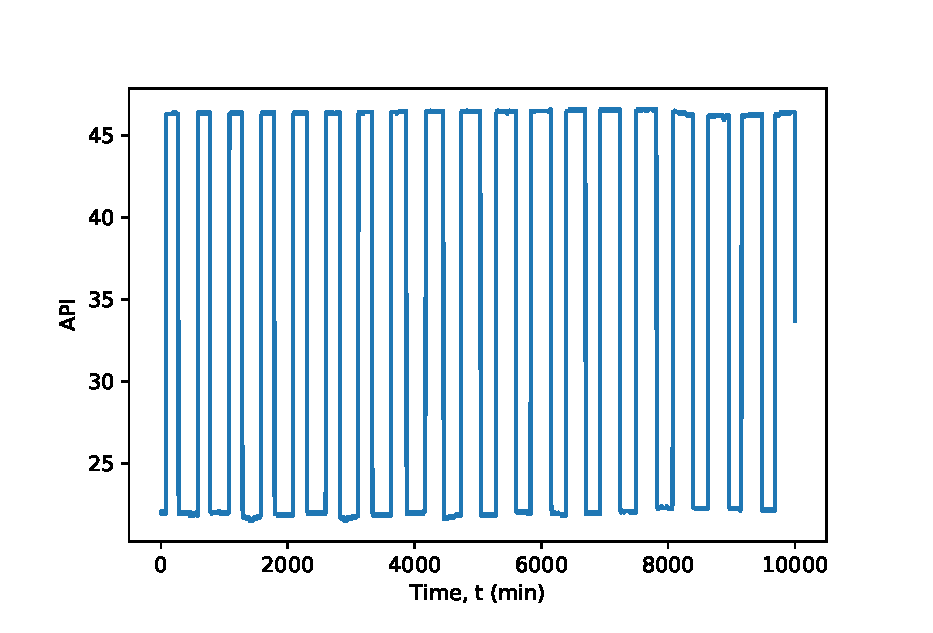
\includegraphics[width=\textwidth]{images/08CheyDensity.eps}
         \caption{Cheyenne API data for 10,000 mins.}
         \label{fig:08GoodDensity}
     \end{subfigure}
     \hfill
     \begin{subfigure}[b]{0.48\textwidth}
         \centering
         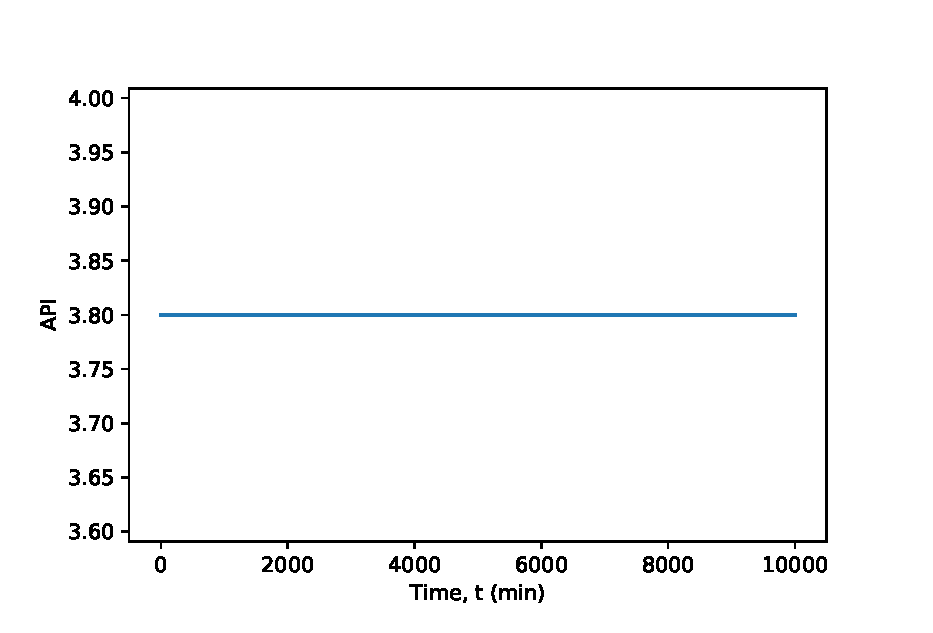
\includegraphics[width=\textwidth]{images/08FLDensity.eps}
         \caption{Fort Lupton API data for 10,000 mins.}
         \label{fig:08BadDensity}
     \end{subfigure}
        \caption{Comparison of normal and abnormal density readings.}
        \label{fig:08Density}
\end{figure}

Table \ref{tab:08featselect} shows the features selected for each pump station. The predicted variable was the flow rate (bbl/h) at Commerce City.
\begin{table}[h]
    \centering
    {\tiny
    {\setstretch{1.2}
    \begin{tabular}{ c | c | c | c | c}
        Cheyenne                       & CIG                      & Ault                        & Fort Lupton                    & Commerce City \\
        \hline
        $x_5$: Boos. Pump Status       &  $x_1$: Sweet DRA (ppm)  &  $x_3$: Sweet DRA (ppm)     &  $x_{8}$: Boos. Pump Status   &  $x_{18}$: Inlet Temp. (°C) \\
        
        $x_9$: VFD Current (Amp)       &  $x_2$: Sour DRA (ppm)   &  $x_4$: Sour DRA (ppm)      & $x_{10}$: VFD Current (Amp)      & \\
        
        $x_{14}$: Inlet Temp. (°C)     &  $x_{15}$: Inlet Temp. (°C) &  $x_6$: Small Pump Status &  $x_{17}$: Inlet Temp. (°C)  & \\
        
        $x_{11}$: API                   &  $x_{12}$: API          &  $x_7$: Large Pump Status   &             
        & \\
        
                                       &                          &  $x_{16}$: Inlet Temp. (°C)  &             
        & \\
        
                                       &                          &  $x_{13}$: API               &       
        & \\
        
    \end{tabular}}}
    \caption{Features selected for machine learning models.}
    \label{tab:08featselect}
\end{table}

\subsubsection{Feature Scaling}
Figure \ref{fig:08featscale} shows the contour of a normalized and non-normalized cost function. It can be seen that the optimization of a non-normalized cost function can be significantly hindered depending on where the optimization is initialized.

\begin{figure}[h]
    \centering
    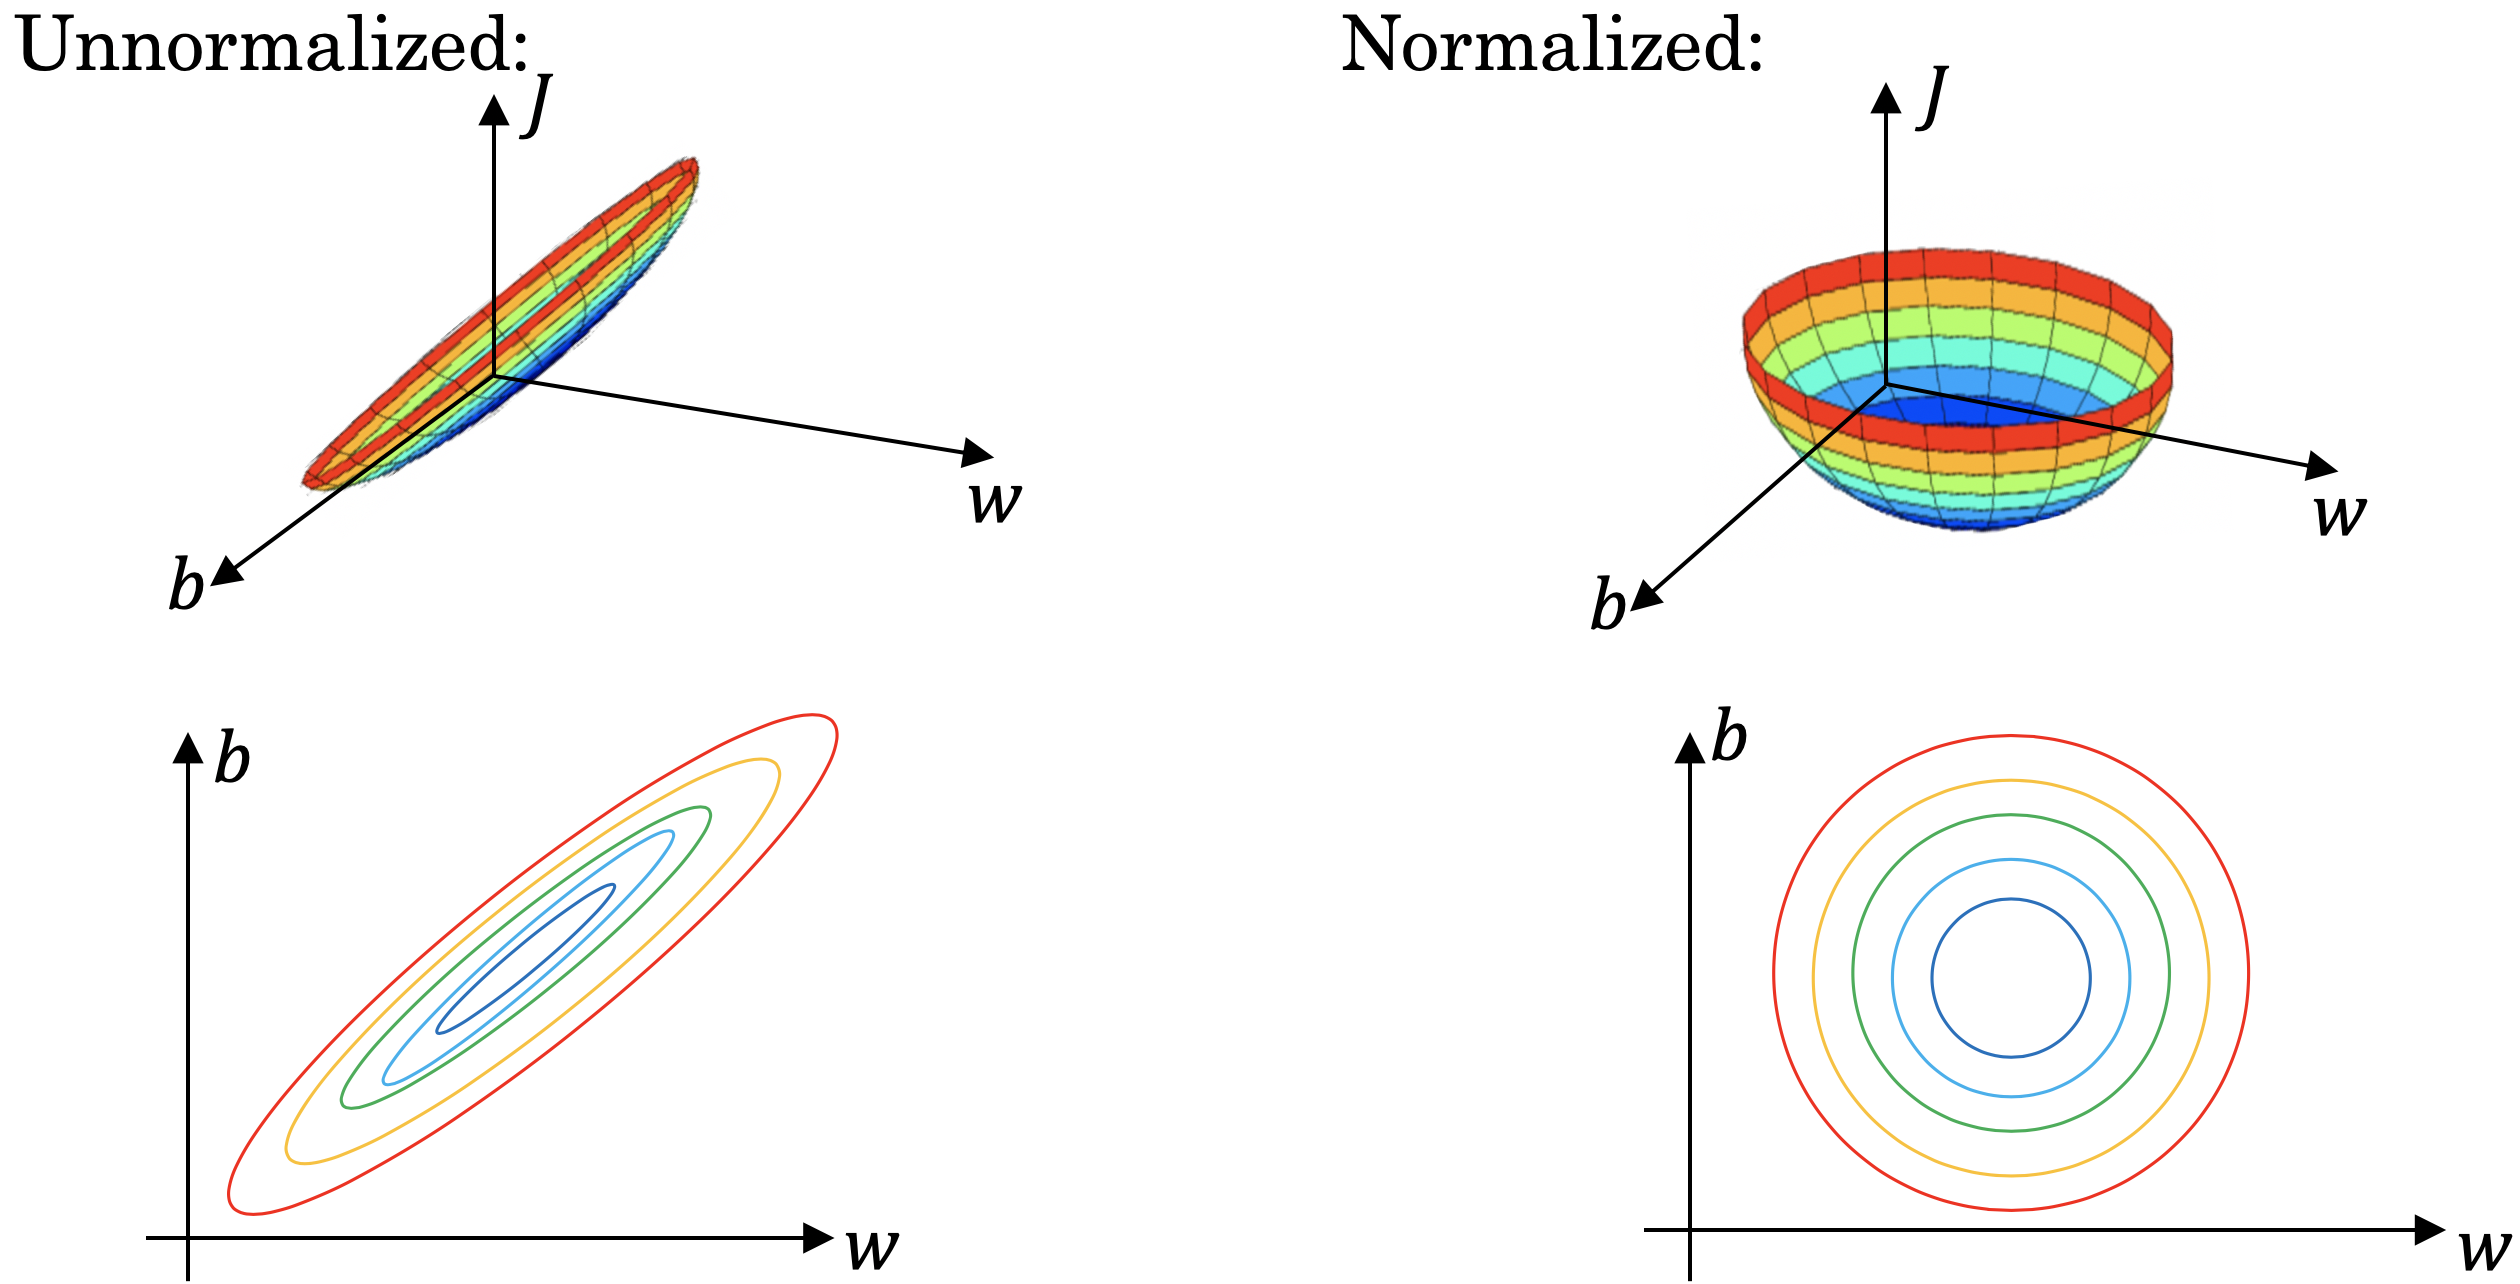
\includegraphics[width=.8\textwidth]{images/08featscale.png}
    \caption{Coutour of normalized and non-normalized cost functions. Original images from \cite{deeplearning_course}.}
    \label{fig:08featscale}
\end{figure}

To avoid this problem, the min-max normalization is applied to each variable and is given by:
\begin{equation}
    x^{norm} = \frac{x - x^{min}}{x^{max} - x^{min}}
    \label{eq:08normalization}
\end{equation}
where $x^{norm}$ is the normalized values.  Here, $x^{min}$ and $x^{max}$ are the minimum and maximum values of each variable, respectively.  By applying this normalization, all data are bounded between $x_i \in [0, 1]$, and the elongation issue of the cost function can be resolved.

\subsubsection{Exploratory Data Analysis}
Exploratory data analysis was then conducted to gain insights into the data set.  First, the distribution of the flow rate was explored and shown in Figure \ref{fig:08flowrate_dist}.  Here, it can be seen that the flow rate follows a bi-modal distribution meaning that there are two different operating strategies: a high demand strategy and a low demand strategy.

\begin{figure}[h]
    \centering
    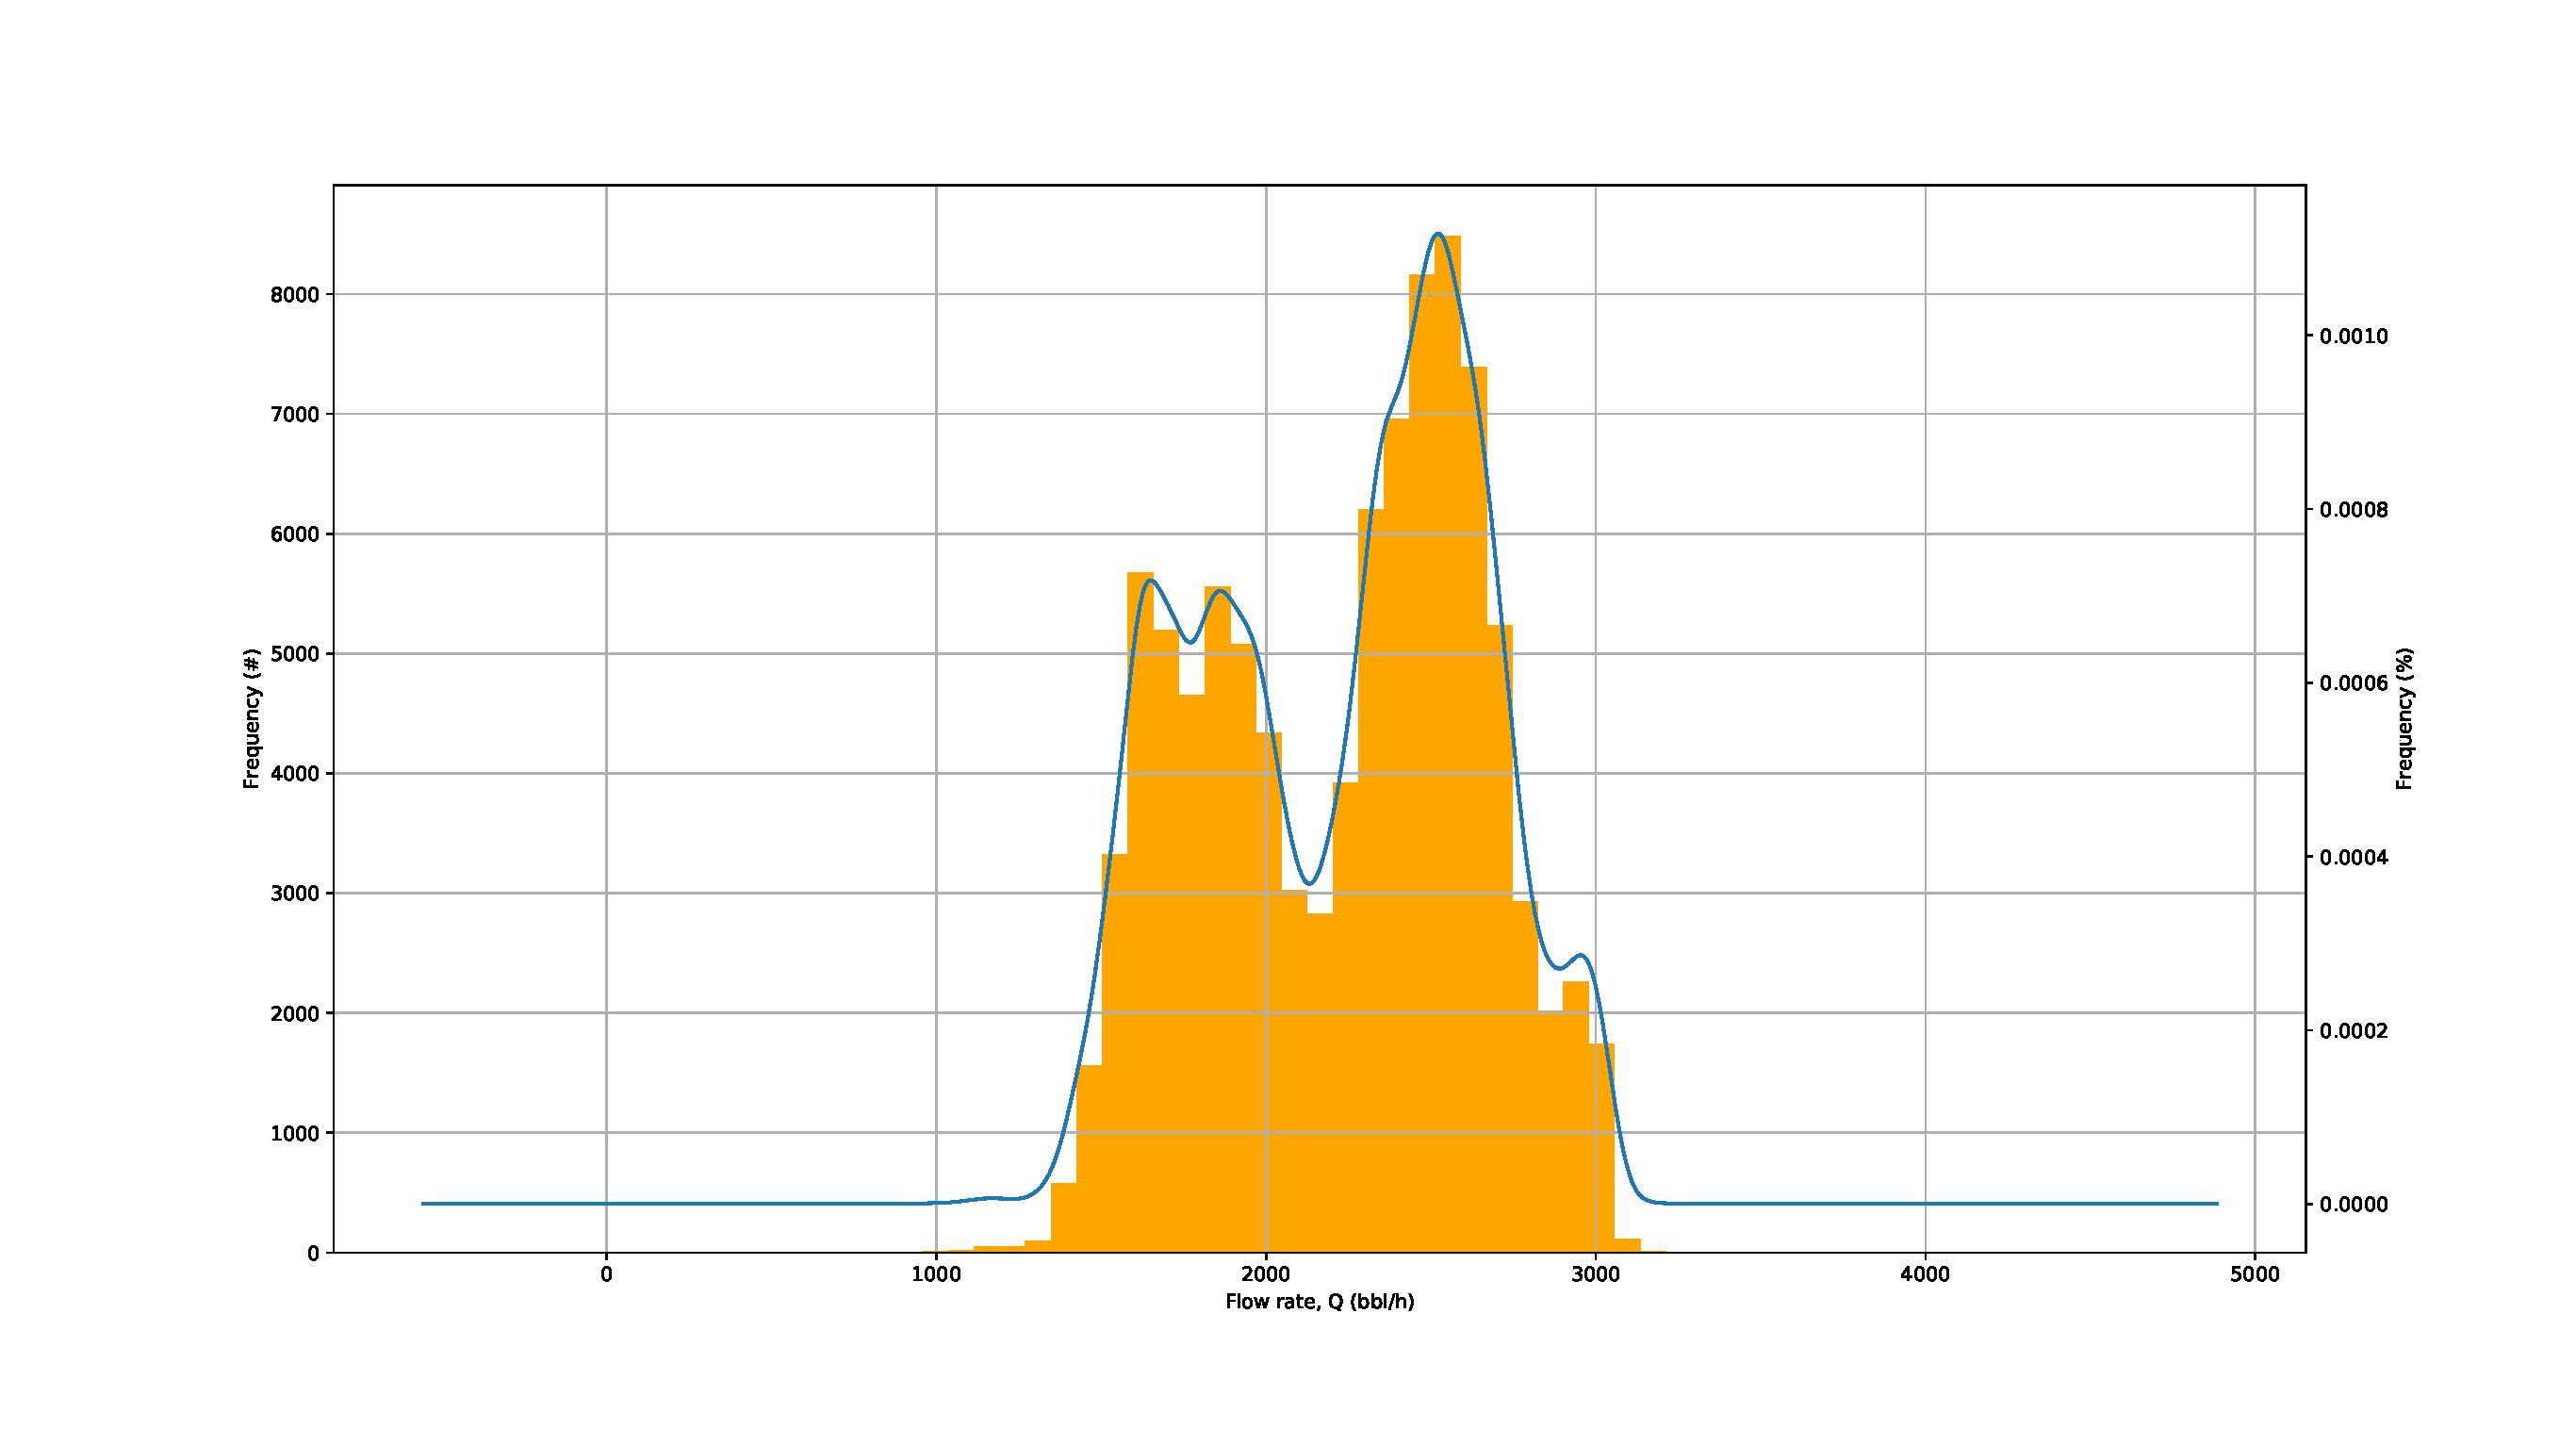
\includegraphics[scale=0.35]{images/08Flowrate_KDE.eps}
    \caption{Flow rate distribution of the pre-processed data set.}
    \label{fig:08flowrate_dist}
\end{figure}

To segregate the two Gaussian distributions, DBSCAN was used.  DBSCAN is a density-based algorithm for discovering clusters in large spatial data \cite{DBSCAN}. It contains two hyper parameters, $\epsilon$ and $min-points$.  The steps of DBSCAN is as follows:
\begin{enumerate}
    \item Normalize the data using Equation \ref{eq:08normalization} so each variable is weighted similarily.
    \item Create an $n-$dimensional sphere of radius $\epsilon$ around an initial data points.  Euclidean distance was used for the distance metric and is given by:
    \begin{equation}
        distance = \sqrt{(x_1^{(1)} - x_1^{(2)})^2 + (x_2^{(1)} - x_2^{(2)})^2 + ... + (x_m^{(1)} - x_m^{(2)})^2}
    \end{equation}
    where superscripts $1$ and $2$ are the first and second data points.
    \item If there are more than $min-points$ in this sphere, then all points within this sphere belong to the same cluster.
    \item Expand the cluster by recursively applying the above criteria to the edge points of the cluster.
    \item If the cluster can no longer be expanded, apply step 1 to a new data point currently not belonging to a cluster.
    \item If there are less than $min-points$ in this sphere, then the data point is ignored and we proceed to the next data point.
    \item Outlier data points are ones that fail to belong to any cluster.
\end{enumerate}
The resultant segregation created by DBSCAN is shown in Figure \ref{fig:08DBSCAN}. The hyper parameters for $\epsilon$ and $min-points$ are 1.13 and 10,000, respectively.  The first cluster (black) contained 56,738 data points while the second cluster (green) contained 36,779 data points.  The remaining 3953 data points (blue) were identified as outliers.
\begin{figure}[h]
    \centering
    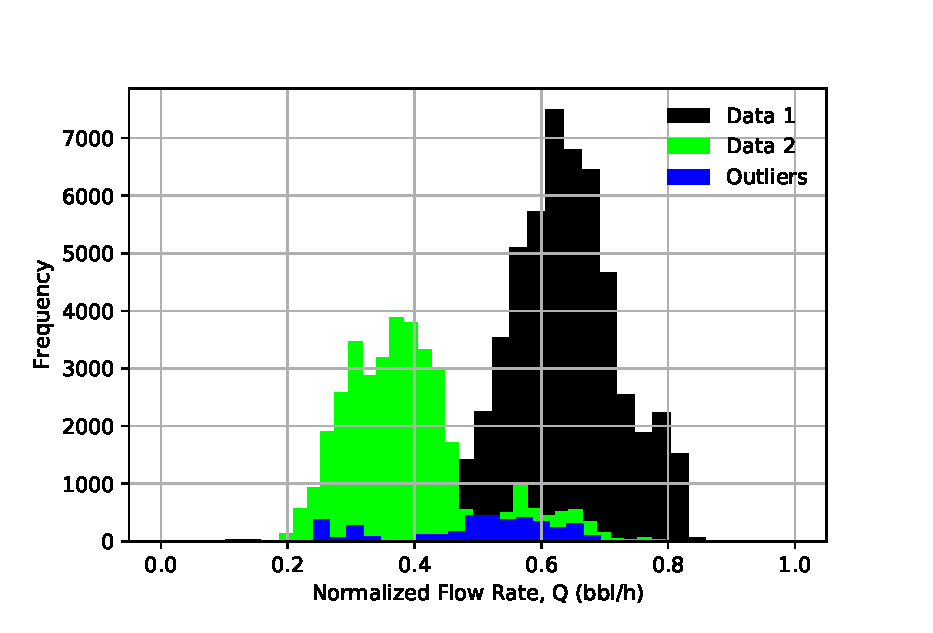
\includegraphics[scale=0.8]{images/08DBSCAN.eps}
    \caption{Clusters identified after applying the density-based scan.}
    \label{fig:08DBSCAN}
\end{figure}

The operating conditions of each cluster is shown in Figure \ref{fig:08cluster_variables}. The main differences are the flow rate, DRA usage, and pump usage.  Cluster 1 had 32\% higher average flow rate.  Cluster 1 also used substantially more DRA compared to cluster 1, where almost no DRA was used. Furthermore, the Cheyenne booster pump, Ault booster pump 1, Fort Lupton boooster pump, and Fort Lupton VFD were only used in cluster 1.  Ault booster pump 2 was only used in cluster 2.
\begin{figure}
    \centering
    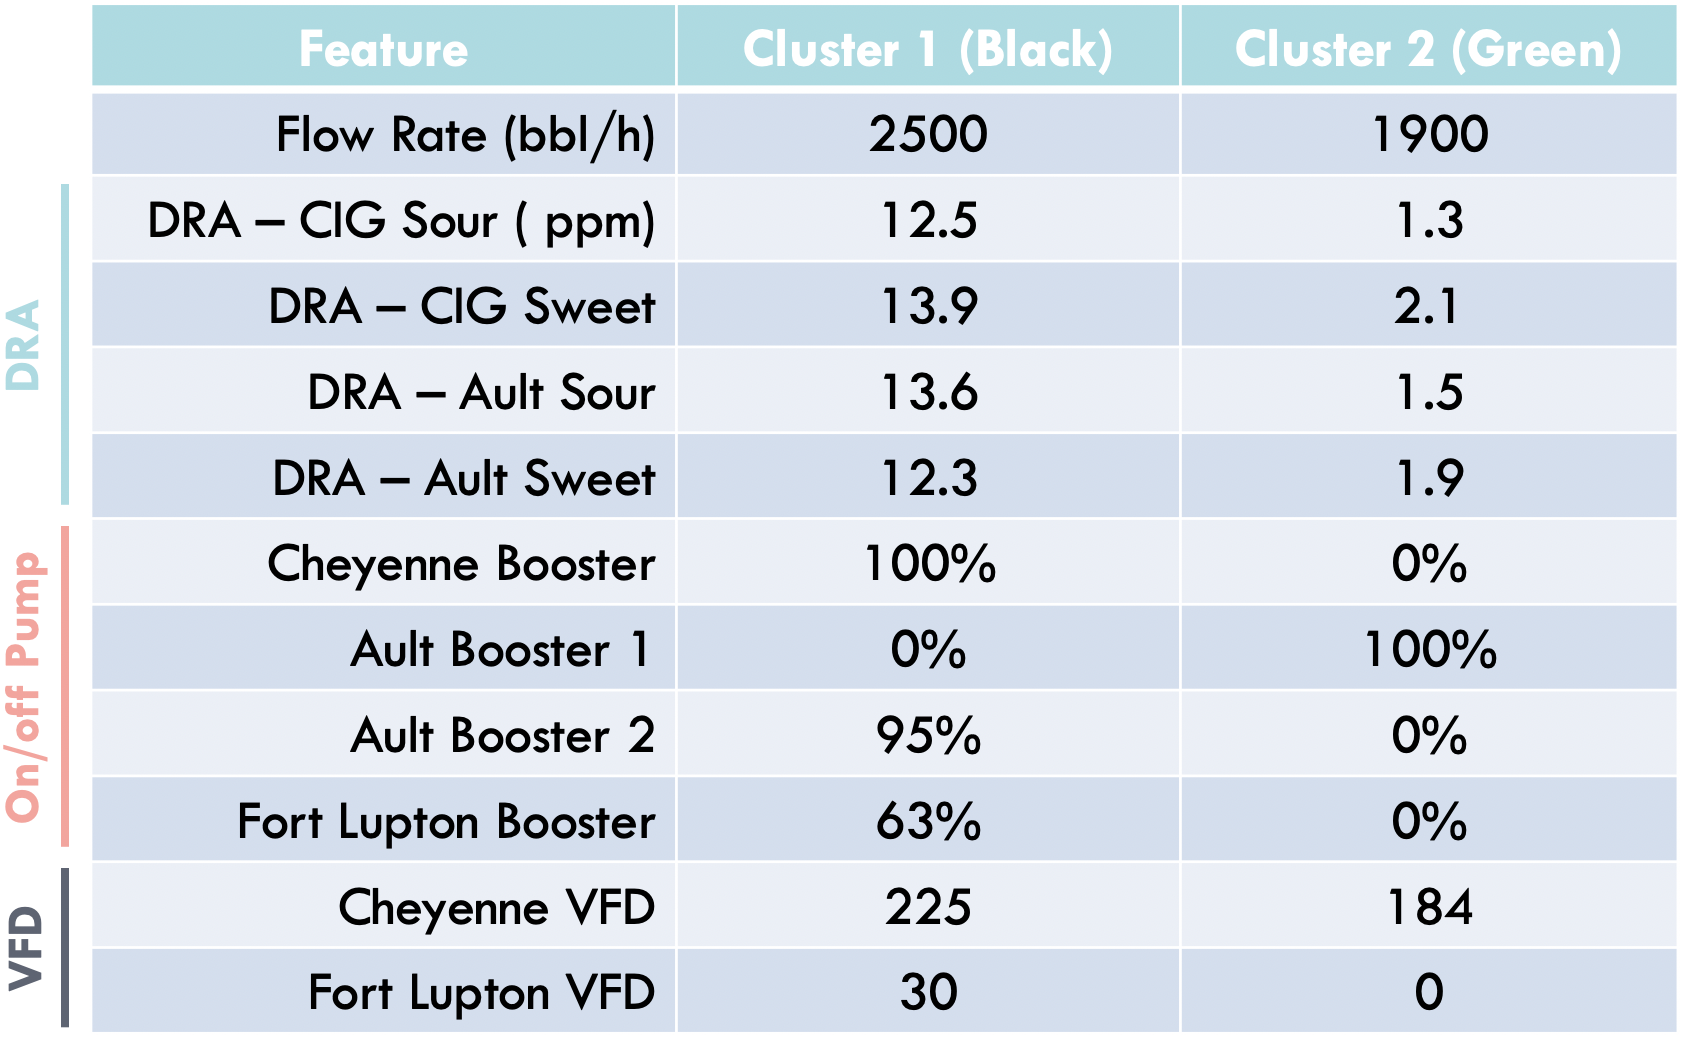
\includegraphics[width=0.8\textwidth]{images/08AvgChar.png}
    \caption{Average operating variables for the two operating conditions.}
    \label{fig:08cluster_variables}
\end{figure}

\subsubsection{Data Partitioning}
The data set was split into three sections to validate and test the machine learning models: training, validation, and testing.  The partition and description of each section is described in Table \ref{tab:08datapart}. The training data set is used to identify the machine learning model(s).  Then, the model is validated on un-trained data via the validation data set (sometimes called development data).  The error of the model on the validation data set, $e_{validation}$, should be similar to the training data error, $e_{train}$, to ensure that the model did not overfit to the training data. Finally, the model will be tested on the testing data to explore the performance of the model in live production.
\begin{table}[h]
    \centering
    {\setstretch{1.2}
    \begin{tabular}{ c | c | p{9cm}}
                            & \% of Data        &  Description \\
        \hline
        Training            &  90\%             
        &  Used to identify the machine learning model        \\
        
        Validation          &  5\%              
        &  Validates the performance of the machine learning model         \\
        
        Testing             &  5\%             
        &  Used to test performance of machine learning model on unseen data       \\             
    \end{tabular}}
    \caption{Features selected for machine learning models.}
    \label{tab:08datapart}
\end{table}

\subsubsection{Cost Function}

For all predictive models, the mean squared error (MSE) cost function is used and is given by:
\begin{equation}
    J(W) = \frac{1}{n}\sum\limits^n_{i=1}(\hat{y}_i - y_i)^2
    \label{eq:08MSE}
\end{equation}
where $n$ is the number of samples in the current optimization step.  $\hat{y}_i$ and $y_i$ are the $i^{th}$ predicted and actual labels, respectively. Here, $J$ is the loss. The MSE cost function was selected due to its convex nature \cite{deeplearning_course}.

To ensure adequate performance on the validation and testing data, the model must avoid overfitting to the training data.  One common way to reduce model complexity is by removing or reducing individual variables' impact on the model.  This study used a ridge regularization to reduce model complexity:
\begin{equation}
    J(W) = \frac{1}{n}\sum\limits^n_{i=1}(\hat{y}_i - y_i)^2 + \lambda \sum\limits^n_{j=1} W_j^2
    \label{eq:08MSE_wR}
\end{equation}
where $\lambda$ is the regularization penalty.  Here, as $\lambda \rightarrow \infty$, $W \rightarrow 0$.  That is, the larger $\lambda$ is, the stronger the weights are penalized. 

\subsubsection{Model Optimization}

The adaptive momentum (ADAM) gradient descent optimizer was used to update the weights and bias of the models.  The general gradient descent formulation is given by Equation \ref{eq:08GradientDescent} \cite{ADAM}.  
\begin{equation}
    \theta_j^{m+1} \leftarrow \theta_j^{m} - \alpha \frac{\partial J}{\partial \theta_j}
    \label{eq:08GradientDescent}
\end{equation}
where $\theta_j$ is the $j^{th}$ weight of the model.  $m$ represents the $m^{th}$ update of gradient descent and $\alpha$ is the learning rate.  ADAM improves upon Equation \ref{eq:08GradientDescent} by computing an adaptive learning rate for each parameter. To do so, the exponentially decaying average of the past gradients and squared gradients of the weights and biases are computed and stored using Equations \ref{eq:08momentW} to \ref{eq:08squared_momentb}.
\begin{equation}
    V_{dW} = \beta_1 V_{dW} + (1 - \beta_1)dW
    \label{eq:08momentW}
\end{equation}
\begin{equation}
    V_{db} = \beta_1 V_{db} + (1 - \beta_1)db
    \label{eq:08momentb}
\end{equation}
\begin{equation}
    S_{dW} = \beta_2 S_{dW} + (1 - \beta_2)dW^2
    \label{eq:08squared_momentW}
\end{equation}
\begin{equation}
    S_{db} = \beta_2 S_{db} + (1 - \beta_2)db^2
    \label{eq:08squared_momentb}
\end{equation}
where $V$ and $S$ are the estimates of the gradient and squared gradients, respectively.  $V$ and $S$ are typically initiated as zero vectors and are heavily biased towards zero at initial steps.  Hence, the biases for the initial terms are corrected using:
\begin{equation}
    V_{dW}^{corrected} = \frac{V_{dW}}{1 - \beta_1^t}
\end{equation}
\begin{equation}
    V_{db}^{corrected} = \frac{V_{db}}{1 - \beta_1^t}
\end{equation}
\begin{equation}
    S_{dW}^{corrected} = \frac{S_{dW}}{1 - \beta_2^t}
\end{equation}
\begin{equation}
    S_{db}^{corrected} = \frac{S_{db}}{1 - \beta_2^t}
\end{equation}
Combining the above equations, the weights and biases are updated using ADAM by:
\begin{equation}
    W_j \leftarrow W_j - \alpha \frac{V_{dW}^{corrected}}{S_{dW}^{corrected} + \epsilon}
\end{equation}
\begin{equation}
    b \leftarrow b - \alpha \frac{V_{db}^{corrected}}{S_{db}^{corrected} + \epsilon}
\end{equation}
where $\epsilon$ is a small scalar to avoid division by zero. The authors proposed values of 0.9, 0.999 and $10^{-8}$ for $\beta_1$, $\beta_2$, and $\epsilon$, respectively.

Due to the size of the data, batch gradient descent where all data are used to compute the gradient at each step is computationally infeasible.  Thus, mini-batch gradient descent was used where smaller batches of data were sampled from the original data set to perform parameter updates at each step.
\subsubsection{Performance Assessment}
The model performance were assessed using the following three ways:
\begin{enumerate}
    \item Root mean squared error (RMSE):
    \begin{equation}
        J = \sqrt{\frac{1}{n}\sum\limits^n_{i=1}(\hat{y}_i - y_i)^2}
        \label{eq:08RMSE}
    \end{equation}
    
    \item Mean absolute error (MAE):
    \begin{equation}
        J = \frac{1}{n}\sum\limits^n_{i=1}|\hat{y}_i - y_i|
        \label{eq:08MSE_Error}
    \end{equation}
    \item Coefficient of determination ($R^2$):
    \begin{equation}
        R^2 = 1 - \frac{\sum\limits^n_{i = 1}(\hat{y_i} - y_i)^2}{\sum\limits^n_{i = 1}(y_i - \bar{y_i})^2}
    \end{equation}
\end{enumerate}
Table \ref{tab:08performanceassessment} shows the advantages and disadvantages of each assessment metric.
\begin{table}[h]
    \centering
    {\setstretch{1.2}
    \begin{tabular}{ c | p{7cm} | p{7cm}}
         Method             & Advantages        &  Disadvantages \\
        \hline
        RMSE                &  Useful for identifying large errors                            &  Smaller errors are more muted        \\
        
        MAE                 &  Easy to interpret as all errors have the same weight           &  Inferior to RMSE when large errors are undesirable \\
        
        $R^2$               &  Easy to understand, $0 \leq R^2 \leq 1$                                         &  Valid only for linear relationships       \\             
    \end{tabular}}
    \caption{Constrained least squares validation and test plots.}
    \label{tab:08performanceassessment}
\end{table}

%%%%%%%%%%%%%%%%%%%%%%%%%%%%%%%%%%%%%%%%%%%%%%%%%%%%%%%%%%%%%%%%%%%%%
%
% Least squares model
%
%%%%%%%%%%%%%%%%%%%%%%%%%%%%%%%%%%%%%%%%%%%%%%%%%%%%%%%%%%%%%%%%%%%%%
\subsubsection{Linear Modelling}
\noindent
\textit{Least Squares} \\
The least squares regression was the first regression method to be explored, and was selected as the benchmark due to its simplicity and linear nature. The model structure of least squares is given as:
\begin{equation}
    \hat{y} = W^Tx + b
    \label{eq:08LS}
\end{equation}
where $x$ is a vector of features and the superscript $T$ represents the transpose operation.

Hyper parameters of the linear regression are shown in Table \ref{tab:08LSHparameters}.
\begin{table}[h]
    \centering
    {\setstretch{1.2}
    \begin{tabular}{ c | c}
        Hyper Parameter                  &  Value       \\
        \hline
        Epochs                           &  800      \\
        Minibatch size                   &  8192     \\
        Learning rate, $\alpha$          &  0.001    \\
        Regularization, $\lambda$          &  0.001  \\
    \end{tabular}}
    \caption{Hyper parameters for least squares regression.}
    \label{tab:08LSHparameters}
\end{table}
The performance assessment of the least squares model is shown in Table \ref{tab:08LSperformance}.
\begin{table}[h]
    \centering
    {\setstretch{1.2}
    \begin{tabular}{ c | c | c | c}
                             &  Training data    &  Validation data   &    Test data      \\
        \hline
        MAE                  &  98               &    98              &  102     \\
        RMSE                 &  127              &   127              &  135    \\ 
        $R^2$                &  0.91             &   0.91             &  0.70   \\
    \end{tabular}}
    \caption{Performance assessment for the least squares model.}
    \label{tab:08LSperformance}
\end{table}
The model performance on the validation and test data sets are shown in Figures \ref{fig:08LSValidation} and \ref{fig:08LSTest}.
\begin{figure}[h]
     \centering
     \begin{subfigure}[b]{0.48\textwidth}
         \centering
         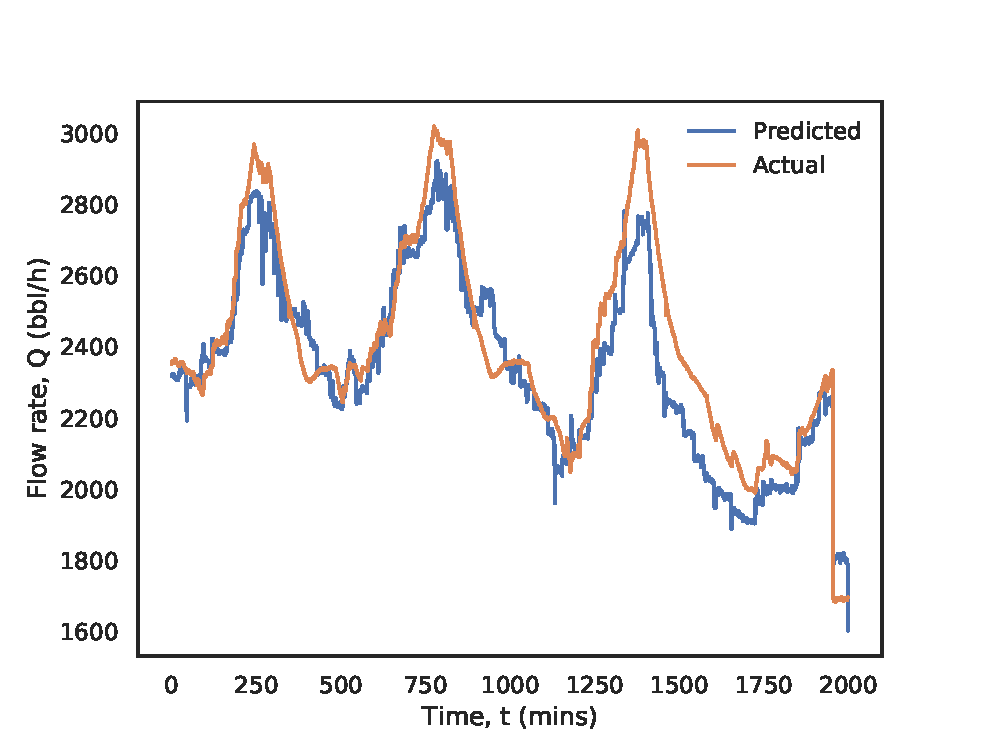
\includegraphics[width=\textwidth]{images/08ls_validation.eps}
         \caption{Predicted vs. actual flow rate for the validation data set.}
         \label{fig:08LSValidation}
     \end{subfigure}
     \hfill
     \begin{subfigure}[b]{0.48\textwidth}
         \centering
         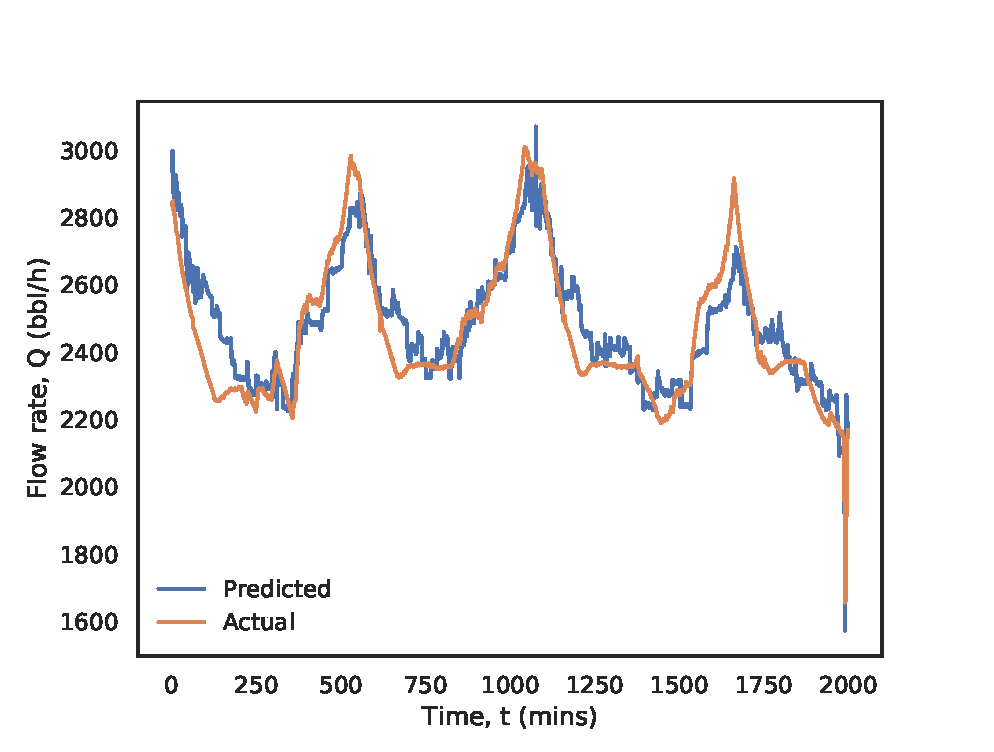
\includegraphics[width=\textwidth]{images/08ls_test.eps}
         \caption{Predicted vs. actual flow rate for the test data set.}
         \label{fig:08LSTest}
     \end{subfigure}
        \caption{Comparison of normal and abnormal density readings.}
        \label{fig:08LSPlots}
\end{figure}
The least squares model is given in Equation \ref{eq:08LS}.  Weights for $x_{11} - x_{14}$ were very small and were omitted.
\begin{multline}
    \hat{y} = 0.10x_1 + 0.15x_2 + 0.13x_3 + 0.04x_4 + 0.04x_5 + 0.09x_6 + 0.12x_7 - 0.01x_8 \\
    + 0.49x_9 + 0.02x_{10} + 0.09x_{11} - 0.18x_{15} + 0.30x_{16} - 0.05x_{17} + 0.04x_{18}
    \label{eq:08LS_eq}
\end{multline}
From Equation \ref{eq:08LS}, it can be seen that turning on the booster pump at Fort Lupton results in a decrease in flow rate.  Theoretically, this is impossible and is most likely caused by noise in the data.  To increase the models ability to reflect reality, engineering knowledge was injected into the model via constraining $x_1 - x_{10}$ to be strictly positive.

%%%%%%%%%%%%%%%%%%%%%%%%%%%%%%%%%%%%%%%%%%%%%%%%%%%%%%%%%%%%%%%%%%%%%
%
% Constrained LS
%
%%%%%%%%%%%%%%%%%%%%%%%%%%%%%%%%%%%%%%%%%%%%%%%%%%%%%%%%%%%%%%%%%%%%%

\noindent
\textit{Constrained Least Squares} \\
The new constrained least squares uses the same hyper parameters as shown in Table \ref{tab:08LSHparameters}.  Performance assessment of the constrained least squares is shown in Table \ref{tab:08ConstLSPerformance}.
\begin{table}[h]
    \centering
    {\setstretch{1.2}
    \begin{tabular}{ c | c | c | c}
                             &  Training data    &  Validation data   &    Test data      \\
        \hline
        MAE                  &  98               &    98              &  94     \\
        RMSE                 &  128              &   129              &  123    \\ 
        $R^2$                &  0.91             &   0.91             &  0.74   \\
    \end{tabular}}
    \caption{Performance assessment for the constrained least squares model.}
    \label{tab:08ConstLSPerformance}
\end{table}
The constrained least squares model performance on the validation and test data sets are shown in Figures \ref{fig:08CLSValidation} and \ref{fig:08CLSTest}. The results are nearly identical to the unconstrained model, with lower error in the test data set.
\begin{figure}[h]
     \centering
     \begin{subfigure}[b]{0.48\textwidth}
         \centering
         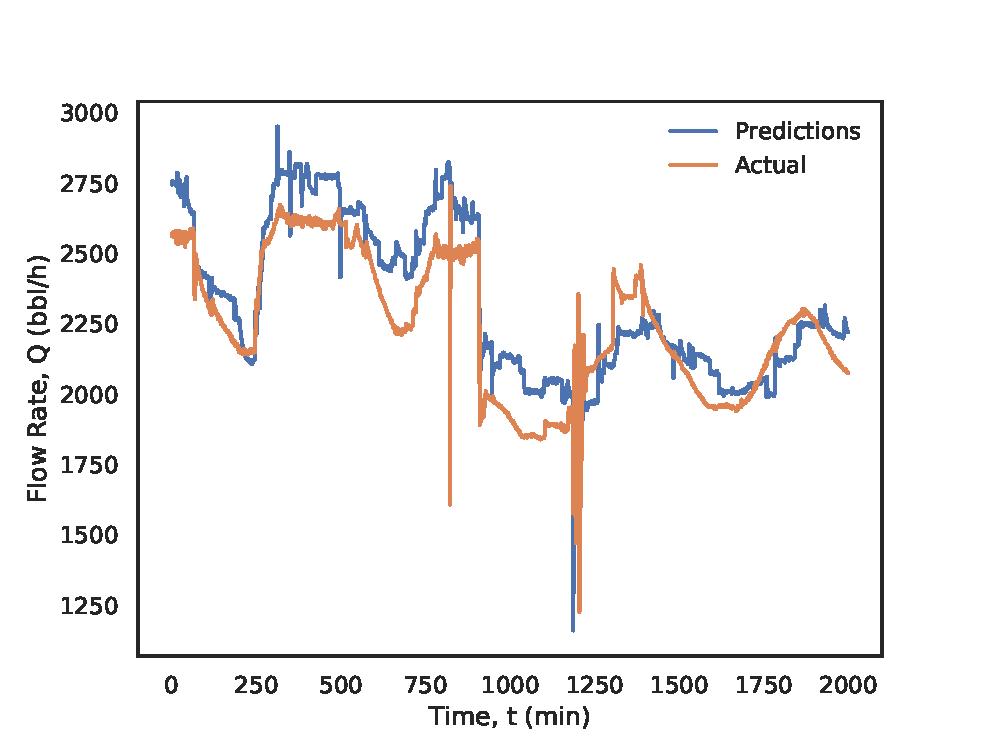
\includegraphics[width=\textwidth]{images/08ConstrainedLS_validation.eps}
         \caption{Predicted vs. actual flow rate for the validation data set.}
         \label{fig:08CLSValidation}
     \end{subfigure}
     \hfill
     \begin{subfigure}[b]{0.48\textwidth}
         \centering
         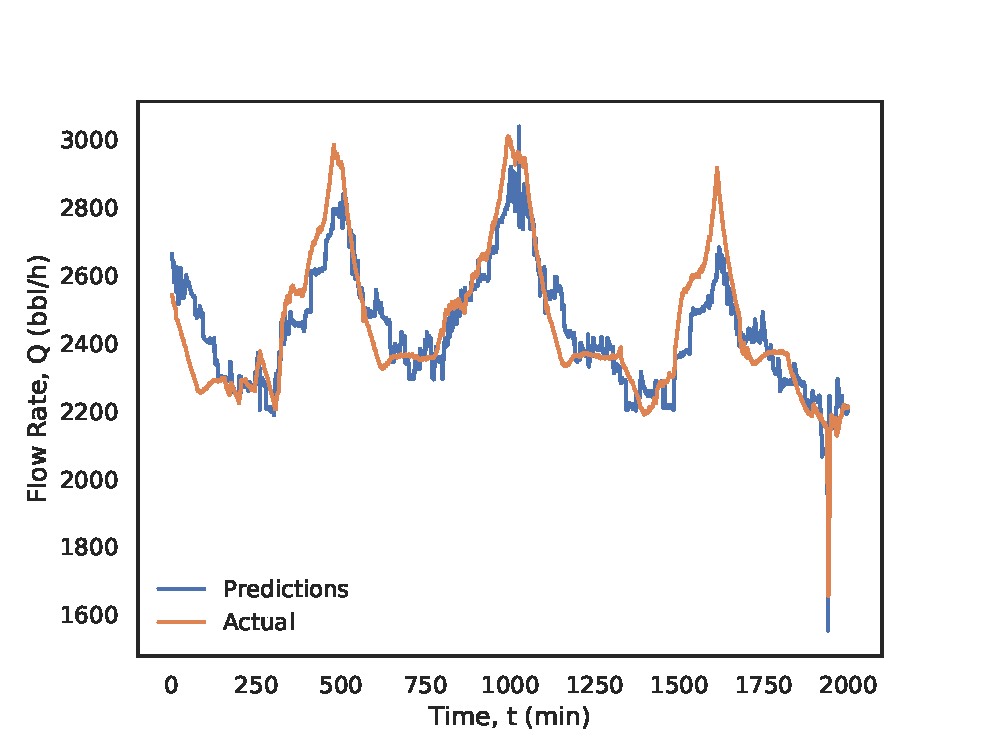
\includegraphics[width=\textwidth]{images/08ConstrainedLS_test.eps}
         \caption{Predicted vs. actual flow rate for the test data set.}
         \label{fig:08CLSTest}
     \end{subfigure}
        \caption{Constrained least squares validation and test plots.}
        \label{fig:08CLSPlots}
\end{figure}

The least squares model is given in Equation \ref{eq:08CLS}.  Weights for $x_{8}, x_{11} - x_{14}$ were very small and were omitted.
\begin{multline}
    \hat{y} = 0.10x_1 + 0.15x_2 + 0.13x_3 + 0.04x_4 + 0.04x_5 + 0.09x_6 + 0.11x_7 \\
    + 0.49x_9 + 0.02x_{10}  - 0.18x_{15} + 0.30x_{16} - 0.05x_{17} + 0.03x_{18}
    \label{eq:08CLS}
\end{multline}

\subsubsection{Non-linear Modelling}
To further increase the accuracy of the models, the following non-linear methods were explored for modelling the pipeline flow rate:
\begin{itemize}
    \item Polynomial models
    \begin{itemize}
        \item Quadratic model
        \item Square-root model
    \end{itemize}
    \item Feed-forward neural networks
    \begin{itemize}
        \item Small neural network (3 layers, 20 nodes per layer)
        \item Medium neural network (6 layers, 30 nodes per layer)
        \item Large neural network (8 layers, 40 nodes per layer)
    \end{itemize}
    \item Linear parameter-varying model
\end{itemize}

%%%%%%%%%%%%%%%%%%%%%%%%%%%%%%%%%%%%%%%%%%%%%%%%%%%%%%%%%%%%%%%%%%%%%
%
%  Quadratic and Sqrt models
%
%%%%%%%%%%%%%%%%%%%%%%%%%%%%%%%%%%%%%%%%%%%%%%%%%%%%%%%%%%%%%%%%%%%%%
\noindent
\textit{Polynomial Models} \\
The quadratic and square-root model structures are given by Equations \ref{eq:08quad_model} and \ref{eq:08sqrt_model}, respectively:
\begin{equation}
    \hat{y} = W_1^T X^2 + W^T_2 X + b
    \label{eq:08quad_model}
\end{equation}
\begin{equation}
    \hat{y} = W_1^T X^{1/2} + W^T_2 X + b
    \label{eq:08sqrt_model}
\end{equation}
where $W_1$ are the weights for the squared and square rooted variables for the quadratic and square-root models, respectively. Furthermore, $W_2$ are the weights for the original variables. The hyper parameters for both models are shown in Table \ref{tab:08poly_hp}.
\begin{table}[h]
    \centering
    {\setstretch{1.2}
    \begin{tabular}{ c | c}
        Hyper Parameter                  &  Value       \\
        \hline
        Epochs                           &  1000      \\
        Minibatch size                   &  8192     \\
        Learning rate, $\alpha$          &  0.001    \\
        Regularization, $\lambda$          &  0.001  \\
    \end{tabular}}
    \caption{Hyper parameters for least squares regression.}
    \label{tab:08poly_hp}
\end{table}

The performance assessment of the quadratic and square root models are shown in Table \ref{tab:08quad_performance} and \ref{tab:08sq_performance}, respectively. Compared to the constrained least squares, the MAE and RMSE went down by up to 10\% and 9\% when using the polynomial models, respectively.
\begin{table}[h]
    \centering
    {\setstretch{1.2}
    \begin{tabular}{ c | c | c | c}
                             &  Training data     &  Validation data    &    Test data      \\
        \hline
        MAE                  &  92      &    92     &  89    \\
        RMSE                 &  121     &   121     &  120   \\ 
        $R^2$                &  0.92    &   0.92    &  0.76  \\
    \end{tabular}}
    \caption{Performance assessment for the quadratic model.}
    \label{tab:08quad_performance}
\end{table}
\begin{table}[h]
    \centering
    {\setstretch{1.2}
    \begin{tabular}{ c | c | c | c}
                             &  Training data     &  Validation data    &    Test data      \\
        \hline
        MAE                  &  89      &  89     &  91   \\
        RMSE                 &   118    &  117    &  115  \\ 
        $R^2$                &    0.93  &   0.93  &  0.81 \\
    \end{tabular}}
    \caption{Performance assessment for the square root model.}
    \label{tab:08sq_performance}
\end{table}

The polynomial model performances are shown in Figures \ref{fig:08quad_validation} to \ref{fig:08sqrt_test}.  

\begin{figure}[h]
     \centering
     \begin{subfigure}[b]{0.45\textwidth}
         \centering
         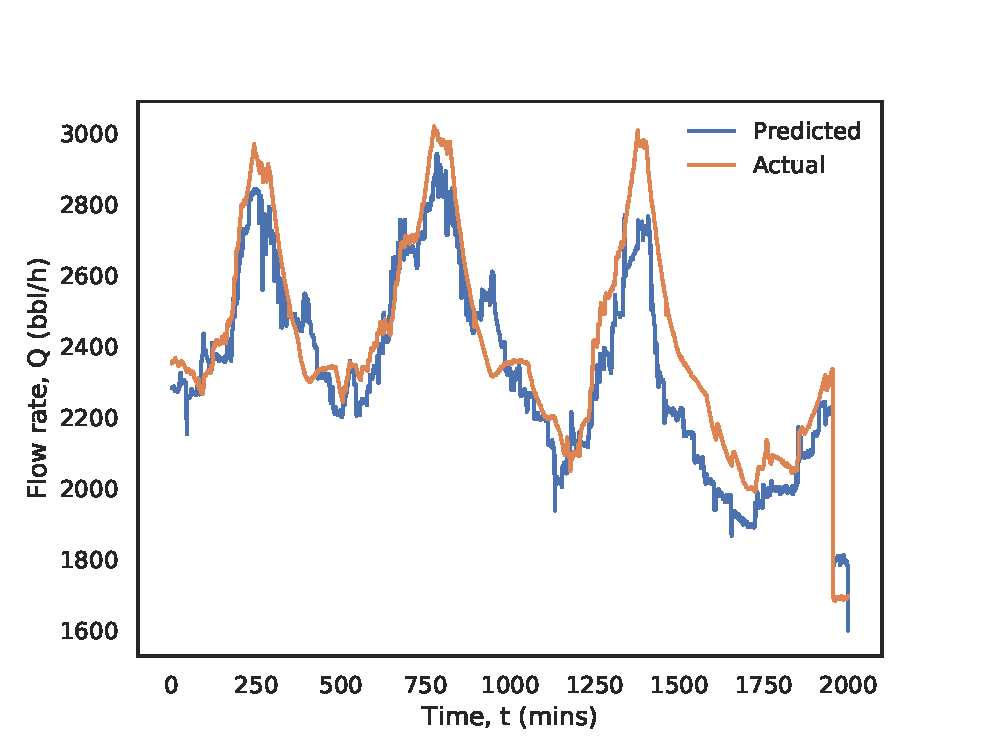
\includegraphics[width=\textwidth]{images/08quad_validation.eps}
         \caption{Predicted vs. actual flow rate for validation data using the quad. model.}
         \label{fig:08quad_validation}
     \end{subfigure}
     \begin{subfigure}[b]{0.45\textwidth}
         \centering
         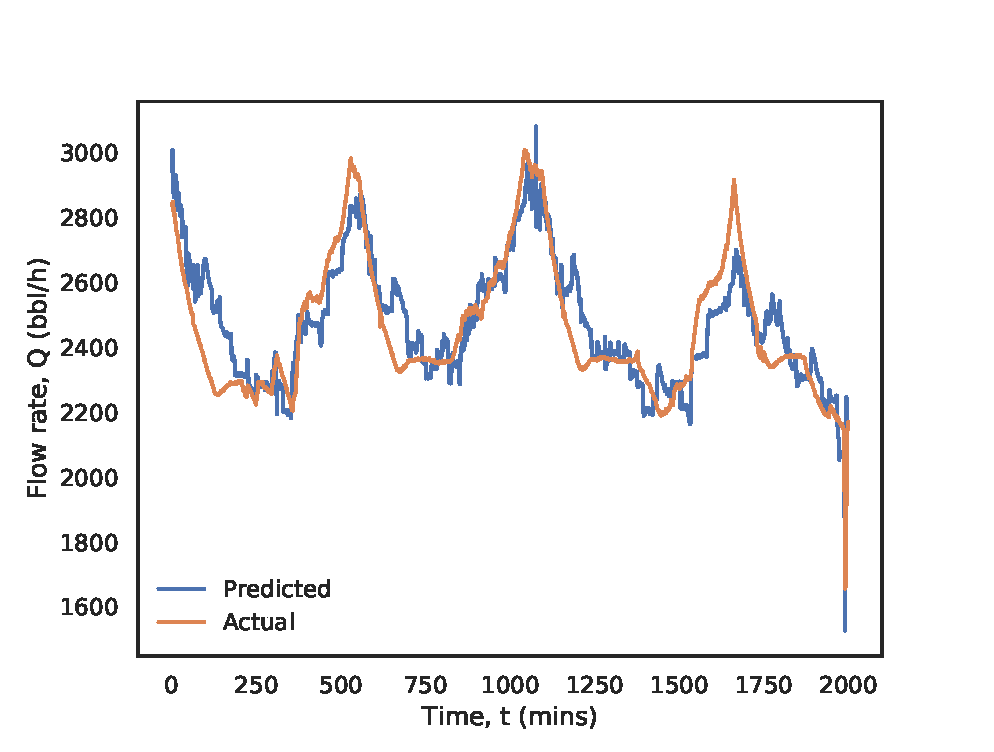
\includegraphics[width=\textwidth]{images/08quad_test.eps}
         \caption{Predicted vs. actual flow rate for the test data using the quadratic model.}
         \label{fig:08quad_test}
     \end{subfigure}
     \begin{subfigure}[b]{0.45\textwidth}
         \centering
         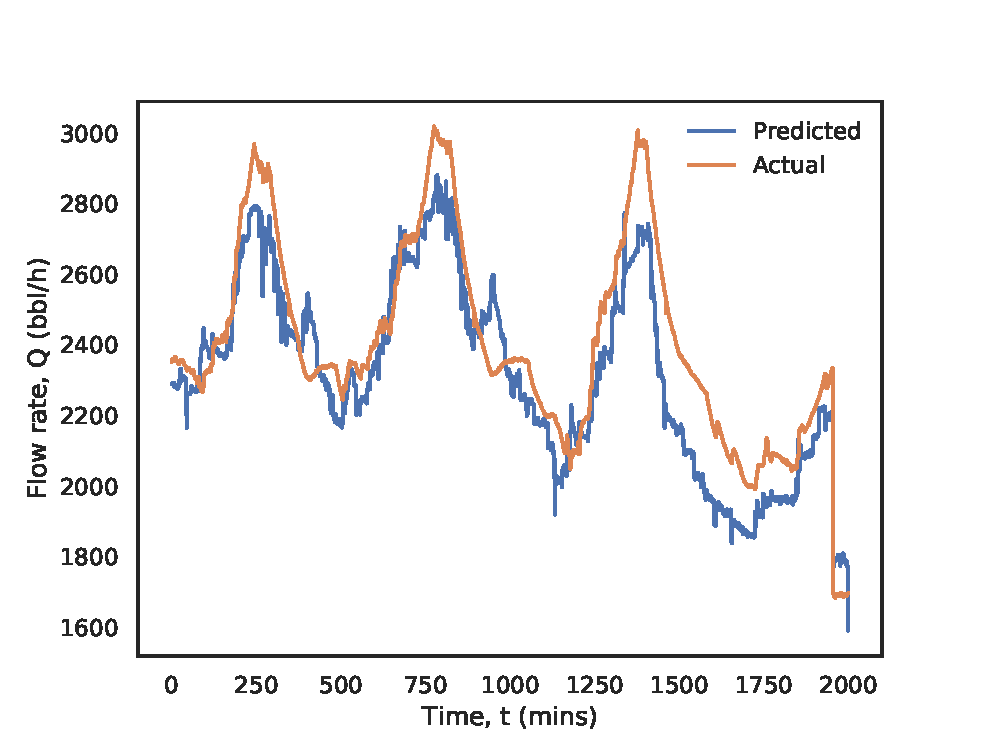
\includegraphics[width=\textwidth]{images/08sqrt_validation.eps}
         \caption{Predicted vs. actual flow rate for the validation data using the sqrt. model.}
         \label{fig:08sqrt_validation}
     \end{subfigure}
     \begin{subfigure}[b]{0.45\textwidth}
         \centering
         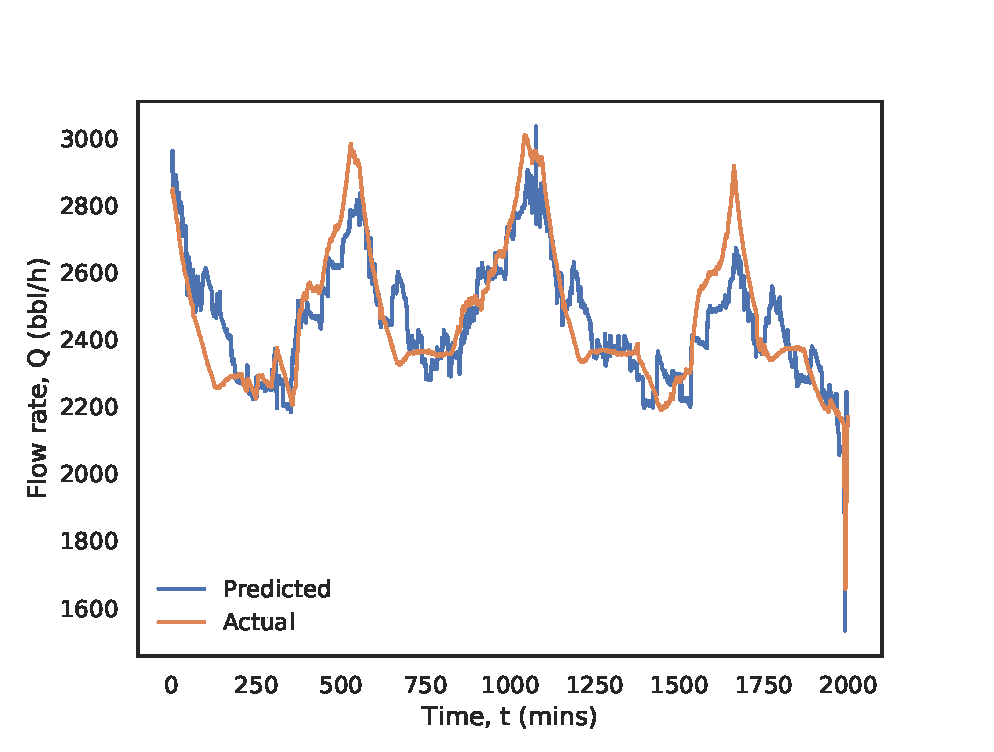
\includegraphics[width=\textwidth]{images/08sqrt_test.eps}
         \caption{Predicted vs. actual flow rate for the test data using the sqrt. model.}
         \label{fig:08sqrt_test}
     \end{subfigure}
        \caption{Polynomial regression validation and test plots.}
        \label{fig:08PolynomialPlots}
\end{figure}

%%%%%%%%%%%%%%%%%%%%%%%%%%%%%%%%%%%%%%%%%%%%%%%%%%%%%%%%%%%%%%%%%%%%%
%
% Neural Network Models
%
%%%%%%%%%%%%%%%%%%%%%%%%%%%%%%%%%%%%%%%%%%%%%%%%%%%%%%%%%%%%%%%%%%%%%
\noindent
\textit{Neural Network Models} \\
Neural networks are highly non-linear models that explore the individual and interaction effects of each variable with all other variables. The general structure of a neural network is shown in Figure \ref{fig:08NN}.  Neural networks are comprised of an input layer, some hidden layer(s), and an output layer.  The input layer consists of the input data, while the hidden layer(s) and output layer consists of fitted parameters, $W$ and $b$. In Figure \ref{fig:08NN}, $x_m$ denotes the $m^{th}$ input variable.  The superscript and subscript of $a$ denotes the hidden layer number and the node number in the corresponding layer, respectively.  Subscript $m_1$ to $m_r$ denotes the number of nodes in hidden layers 1 to $r$, respectively.  Finally, superscript $o$ denotes the output layer.
\begin{figure}[h]
    \centering
    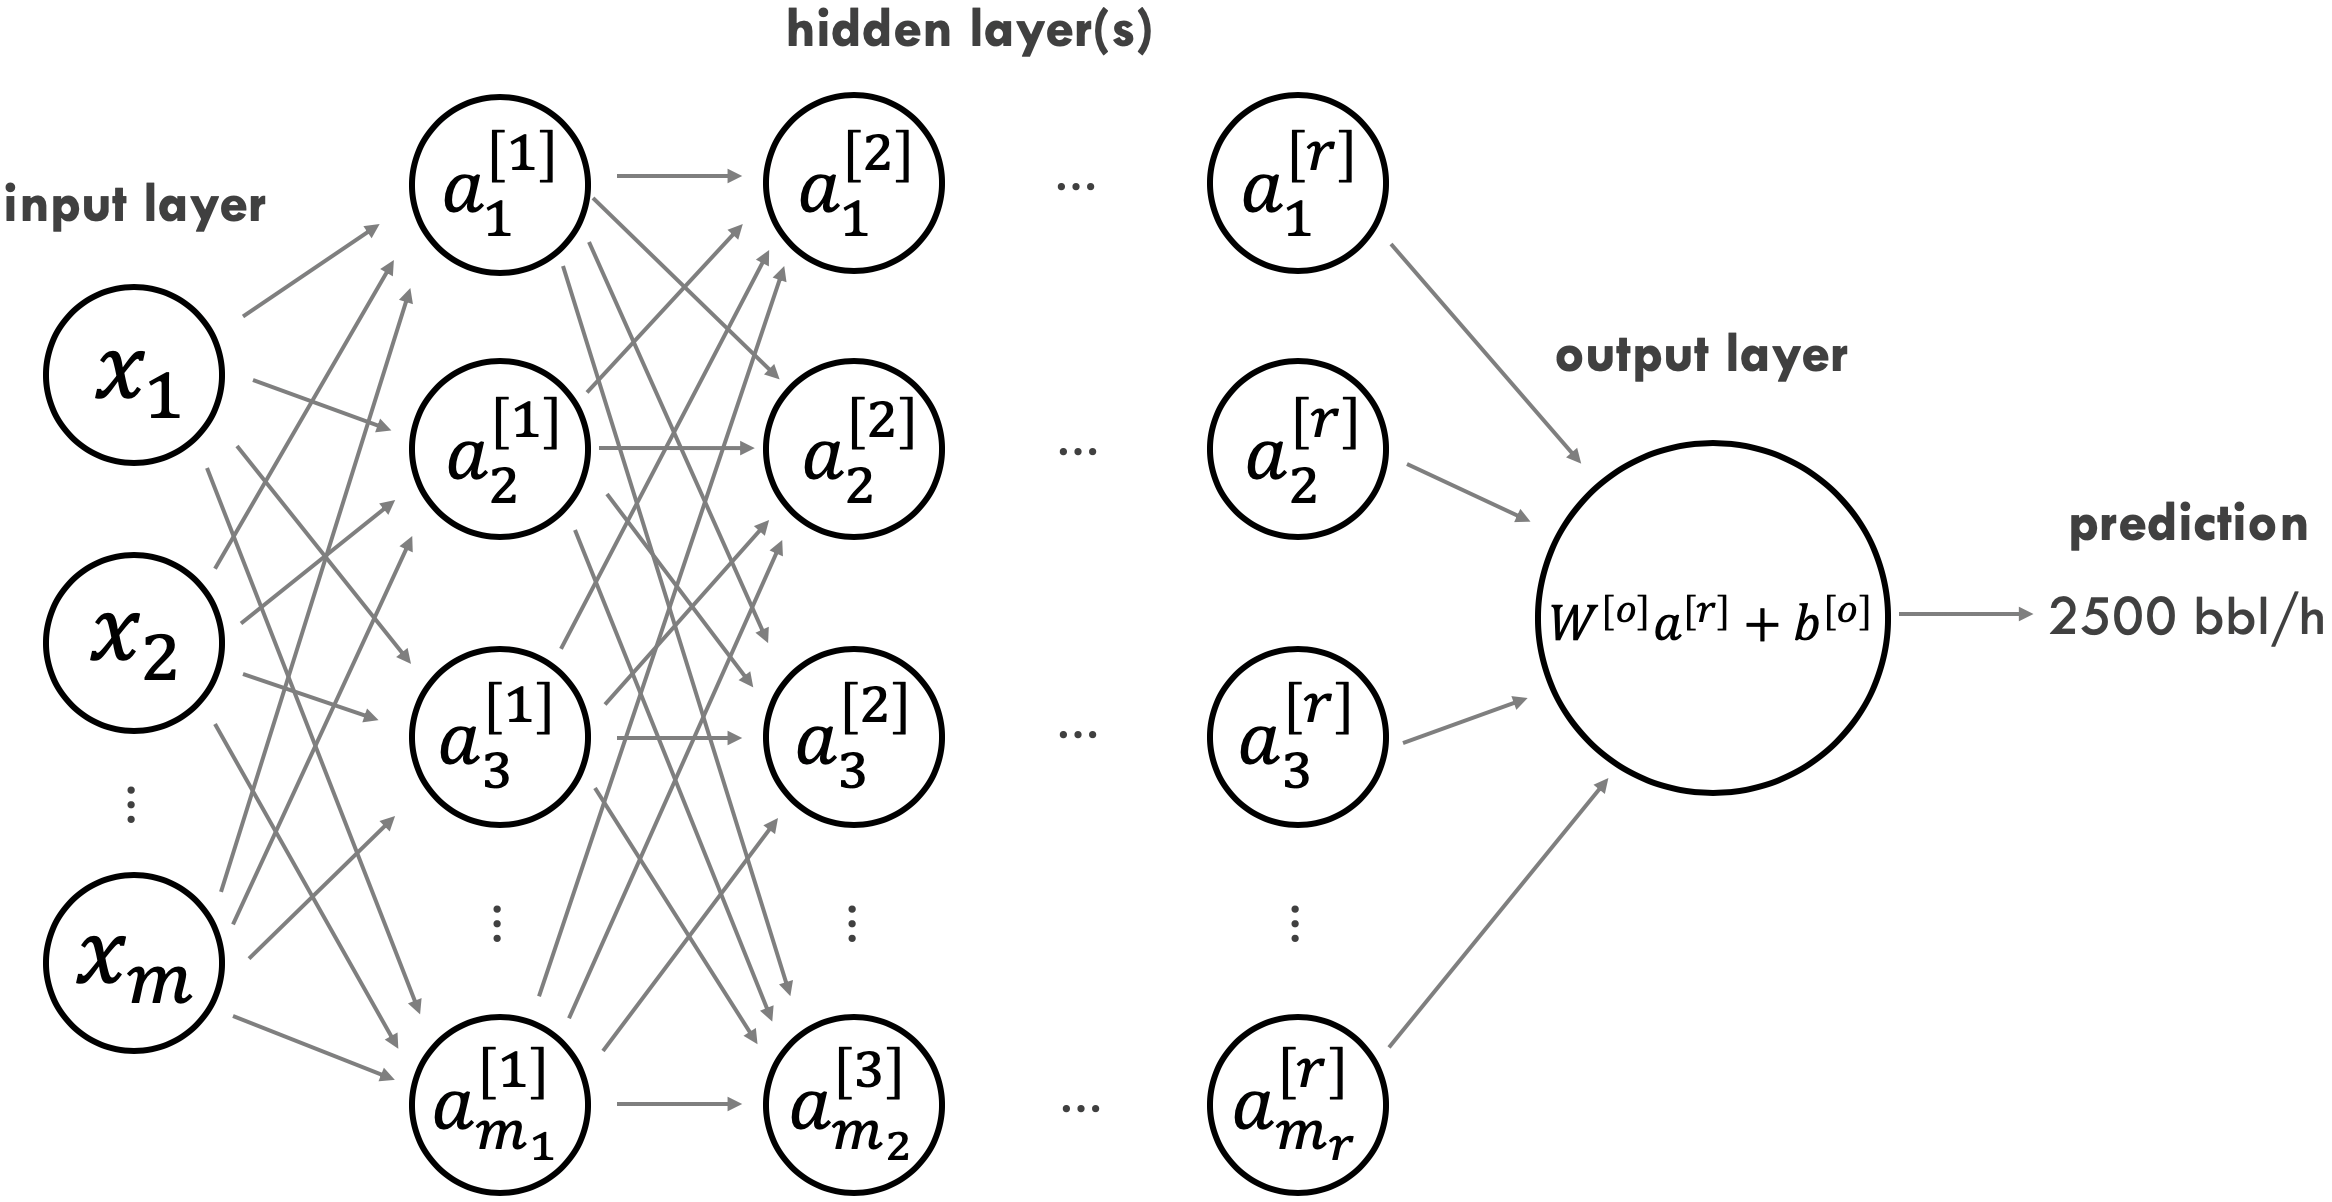
\includegraphics[width=0.9\textwidth]{images/08NN.png}
    \caption{Structure of a general neural network.}
    \label{fig:08NN}
\end{figure}

The details within a hidden layer's node is shown in Figure \ref{fig:08NNNode}.  First, the outputs from the previous layer's nodes are inputted into the node and is multiplied by the weights of the current node.  The current node's bias is then added.  Afterwards, the output is sent to a rectified linear unit (ReLU) activation function given by:
\begin{equation}
    a^{[i]}_j=\begin{cases}
        y, & \text{if $y\geq0$}.\\
        0, & \text{otherwise}.
    \end{cases}
    \label{eq:08ReLU}
\end{equation}
where $i$ and $j$ denotes any hidden layer and any node number, respectively.  
\begin{figure}[h]
    \centering
    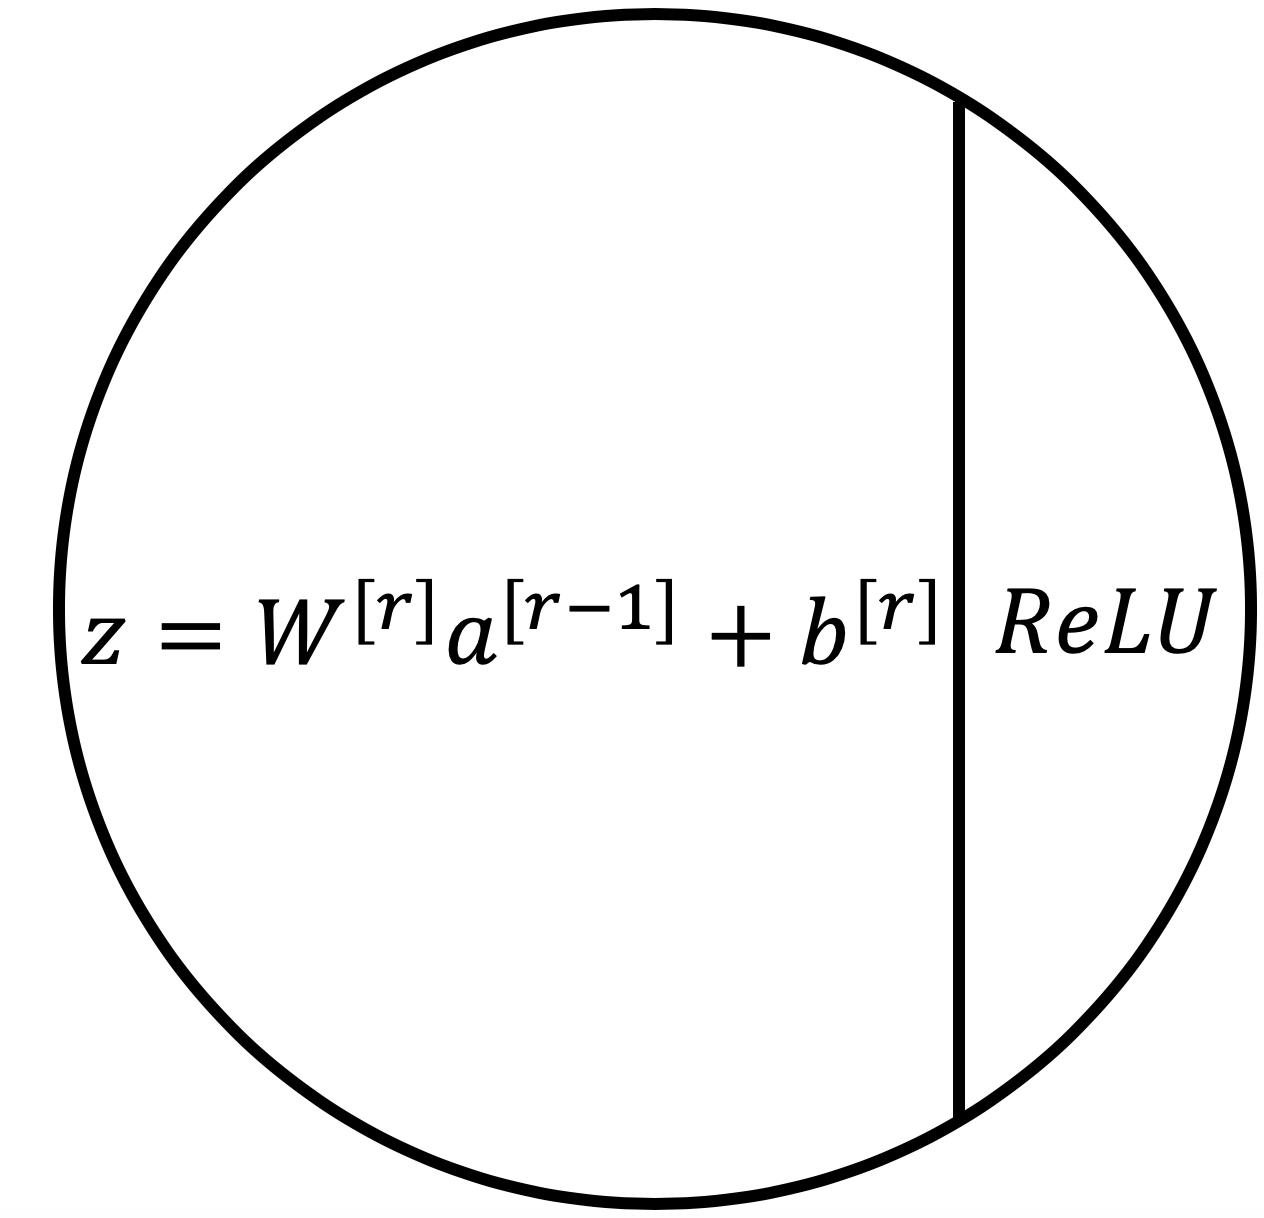
\includegraphics[width=0.3\textwidth]{images/08NNNode.png}
    \caption{Inside a hidden layer's node.}
    \label{fig:08NNNode}
\end{figure}

Mathematically, for one example $x$:
\begin{center}
    $z^{[1]}_j = W^{[1]}x + b^{[1]}$ \\
    $a^{[1]}_j = ReLU(z^{[1]}_j)$ \\
    $z^{[2]}_j = W^{[2]}a^{1}_j + b^{[2]}$ \\
    $a^{[2]}_j = ReLU(z^{[2]}_j)$ \\
    ... \\
    $z^{[r]}_j = W^{[r]}a^{r - 1}_j + b^{[r]}$ \\
    $a^{[r]}_j = ReLU(z^{[r]}_j)$ \\
    $y = W^{[o]}a^{[r]}_j + b^{[o]}$ \\  
\end{center}

The hyper parameters for each neural network is given in Table \ref{tab:08NN_hp}.
\begin{table}[h]
    \centering
    {\setstretch{1.2}
    \begin{tabular}{ c | c | c | c}
        Hyper Parameter                            &  Small NN  &  Med. NN  & Large NN       \\
        \hline
        Epochs                                     &  700       & 1000      & 1200  \\
        Minibatch size                             &  8192      & 8192      & 8192  \\
        Learning rate, $\alpha$                    &  0.001     & 0.001     & 0.001 \\
        Regularization, $\lambda$                  &  0.001     & 0.003     & 0.005 \\
        Number of layers                           &  3         & 6         & 8     \\
        Neurons per layer                          &  20        & 30        & 40    \\
        Activation function for hidden layers      & ReLU       & ReLU      & ReLU  \\
    \end{tabular}}
    \caption{Hyper parameters for the feed-forward neural network.}
    \label{tab:08NN_hp}
\end{table}

Tables \ref{tab:08small_nn} to \ref{tab:08large_nn} show the performance assessment of the small, medium and large neural networks.
\begin{table}[h]
    \centering
    {\setstretch{1.2}
    \begin{tabular}{ c | c | c | c}
                    &  Training data     &  Validation data    &    Test data      \\
        \hline
        MAE         &  48      &    50    &    87    \\
                    
        RMSE        &  66      &    69    &   117 \\ 
                    
        $R^2$       &  0.97    &   0.91   &   0.77  \\
    \end{tabular}}
    \caption{Performance assessment for the small neural network model.}
    \label{tab:08small_nn}
\end{table}

\begin{table}[h]
    \centering
    {\setstretch{1.2}
    \begin{tabular}{ c | c | c | c}
                    &  Training data     &  Validation data    &    Test data      \\
        \hline
        MAE         &  42     &     45   &   87    \\
                    
        RMSE        &  58     &     61   &   107   \\ 
                    
        $R^2$       &  0.98   &    0.90  &  0.83   \\
    \end{tabular}}
    \caption{Performance assessment for the medium neural network model.}
    \label{tab:08med_nn}
\end{table}

\begin{table}[h]
    \centering
    {\setstretch{1.2}
    \begin{tabular}{ c | c | c | c}
                    &  Training data     &  Validation data    &    Test data      \\
        \hline
        MAE         &  38     &    37   &    91   \\
                    
        RMSE        &  57     &    56   &   118 \\ 
                    
        $R^2$       &  0.99  &    0.94  &   0.77 \\
    \end{tabular}}
    \caption{Performance assessment for the large neural network model.}
    \label{tab:08large_nn}
\end{table}

The comparison of actual and predicted flow rates on the validation and test data for the neural nets are shown in Figures \ref{fig:08smallnn_valid} to \ref{fig:08largenn_test}.  
\begin{figure}[h]
     \centering
     \begin{subfigure}[b]{0.48\textwidth}
         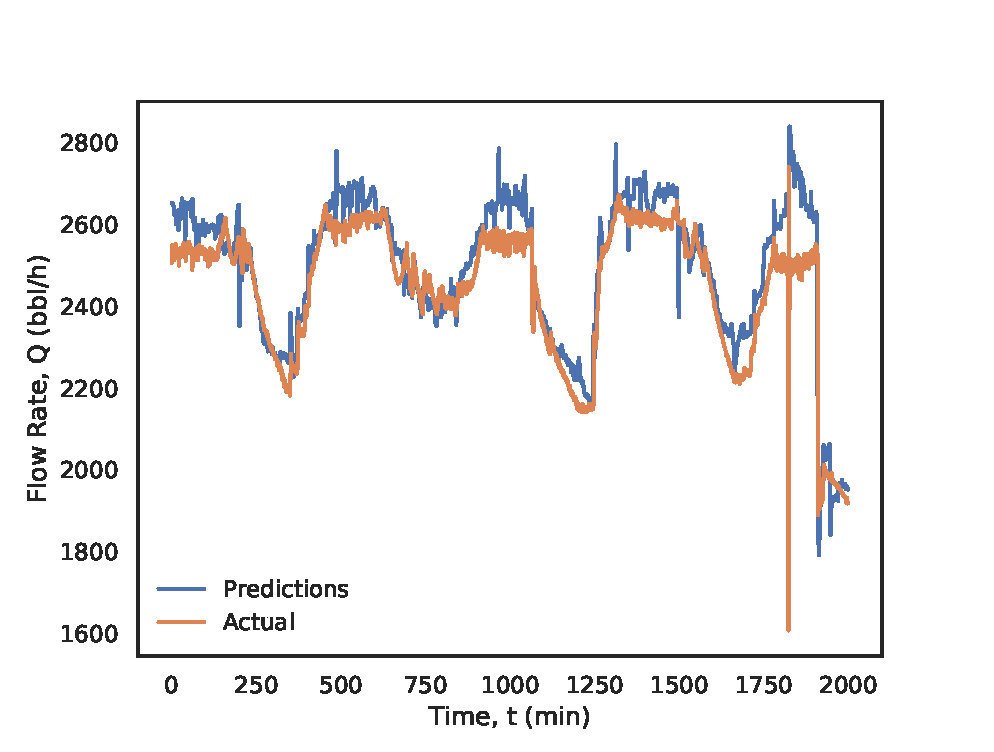
\includegraphics[width=\textwidth]{images/08smallnn_valid.eps}
         \caption{Predicted vs. actual flow rate for validation data using the small neural net.}
         \label{fig:08smallnn_valid}
     \end{subfigure}
     \begin{subfigure}[b]{0.48\textwidth}
         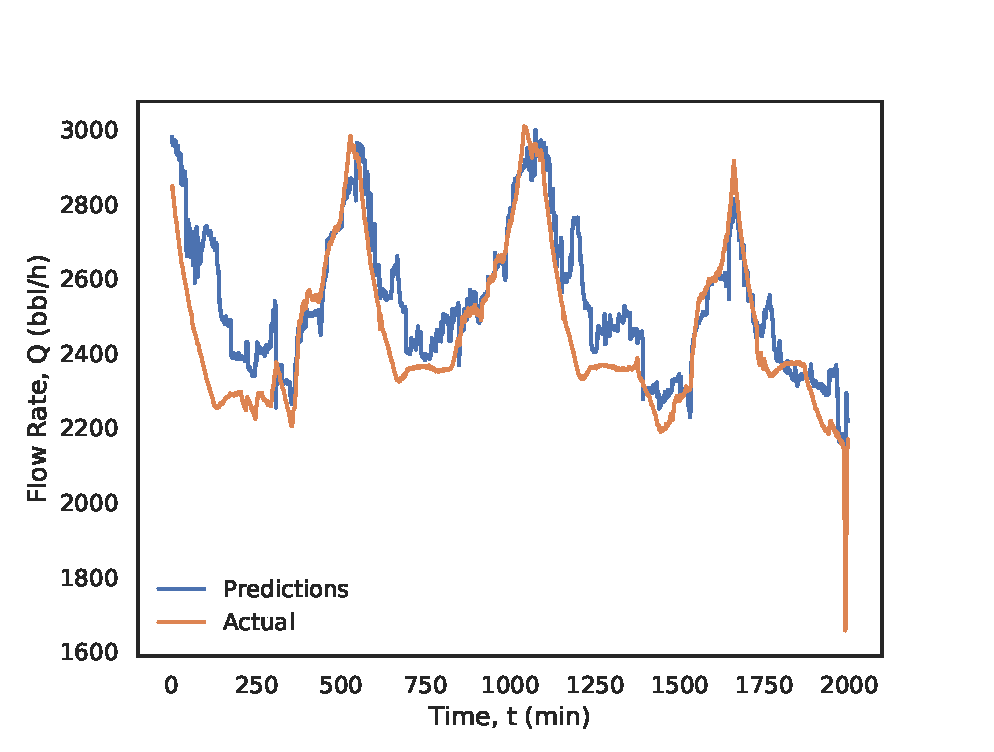
\includegraphics[width=\textwidth]{images/08smallnn_test.eps}
         \caption{Predicted vs. actual flow rate for the test data using the small neural net.}
         \label{fig:08smallnn_test}
     \end{subfigure}
     \begin{subfigure}[b]{0.48\textwidth}
         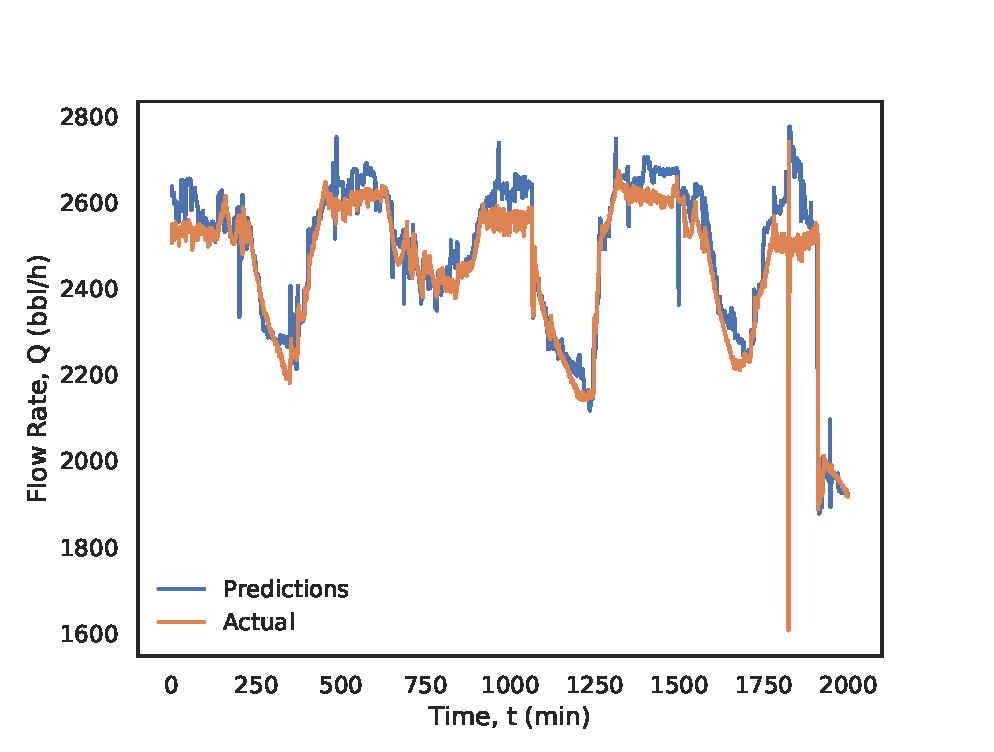
\includegraphics[width=\textwidth]{images/08mednn_valid.eps}
         \caption{Predicted vs. actual flow rate for the validation data using the med. neural net.}
         \label{fig:08mednn_valid}
     \end{subfigure}
     \begin{subfigure}[b]{0.48\textwidth}
         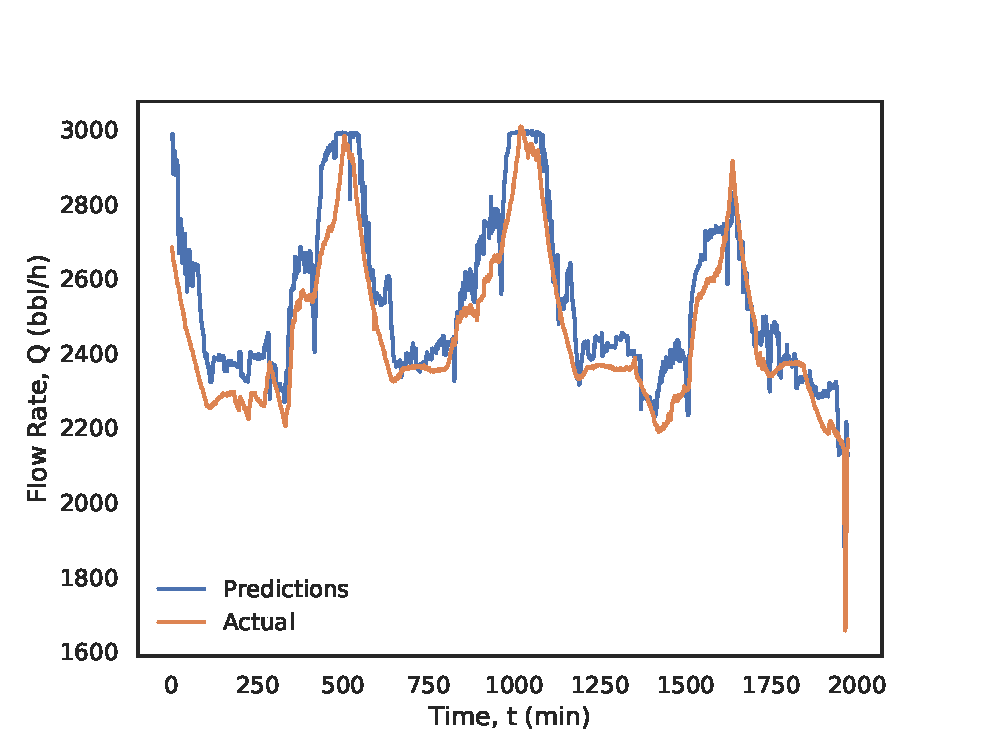
\includegraphics[width=\textwidth]{images/08mednn_test.eps}
         \caption{Predicted vs. actual flow rate for the test data using the med. neural net.}
         \label{fig:08mednn_test}
     \end{subfigure}
     \begin{subfigure}[b]{0.48\textwidth}
         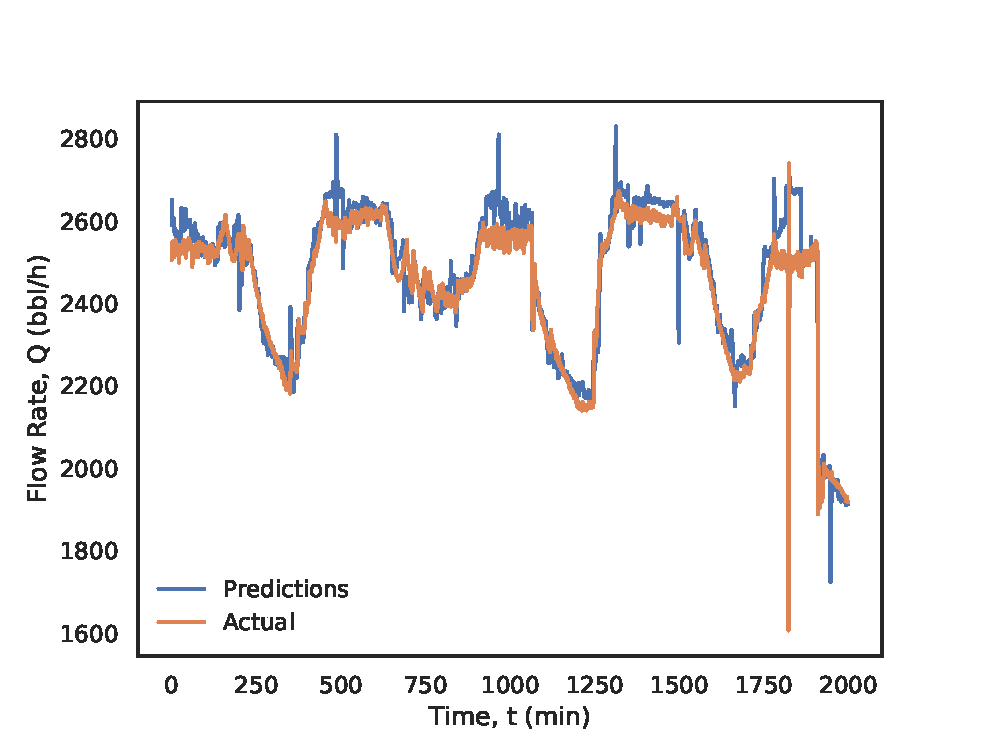
\includegraphics[width=\textwidth]{images/08largenn_valid.eps}
         \caption{Predicted vs. actual flow rate for the validation data using the large neural net.}
         \label{fig:08largenn_valid}
     \end{subfigure}
     \begin{subfigure}[b]{0.48\textwidth}
         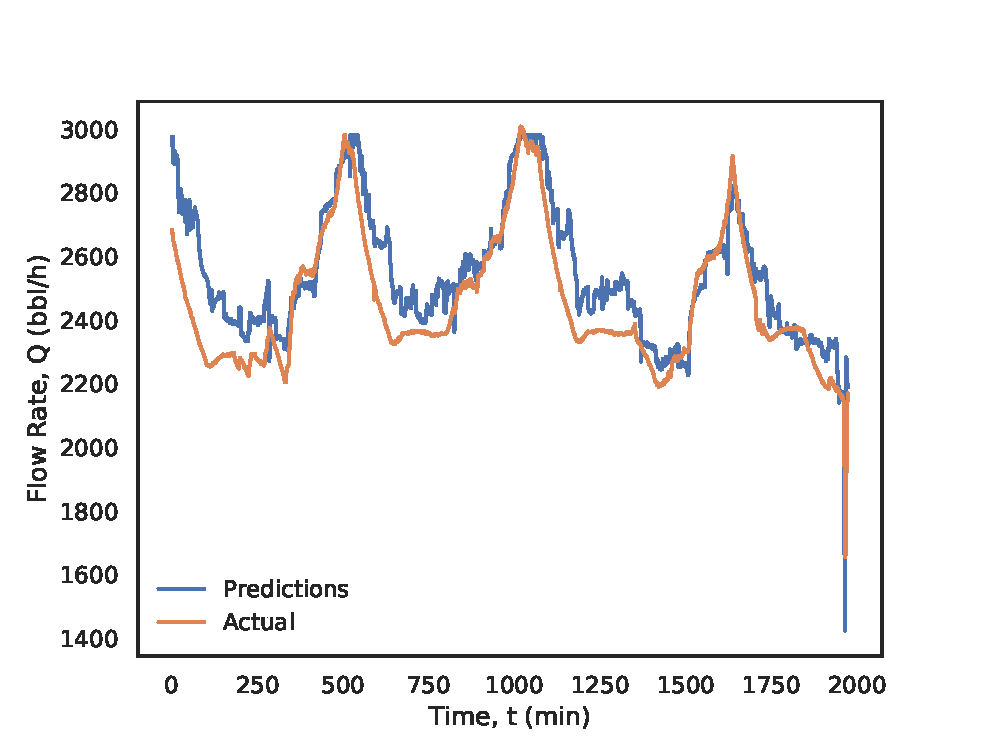
\includegraphics[width=\textwidth]{images/08largenn_test.eps}
         \caption{Predicted vs. actual flow rate for the test data using the large neural net.}
         \label{fig:08largenn_test}
     \end{subfigure}
        \caption{Feed-forward neural network validation and test plots.}
        \label{fig:08PolynomialPlots}
\end{figure}

%%%%%%%%%%%%%%%%%%%%%%%%%%%%%%%%%%%%%%%%%%%%%%%%%%%%%%%%%%%%%%%%%%%%%
%
% LPV MODELS
%
%%%%%%%%%%%%%%%%%%%%%%%%%%%%%%%%%%%%%%%%%%%%%%%%%%%%%%%%%%%%%%%%%%%%%
\noindent
\textit{Linear Parameter-varying Models} \\
Lastly, the linear parameter-varying model (LPV) is given by:
\begin{equation}
    \begin{split}
        \hat{y} = W_1^Tx + b_1 \\
        \hat{y} = W_2^Tx + b_2 \\
        ... \\
        \hat{y} = W_n^Tx + b_n \\
    \end{split}
    \label{eq:08LPV_structure}
\end{equation}
where $n \geq 1$ represents the number of linear models used to capture the data set. Here, $W_n$ and $b_n$ are the weights and biases corresponding to the $n^{th}$ model, respectively. For this study, two linear models were used to model the pipeline.  The models corresponded to the two clusters identified in Figure \ref{fig:08DBSCAN}.  Models 1 and 2 are identified from clusters 1 and 2, respectively.  During online implementation, the model will be selected based on the Euclidean distance between the features of the new data and the centroid of the two clusters.  However, if the distance exceeds 1.15 in both cases, the data will be labeled as anomalous.

The performance assessment of the two LPV models are shown in Tables \ref{tab:08cluster1_reg} and \ref{tab:08cluster2_reg}. 
\begin{table}[h]
    \centering
    {\setstretch{1.2}
    \begin{tabular}{ c | c | c | c}
                    &  Training data     &  Validation data    &    Test data      \\
        \hline
        MAE         &  90     &     90   &   96    \\
                    
        RMSE        &  115     &    116  &   120   \\ 
                    
        $R^2$       &  0.87   &    0.86  &   0.78   \\
    \end{tabular}}
    \caption{Performance assessment for cluster 1 regression model.}
    \label{tab:08cluster1_reg}
\end{table}

\begin{table}[h]
    \centering
    {\setstretch{1.2}
    \begin{tabular}{ c | c | c | c}
                    &  Training data     &  Validation data    &    Test data      \\
        \hline
        MAE         &  66     &    67   &   85   \\
                    
        RMSE        &  91     &    92   &   110 \\ 
                    
        $R^2$       &  0.90     &    0.89   &   0.57 \\
    \end{tabular}}
    \caption{Performance assessment for cluster 2 regression model.}
    \label{tab:08cluster2_reg}
\end{table}

The comparison of actual and predicted flow rates on the validation and test data for the LPV models are shown in Figures \ref{fig:08cluster1_valid} to \ref{fig:08cluster2_test}. 
\begin{figure}[h]
    \centering
     \begin{subfigure}[b]{0.48\textwidth}
         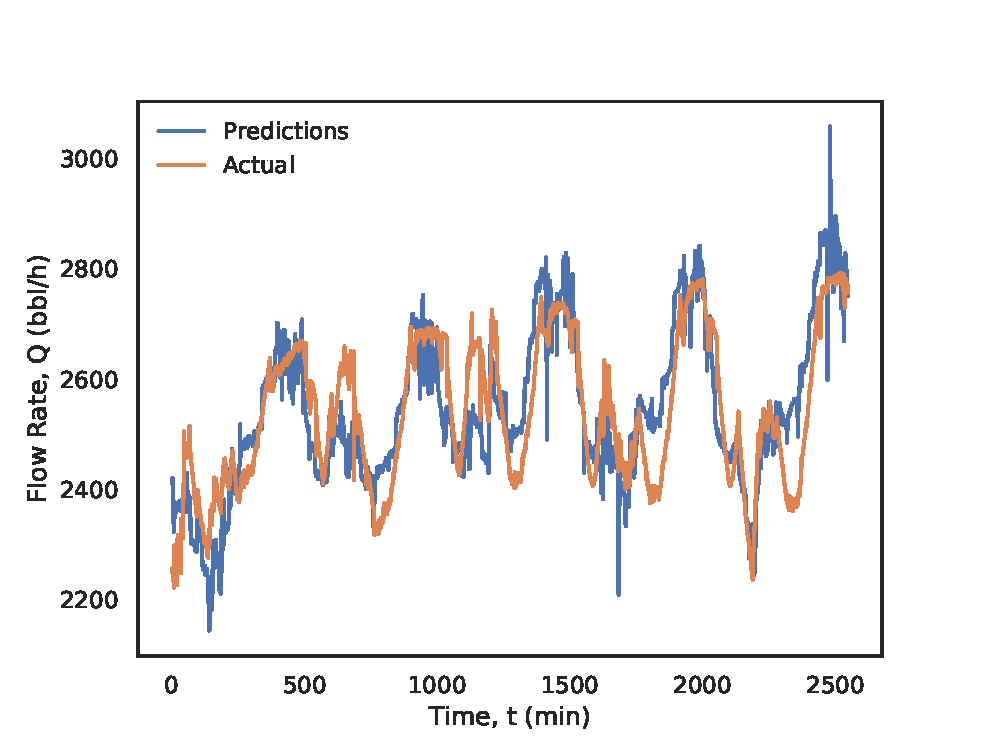
\includegraphics[width=\textwidth]{images/08cluster1_valid.eps}
         \caption{Predicted vs. actual flow rate for validation data using model 1.}
         \label{fig:08cluster1_valid}
     \end{subfigure}
     \begin{subfigure}[b]{0.48\textwidth}
         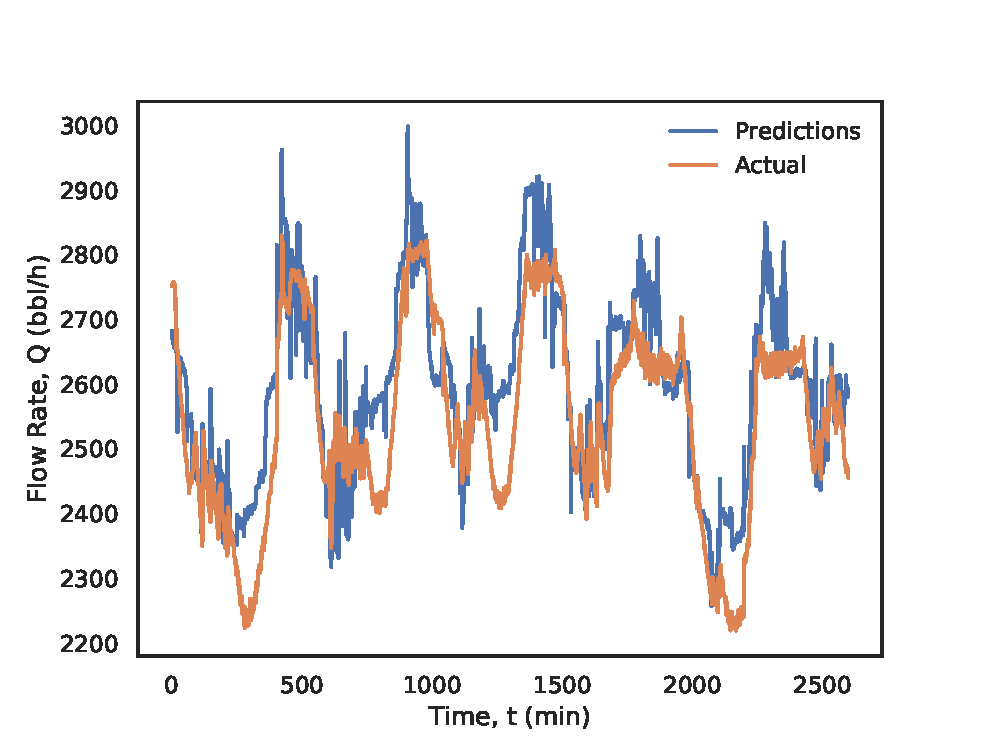
\includegraphics[width=\textwidth]{images/08cluster1_test.eps}
         \caption{Predicted vs. actual flow rate for the test data using model 1.}
         \label{fig:08cluster1_test}
     \end{subfigure}
     \begin{subfigure}[b]{0.48\textwidth}
         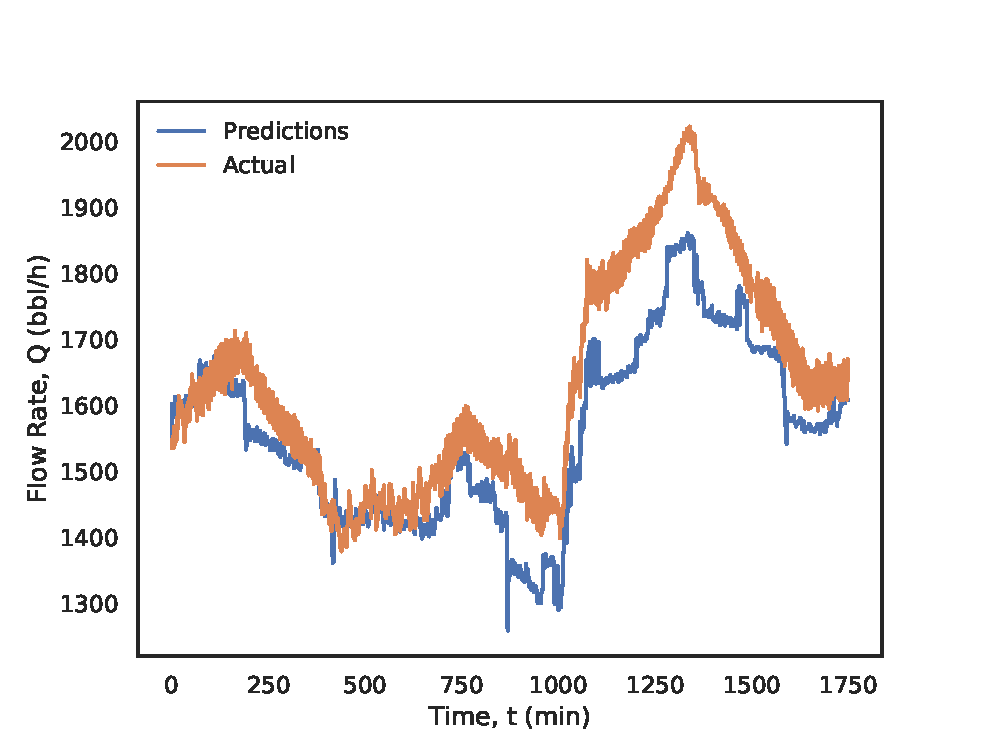
\includegraphics[width=\textwidth]{images/08cluster2_valid.eps}
         \caption{Predicted vs. actual flow rate for the validation data using model 2.}
         \label{fig:08cluster2_valid}
     \end{subfigure}
     \begin{subfigure}[b]{0.48\textwidth}
         \includegraphics[width=\textwidth]{images/08cluster2_test.eps}
         \caption{Predicted vs. actual flow rate for the test data using model 2.}
         \label{fig:08cluster2_test}
     \end{subfigure}
        \caption{Linear parameter-varying models' validation and test plots.}
        \label{fig:08PolynomialPlots}
\end{figure}

\subsubsection{Selected Model Structure}
Ultimately, a linear parameter-varying (LPV) model was selected to model this pipeline.  It is clear that the process is heavily non-linear due to the increase in accuracy when switching to a non-linear model structure; therefore, LPV models were selected due to their non-linear nature while still retaining the interpretability of linear models. To enhance credibility, any non-linear model can be approximated by a LPV model via the White's Theorem \cite{LPV}.

\subsubsection{Adaptive Machine Learning}
\paragraph{Online Learning vs. Incremental Learning}
\paragraph{ART: Adaptive Resonance Theory}
\paragraph{Implementation of Adaptive Machine Learning}

\begin{figure}
    \centering
    \includegraphics[width=\textwidth]{images/08IncrementalLearning.png}
    \caption{Importance Sampling Incremental Supervised learning architecture.}
    \label{fig:08ART}
\end{figure}

\subsection{Mixed Integer Linear Programming}
\subsection{Conceptual Software Design}
\subsection{Cost Savings and Impact on Society}


\chapter{RL Accelerated Economic MPC}
\input{chapters/Chapter09:RLandEMPC.tex}

\chapter{Automated Tuning using RL}
\input{chapters/Chapter10:RLTuning.tex}

\chapter{Concluding Remarks}
- RL is excellent in an highly mathematical complex problem that you have a simulator for like games.  But such processes don't exist in real life.
- MPC is the ideal outcome of RL everytime.
- RL has more exotic applications than control, and its value is most likely not in control.

\printbibliography

\end{document}